% !TeX spellcheck = pl_PL
\documentclass[a4paper,twoside]{article}
\usepackage{polski}
\usepackage[utf8]{inputenc}
\usepackage{graphicx}
\usepackage{amsmath}

%\usepackage[unicode, bookmarks=true]{hyperref} %do zakładek
\usepackage{tabto} % do tabulacji
\NumTabs{6} % globalne ustawienie wielkosci tabulacji
\usepackage{array}
\usepackage{multirow}
\usepackage{array}
\usepackage{dcolumn}
\usepackage{bigstrut}
\usepackage{color}
\usepackage[usenames,dvipsnames]{xcolor}
\usepackage{pdfpages}
\usepackage{sidecap}
\usepackage{wrapfig}
\usepackage{float}	%for figure& table placement in text

\setlength{\textheight}{24cm}
\setlength{\textwidth}{15.92cm}
\setlength{\footskip}{10mm}
\setlength{\oddsidemargin}{0mm}
\setlength{\evensidemargin}{0mm}
\setlength{\topmargin}{0mm}
\setlength{\headsep}{5mm}

\newcolumntype{M}[1]{>{\centering\arraybackslash}m{#1}}
\newcolumntype{N}{@{}m{0pt}@{}}

\graphicspath{ {./images/} }

\definecolor{nie}{RGB}{178,34,34}
\definecolor{tak}{RGB}{0,120,0}

% === Reset inkrementacji sekcji przy nowym parcie === %
\usepackage{titlesec}

\makeatletter
\@addtoreset{section}{part}
\makeatother
\titleformat{\part}[display]
{\normalfont\LARGE\bfseries\centering}{}{0pt}{}


\begin{document}
\bibliographystyle{plain}



\begin{titlepage}
\title{\huge Interfejsy w Systemach Komputerowych - ULTIMATE}
\author{\large SonMati \\ Ervelan \\ Doxus}
\maketitle
\end{titlepage}

%===============================================================================
%*** PYTANIA I ODPOWIEDZI ******************************************************
%===============================================================================
\part{Pytania i odpowiedzi}
	%===============================================================================
%*** PYTANIA I ODPOWIEDZI ******************************************************
%===============================================================================

\section{\textcolor{blue}{RS-232}}
\subsection*{Prawda/Fałsz}
\begin{itemize}
	\item \textcolor{nie}{RS-232 jest portem przeznaczonym do synchronicznej transmisji znakowej. Generator taktu odpowiedzialny za wyprowadzanie znaków typowo ustawiany jest na: 1200bd, 2400bd, 4800bd, 9600bd, 19200bd.} \\
	{\small \emph{RS-232 jest portem przeznaczonym do asynchronicznej transmisji znakowej. Da się sztucznie stworzyć synchroniczną transmisję.}}
	
	\item \textcolor{tak}{Linie kontrolne w interfejsie RS-232 to: DTR, DSR, RTS, CTS, RI, DCD. Pary DTR/DSR i RTS/CTS wykorzystywane są do realizacji handshake'u w połączeniach bezmodemowych.} \\ {\small \emph{Tak, te pary linii mogą być wykorzystywane do handshake podczas gdy RxD i TxD zajmują się przesyłem danych.}}
	
	\item \textcolor{nie}{Transakcja w systemie MODBUS składa się z zapytania (query) wysyłanego przez stację Slave i odpowiedzi odsyłanej przez stację Master.} \\
	{\small \emph {Jest odwrotnie - zapytanie wysyła Master, a odpowiedź odsyła Slave.}}
	
	\item \textcolor{nie}{W trybie transmisji ASCII znacznikiem początku ramki jest znak ':', a kooca ramki para znaków CR LF. W trybie transmisji RTU znacznikiem początku ramki jest znak 'Ctrl-A', a kooca para znaków CTRL-Y CTRL-Z.} \\
	{\small \emph{Zdanie jest poprawne dla ASCII. Dla RTU, znacznikiem początku i końca ramki jest przerwa o długości minimum 4T, gdzie T jest czasem trwania jednego znaku.}}
	
	\item \textcolor{nie}{Standard RS-232 transmituje znaki synchronicznie, bity w znakach [asynchronicznie]} \\
	{\small \emph{Ostatnie słowo ucięte, więc spekuluję że tak właśnie było napisane. To nieprawda, jest odwrotnie.}}
	
	\item \textcolor{tak}{Standard RS-422 pozwala na osiągnięcie szybkości 10MBodów na odległości 100m.} \\
	{\small \emph{IMO pozwala, na slajdzie 12 jest napisane że 10 Mbd przy zasięgu DO 100m - czyli 100m chyba też.}}
	
	\item \textcolor{tak}{Liniami kontrolnymi w RS-232 nie są linie TxD, RxD, SG.} \\
	{\small \emph{Owszem, TxD i RxD są liniami danych, a SG to po prostu masa.}}
	
	\item \textcolor{tak}{System MODBUS składa się z faz zapytania i odpowiedzi.} \\
	{\small \emph{Tak właśnie jest.}}
	
	\item {W systemie MODBUS}
	\begin{itemize}
		\item \textcolor{tak}{Obowiązuje master/slave.} \\
		{\small \emph{Pewnie, a w dodatku Slave'ów może być wielu.}}
		
		\item \textcolor{tak}{Prędkości transmisji wynoszą od 1200 do 19200bd.} \\
		{\small \emph{Jak najbardziej.}}
		
		\item \textcolor{tak}{Ramka w ASCII może mieć format 7N2 (lub np. 7E1, 7O1).} \\
		{\small \emph{Tak, patrz warstwa fizyczna MODBUS.}}
		
		\item \textcolor{tak}{Ramka w RTU może mieć format 8N2 *(lub np. 8E1, 8O1).} \\
		{\small \emph{Tak, patrz warstwa fizyczna MODBUS.}}
	\end{itemize} 
	
	
	\item \textcolor{tak}{W trybie transmisji RTU jest kontrola błędów CRC.} \\
	{\small \emph{Tak, jest elementem budowy ramki RTU.}}
	
	\item \textcolor{nie}{Bit kontrolny w RS-232 zależy od bitu danych i bitu stopu.} \\
	{\small \emph{Bit kontrolny słuzy do kontroli parzystości/nieparzystości, nie ma związku z bitem stopu.}}
	
	\item \textcolor{nie}{Za pomocą RS-232 możemy połączyć ze sobą 2 stacje DCE} \\
	{\small \emph{Połączyć możemy dwie stacje DTE, lub DTE z DCE. Dwie stacje DCE łączą się za pomocą łącza telefonicznego.}}
	
	\item \textcolor{tak}{W MODBUS kontrola błędów jest realizowana za pomocą LRC lub CRC.} \\
	{\small \emph{Tak, LRC wykorzystywane jest w trybie ASCII, CRC w trybie RTU.}}
	
	\item \textcolor{nie}{Do portu RS 485 można podłączyć tylko jedno urządzenie, ale za to obsługiwać go z dużo większą szybkością i na większą odległość niż jest to możliwe w przypadku interfejsu RS 232.} \\
	{\small \emph{Można podłączyć do 32 stacji.}}
	
	\item \textcolor{nie}{Format ramki w protokole Modbus jest następujący: znacznik początku ramki, adres urządzenia slave, adres mastera, pole danych, znacznik końca ramki.} \\
	{\small \emph{Opis nie pasuje ani do trybu ASCII, ani RTU}}
	
	\item \textcolor{nie}{RS 232 jest portem przeznaczonym dla asynchronicznej transmisji znakowej, realizowanej zazwyczaj w trybie dupleksowym, czyli dwukierunkowej transmisji niejednoczenej (naprzemiennej)} \\
	{\small \emph{Tryb dupleksowy jest równoczesny, to półdupleksowy jest niejednoczesny.}}
	
	\item \textcolor{tak}{W interfejsie RS 232 linie TxD i RxD służą do transmisji znaków, natomiast DTR, RTS to wyjścia kontrolne, a DSR, CTS, RI i DCD to wejścia kontrolne.} \\
	{\small \emph{Indeed}}
	
	\item \textcolor{tak}{Multipleksowanie urządzeń ze znakowym portem asynchronicznym pozwala na ich kontrolę poprzez jeden port RS-232.} \\
	{\small \emph{Żeby kontrolować kilka urządzeń z jednego portu potrzebny jest koncentrator. Jeśli "używanie koncentratora" równa się "multipleksowanie", to PRAWDA.}}
	
	\item \textcolor{tak}{Węzeł podrzędny w systemie MODBUS po wykryciu błędu w komunikacie wysyła potwierdzenie negatywne	do węzła nadrzędnego.} \\
	{\small \emph{W odpowiedzi pole to jest wykorzystywane do pozytywnego lub negatywnego potwierdzenia wykonania polecenia.}}
	
	\item \textcolor{tak}{Czy w trybie ASCII systemu MODBUS każdy bajt wysyłany jest jako znak z przedziału 0x00, 0xFF?} \\
	{\small \emph{Bajt dzielimy na 2 części i wysyłamy jako 2 znaki z przedziału 0-9 i Ah-Fh}}
		
	
\end{itemize}


\section{\textcolor{blue}{USB}}
\subsection*{Prawda/Fałsz}
\begin{itemize}
	
	\item \textcolor{tak}{Kontrola urządzenia USB odbywa się poprzez zapisy komunikatów do bufora o numerze 0 i odczycie informacji statusowych z bufora o numerze 0.} \\
	{\small \emph{Zgadza się.}}
	
	\item \textcolor{nie}{W przypadku błędu transmisji każda transakcja USB jest powtarzana, ponieważ niedopuszczalne jest przekazywanie danych przekłamanych.} \\
	{\small \emph{Transakcje izochroniczne nie są powtarzane w przypadku błędu transmisji.}}
	
	\item \textcolor{tak}{Hub nie dopuszcza ruchu full speed do portów, do których są podłączone urządzenia low speed.} \\
	{\small \emph{Tak, urządzenie lowspeed blokuje możliwość włączenia fullspeed na całym porcie.}}
	
	\item \textcolor{nie}{Reset portu USB polega na rekonfiguracji hosta, po której host zapisuje tablicę deskryptorów do urządzenia podłączonego do tego portu.} \\
	{\small \emph{Reset portu USB polega na rekonfiguracji urządzenia. W następującej procedurze enumeracji między innymi dochodzi do odczytu tablicy deskryptorów z urządzenia przez host.}}
	
	\item \textcolor{nie}{Typowa transakcja USB składa się z pakietów żądania i odpowiedzi, z których każdy potwierdzany jest osobnym potwierdzeniem.} \\
	{\small \emph{Typowa transakcja USB składa sie z pakietów token, data i handshake. Transakcje izochroniczne nie są potwierdzane.}}
	
	\item \textcolor{nie}{W systemie USB urządzenia zgłaszają żądania do hosta, który je kolejkuje i następnie obsługuje w kolejności pojawiania się zgłoszenia.} \\
	{\small \emph{Urządzenia nie zgłaszają żądania, tylko są odpytywane przez hosta. Host nie tworzy jednej kolejki, tylko w miarę możliwości stara się obsługiwać wszystkie urządzenia jednocześnie, równomiernie, zapobiegając zawłaszczeniu.}}
	
	\item \textcolor{nie}{W USB można połączyd kaskadowo do 5 hubów, korzystających z zasilania magistralowego} \\
	{\small \emph{Podłączyć je można tylko korzystając z zasilania zewnętrznego lub hybrydowego. Przy zasilaniu magistralowym zabraknie zasilania już na drugim hubie. Co więcej, należy mieć na uwadze maksymalne dopuszczalne opóźnienie sygnału, które przy przejściu przez 5 hubów jest osiągane - 350ns. Urządzenia podpięte do 5'tego huba mogą nie działać poprawnie.}}
	
	\item \textcolor{nie}{Mechanizm data toggle w USB służy do przywracania synchronizacji pomiędzy hostem i urządzeniem, utraconej na skutek wystąpienia błędów w pakietach danych.} \\
	{\small \emph{Mechanizm data toggle zabezpiecza przed utratą synchronizacji pomiędzy hostem i urządzeniem na skutek błędu w potwierdzeniu odsyłanym przez odbiorcę.}}
	
	\item \textcolor{tak}{Host kontroler USB komunikuje się z interfejsem magistrali USB urządzenia peryferyjnego za pomocą fizycznego kanału komunikacyjnego.} \\
	{\small \emph{Tak, używamy kabelka.}}
	
	\item \textcolor{nie}{Kamera internetowa może przesyłać obraz do komputera za pomocą transferu izochronicznego z szybkością LowSpeed w interfejsie USB.} \\
	{\small \emph{Z tabelki można wyczytać, że dla transferu izochronicznego nie można wykorzystać szybkości LowSpeed.}}
	
	\item \textcolor{tak}{Pakiety USB przesyłane z szybkością LowSpeed muszą byd poprzedzone pakietem preambuły} \\
	{\small \emph{Tak, jest on charakterystyczny dla pakietów przesyłanych z szybkością LowSpeed}}
	
	\item \textcolor{nie}{Urządzenie peryferyjne USB 2.0 może być podłączone do host kontrolera za pośrednictwem maksymalnie sześciu hubów.} \\
	{\small \emph{Aby spełnić normę (ograniczenie czasowe oczekiwania na odpowiedź), można podłączyd za pośrednictwem maksymalnie 5 hubów.}}
	
	\item \textcolor{nie}{Pole PID w pakiecie USB zabezpieczone jest 16-bitową sumą kontrolną CRC.} \\
	{\small \emph{Pole PID zabezpieczone jest 4-bitowym polem kontroli, będącym prostą negacją bitów pola PID.}}
	
	\item \textcolor{nie}{Do portu dolnego huba podłączane mogą byd tylko wtyki USB typu B.} \\
	{\small \emph{Tylko wtyki typu A.}}
	
	\item \textcolor{nie}{Transakcja dzielona w USB 1.1 składa sie z dwóch części: SSPLIT i CSPLIT.} \\
	{\small \emph{Takie czary dopiero w USB 2.0}}
	
	\item \textcolor{nie}{W przypadku połączenia USB HighSpeed wykonywane jest podparcie linii D- do Vcc za pośrednictwem rezystora 1,5k.} \\
	{\small \emph{Po podłączeniu urządzenia High Speed wpierw jest ono identyfikowane jako Full Speed, więc wykonywane jest podparcie linii D+ do Vcc za pośrednictwem rezystora 1,5k. Następnie, poprzez chirp ("dwierkanie") host i urządzenie ustalają, czy możliwa jest komunikacja w trybie High Speed. Jeśli tak, usuwane jest podparcie przez rezystor, a obwód zamykany jest terminatorami.}}
	
	\item \textcolor{nie}{W kodowaniu NRZI co sześć jedynek jest wstawiany bit synchronizacji "0".} \\
	{\small \emph{Pomieszane pojęcia. W kodowaniu NRZI nie występuje dodawanie bitu synchronizacji. Proces ten nazywa się bit stuffing. Zdanie było by poprawne, gdyby brzmiało np. W kodowaniu NRZI z bit stuffingiem co sześć.}}
	
	\item \textcolor{nie}{Transakcje kontrolna i przerwaniowa w USB 1.1 są transakcjami aperiodycznymi z gwarantowanym pasmem w ramach jednej mikroramki.} \\
	{\small \emph{Transakcja kontrola jest transakcją aperiodyczną. Transakcja przerwaniowa jest transakcją periodyczną.}}
	
	\item \textcolor{tak}{W kontrolerze OHC transakcje izochroniczne są porządkowane/kolejkowane w drzewo/strukturę drzewiastą.} \\
	{\small \emph{Tak, OHC wykorzystuje strukturę drzewa, a UHC tablicę wskaźników (listę podwieszaną).}}
	
	\item \textcolor{tak}{Standard USB 2.0 wymaga skręconych, ekranowanych kabli.} \\
	{\small \emph{Well, High speed all the way, więc wymaga}}
	
	\item \textcolor{nie}{Transfer kontrolny i przerwaniowy są transferami aperiodycznymi.} \\
	{\small \emph{Było podobne pytanie. Transfer kontrolny jest aperiodyczny, transfer przerwaniowy jest periodyczny.}}
	
	\item \textcolor{tak}{Wielowarstwowa architektura USB 2.0 składa się z 3 warstw.} \\
	{\small \emph{Tak - warstwa interfejsu magistrali USB, warstwa urządzenia USB, warstwa funkcji urządzenia}}
	
	\item \textcolor{tak}{W porcie USB dane są dzielone na transakcje.} \\
	{\small \emph{Dane w ramce są dzielone na transakcje, więc tak}}
	
	\item \textcolor{nie}{Hub podłączony do portu USB ma obciążalność 100uA.} \\
	{\small \emph{Hub podłączony do portu USB bez własnego zasilania (zasilanie magistralowe) ma obciążalnośd dla portów dolnych do 100mA na port (maksymalną 400mA na cały hub). Hub z zasilaniem zewnętrznym lub hybrydowym ma obciążalnośd do 500mA na port.}}
	
	\item {W systemie USB do mechanizmów kontroli danych należą:}
	\begin{itemize}
		\item \textcolor{tak}{Przełączanie pakietów danych} \\
		{\small \emph{Tzw. Data Toggle}}
		
		\item \textcolor{tak}{Wykrywanie braku aktywności na linii danych;}
		
		\item \textcolor{nie}{Zabezpieczenie znacznika SOF lub EOF} \\
		{\small \emph{Reakcją jest natomiast objęte wystąpienie fałszywego znacznika kooca pakietu (false EOP)}}
		
		\item \textcolor{nie}{kodowanie LRC} \\
		{\small \emph{Pakiety zabezpieczone są kodowaniem CRC.}}
	\end{itemize}
	
	\item \textcolor{nie}{Wydajnośd dolnego portu (USB 2.0) wynosi 500mA.} \\
	{\small \emph{Nie wiadomo. Zasilany Hub może wystawić te 500mA, ale niezasilany już tylko 100mA}}
	
	\item \textcolor{tak}{USB 2.0 ma parę przewodów ekranowanych.} \\
	{\small \emph{Taki upgrade.}}
	
	\item \textcolor{nie}{W kodowaniu NZR wstawia się dodatkowe bity synchroniczne.} \\
	{\small \emph{Dodatkowe bity synchroniczne wstawia się w kodowaniu NRZI}}
		
	\item \textcolor{nie}{Urządzenie USB 2.0 może zasygnalizować swoją niegotowość do zapisu danych z szybkością High-Speed wysyłając pakiet PING-NYET.} \\
	{\small \emph{Wychodzi na to, że niegotowość zgłasza samym NYET? Pyta – PING, odpowiada (niegotowość) NYET. I Tak cały czas, chyba że dostanie ACK. ACK – wykonanie transakcji OUT. NYRT – host kontynuuje wysyłanie zapytań PING}}
	
	\item \textcolor{nie}{W systemie deskryptorów urządzenia USB może wystąpić kilka deskryptorów urządzenia, konfiguracji, interfejsów I punktów końcowych.} \\
	{\small \emph{Deskryptor urządzenia może być jeden. Innych – konfiguracji, interfejsu, końcowych może być więcej.}}
	
	\item \textcolor{tak}{Hub USB ma przerwaniowy punkt końcowy, który wykorzystuje do powiadamiania hosta o podłączeniu	urządzenia USB do któregoś z jego portów dolnych.} \\
	{\small \emph{Chyba.}}
	
	\item \textcolor{nie}{Na wierzchołku wielopoziomowego, hierarchicznego układu deskryptorów USB znajduje się deskryptor konfiguracji.}
	{\small \emph{Na szczycie znajduje się pojedynczy deskryptor urządzenia.}}
	
	\item \textcolor{nie}{Transfer masowy I izochroniczny USB 1.1 są przykładami transferów aperiodycznych z zagwarantowanym pasmem w ramach jednej mikroramki.} \\
	{\small \emph{Izochroniczny jest periodyczny, masowy nie ma zagwarantowanego pasma (wg tabelki z	prędkościami)}}
	
	\item \textcolor{nie}{W deskryptorze konfiguracji USB jest jakiś pole statusowe, które mówi o maksymalnym poborze prądu. Dla wartości 50 urządzenie pobiera 50mA.} \\
	{\small \emph{Pole to jest tak skonstruowane, żeby wartość zmieściła się w jednym bajcie, ze skokiem co 2mA. Dlatego urządzenie, które zgłasza, że 50 może zasysać maksymalnie 100mA.}}
	
	\item \textcolor{nie}{Uszeregowanie transakcji w USB nie zależy od implementacji kontrolera.} \\
	{\small \emph{W OHC przerwaniowe są w strukturze drzewa, a w UCH listy podwieszanej, co ma wpływ na uszeregowanie (do sprawdzenia).}}
	
	\item \textcolor{nie}{Host może zasygnalizować chęć zapisu danych do urządzenia wysyłając pakiet NYET do urządzenia USB 2.0, które z kolei odpowiada pakietem PING jeśli jest gotowe do zapisu.} \\
	{\small \emph{To host posyła PING - zapytanie, czy urządzenie jest gotowe do zapisu. Te odsyła ACK - gotowe, lub NYET - jeszcze nie.}}
	
\end{itemize}

\section{\textcolor{blue}{IEEE 1394 Firewire}}
\subsection*{Prawda/Fałsz}
\begin{itemize}
	
	\item \textcolor{tak}{Po resecie w systemie FireWire (IEEE1394) wykonywane są procedury TREEID  i SELFID .} \\
	{\small \emph{Po resecie następuje „TREEID” odpowiedzialne za ustalenie węzła głównego a później „SELFID” odpowiedzialne za rozesłanie adresów do poszczególnych portów.}}
	
	\item \textcolor{tak}{Transakcja dzielona IEEE1394 umożliwia wykorzystanie magistrali przez inne węzły po zakooczeniu subakcji żądania (request), a przed wysłaniem odpowiedzi (response).} \\
	{\small \emph{Tak, pomiędzy żądaniem a odpowiedzą magistrala jest wolna i można ją wykorzystać}}
	
	\item \textcolor{nie}{Transakcje asynchroniczne IEEE1394 są uprzywilejowane w stosunku do transakcji izochronicznych i w związku z tym zawsze wykonywane są na początku cyklu.} \\
	{\small \emph{Jest odwrotnie. To izochroniczne są uprzywilejowane nad asynchronicznymi.}}
	
	\item \textcolor{tak}{Urządzenie IEEE 1394 będące konsumentem zasilania może posiadad co najwyżej jedno 6-kontaktowe gniazdo IEEE 1394.} \\
	{\small \emph{Tak po prostu jest.}}
	
	\item \textcolor{tak}{Numery węzłów IEEE 1394 nadawane są podczas procedury samoidentyfikacji na podstawie wartości wewnętrznych liczników odebranych pakietów SelfID.} \\
	{\small \emph{Tak, SELFID przypisuje każdemu węzłowi unikatowy identyfikator pełniący rolę adresu, a następnie rozsyła je w formie pakietów selfid z każdego portu do wszystkich pozostałych węzłów.}}
	
	\item \textcolor{tak}{Pakiet potwierdzenia odbioru asynchronicznego pakietu żądania zapisu bloku danych w pierwszej fazie transakcji asynchronicznej IEEE 1394 zawiera sumę kontrolną w formie parzystości.} \\
	{\small \emph{Tak, zawiera kod potwierdzenia i parzystość - patrz budowa pakietów}}
	
	\item \textcolor{nie}{W IEEE 1394 pakiet nowego cyklu (SCP) jest wysyłany ZAWSZE co 125us.} \\
	{\small \emph{Izochroniczne owszem, ale asynchroniczne w ramach interwału równych szans, którego długość zależy od liczby węzłów asynchronicznych jednocześnie żądających dostępu do łącza.}}
	
	\item \textcolor{tak}{IEEE 1394 posiada osobne pary ekranowanych przewodów (dla) TPA i TPB.} \\
	{\small \emph{Tak wynika z przekroju budowy}}
	
	\item \textcolor{tak}{Pole adresowe w IEEE1394 składa się z numeru magistrali (10b), numeru węzła (6b) i adresu w węźle (48b).} \\
	{\small \emph{Wszystko się zgadza.}}
	
	\item \textcolor{nie}{W systemie IEEE1394 węzeł A o szybkości S100 połączono z węzłem B o szybkości S200 za pośrednictwem węzła C o szybkości S400, co zwiększyło szybkość transmisji pomiędzy węzłami A i B w stosunku do ich połączenia bezpośredniego.} \\
	{\small \emph{Nie, węzeł A wciąż nadaje z szybkością S100, a teraz dodatkowo musi przejść przez węzeł C}}
	
	\item \textcolor{nie}{W interfejsie IEEE1394 przerwa pomiędzy subakcjami transakcji asynchronicznych jest mniejsza od przerwy pomiędzy transakcjami izochronicznymi, co powoduje ich uprzywilejowanie podczas arbitrażu.} \\
	{\small \emph{Izochroniczne mają pierwszeństwo, to raz. Dodatkowo przerwa pomiędzy izochronicznymi zazwyczaj jest krótsza od tej pomiędzy asynchronicznymi.}}
	
	\item \textcolor{nie}{Biorący udział w arbitrażu asynchronicznym węzeł A (dotyczy interfejsu IEEE 1394) nie może uzyskać dostępu do łącza, bo zdominował je asynchroniczny węzeł B, który ciągle wygrywa arbitraż.} \\
	{\small \emph{Kolejność przydziału zależy od położenia węzła w drzewie systemu. Węzły położone bliżej korzenia uzyskają dostęp przed węzłami bardziej oddalonymi. Łączny czas wykonania subakcji przez wszystkie węzły nazywa się fairness interval. W tym czasie każdy węzeł uzyska dostęp do magistrali, aby wykonać subakcję. Dostęp do magistrali węzeł zarządzający przekazuje “rotacyjnie”. Następna subakcja będzie mogła być wykonana w kolejnym interwale równych szans.}} \\
	
	\item \textcolor{nie}{Odbiorca transakcji asynchronicznej wygrał arbitraż I odesłał pakiet odpowiedzi. Inicjator transakcji odebrał odpowiedź I oczekuje na wygranie arbitrażu w celu odesłania pakietu potwierdzenia.} \\
	{\small \emph{Nie, istnieje coś takiego jak dostęp natychmiastowy - potwierdzenie wysyła się za pośrednictwem warstwy PHY, która nie rywalizuje o dostęp do magistrali.}}
	
	\item \textcolor{tak}{W przypadku transakcji dołączanych (interfejs IEEE 1394) nie trzeba rywalizować o dostęp do magistrali w celu odesłania odpowiedzi.} \\
	{\small \emph{Transakcja dołączana dostarcza dane przy potwierdzeniu, a ono nie wymaga arbitrażu.}}
	
	\item \textcolor{nie}{W interfejsie IEEE 1394 szansa wygrania arbitrażu wzrasta wraz ze wzrostem odległości (mierzone liczbą węzłów pośredniczących) węzła ubiegającego się o dostęp do magistrali od korzenia.} \\
	{\small \emph{Jest na odwrót – bliżej korzenia, większe szanse.}}
	
	\item \textcolor{nie}{Wartość przerw i ograniczeń czasowych w interfejsie IEE 1394 są “na sztywno” określone przez standard i nie mogą być korygowane.} \\
	{\small \emph{Przerwa pomiędzy subakcjami transakcji asynchronicznej może być regulowana.}}
	
	\item \textcolor{nie}{W przykładowym interfejsie IEEE 1394 występują tylko transakcje asynchroniczne. Jeżeli uczestnikiem (inicjatorem lub odbiorcą) transakcji asynchronicznej jest korzeń, to zawsze wygra on arbitraż jako pierwszy.} \\
	{\small \emph{Zgodnie z zasadą "Bliżej korzenia, większe szanse" korzeń wygrywa wszystko. Jednak występują transakcje izochroniczne i asynchroniczne.}}
	
	\item \textcolor{tak}{Kontroler cyklu musi być korzeniem w topologii IEE1394, bo musi wysyłać sygnał CSP.} \\
	{\small \emph{Chyba.}}
	
	\item \textcolor{tak}{Węzeł w IEE1394, który zainicjalizował transakcje asynchroniczną może być odbiorcą transakcji zainicjalizowanej przez inny węzeł w tym samym Interwale Równych Szans.} \\
	{\small \emph{Raczej tak, węzły asynchroniczne do wykonania transakcji nie wymagają alokacji pasma (subakcja). Also - zarządzanie magistralą stara się umożliwić jednoczesne jej wykorzystanie przez różne transfery.}}
	
\end{itemize}


\section{\textcolor{blue}{IEEE-488 i SCPI}}
\subsection*{Prawda/Fałsz}
\begin{itemize}
	
	\item \textcolor{tak}{GPIB (IEEE-488) jest interfejsem równoległym, opartym na 8-bitowej, 2 kierunkowej magistrali danych i 8 sygnałach sterujących: REN, IFC, ATN, SRQ, EOI, NRFD, NDAC, DAV} \\
	{\small \emph{Tak, bity wysyła się ósemkami, stąd m. in. podaje się prędkość w bajtach na sekundę}}
	
	\item \textcolor{nie}{SCPI to język programowania na bazie języka C wyposażony w biblioteki funkcji sterujących urządzeniami pomiarowo-kontrolnymi.} \\
	{\small \emph{SCPI jest językiem kontroli urządzeo (i nie bazuje na C).}}
	
	\item \textcolor{tak}{Znak ':' w rozkazach SCPI reprezentuje przejście pomiędzy poziomami w rozgałęzionej strukturze subsystemu, natomiast prefiks '*' oznacza rozkaz wspólny.} \\
	{\small \emph{Tak, dwukropek służy do precyzowania zapytania, gwiazdka jako nagłówek komunikatu wspólnego.}}
	
	\item \textcolor{nie}{System statusowy urządzenia SCPI składa się tylko z jednego, 8-bitowego rejestru, w którym bit B6 jest zgłoszeniem żądania obsługi.} \\
	{\small \emph{Składa się z minimum dwóch rejestrów, których układ jest wielopoziomowy (hierarchiczny).}}
	
	\item \textcolor{nie}{Kontrola szeregowa I kontrola równoległa to mechanizmy automatycznego wykrywania urządzeń podłączonych do systemu IEEE 488.} \\
	{\small \emph{Kontrola szeregowa I równoległa służą do identyfikacji urządzeń zgłaszających żadanie obsługi.}}
	
	\item \textcolor{nie}{Maska związana z bajtem statusowym SCPI służy do blokowania ustawiania wybranych bitów bajtu statusowego.} \\
	{\small \emph{maską związaną z bitem statusowym jest rejestr maski żądania obsługi, który odpowiada za selekcję bitów powodujących zgłoszenie żądania, ale nie ma on wpływu na stan samych bitów w bajcie statusowym. Bajt statusowy jest rejestrem zbiorczym swoich rejestrów nadrzędnych, więc jego wartość zależy do wartości tamtych rejestrów i ich masek.}}
	
\end{itemize}

\section{\textcolor{blue}{Inne}}
\subsection*{Prawda/Fałsz}
\begin{itemize}
	\item \textcolor{nie}{Interfejsy USB, IEEE1394 oraz RS-232 udostępniają zasilanie systemowe i mają mechanizmy zarządzania zasilaniem.} \\
	{\small \emph{USB i IEEE-1394 owszem, ale nie RS-232.}}
	
\end{itemize}

\newpage

%===============================================================================
%*** OPRACOWANIA ***************************************************************
%===============================================================================
\part{Opracowanie materiałów}

%RS232
\section{RS-232 – szeregowy port znakowy}
	\subsection{Co to jest?}
	Standard RS-232 został wprowadzony w 1962 r. w celu normalizacji interfejsu pomiędzy \textit{urządzeniem końcowym dla danych} (DTE - Data Terminal Equipment), a \textit{urządzeniem komunikacyjnym} (DCE - Data Communication Equipment). Na zajęciach zajmujemy się tak naprawdę zrewindowaną wersją standardu: RS-232C, wprowadzoną w 1969 roku.\\
	RS-232C umożliwia przesył danych na niewielkie odległości - do 15 metrów - oraz niewielką szybkość - do 20 kb/s - przez niesymetryczne łącze.
	\subsection{Charakterystyka interfejsu RS-232}
		Łącze szeregowe przeznaczone do asynchronicznej transmisji znakowej realizowanej zazwyczaj w trybie półdupleksowym.
		\subsubsection{Transmisja danych}
		Szeregowa asynchroniczna transmisja znakowa w trybie półdupleksowym (praktycznie tylko w tym trybie, ale mogą być inne). CIEKAWOSTKA: ma budowę dupleksową.
		\subsubsection{Rodzaje transmisji}
		\begin{itemize}
			\item Szeregowa - sekwencyjne przesyłanie bitów w ustalonej kolejności (od LSD lub MSB) po jednej linii transmisyjnej.\\
			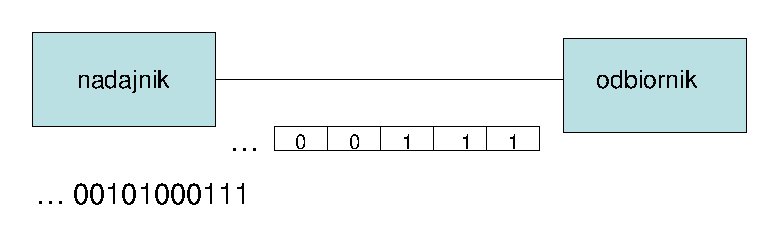
\includegraphics[width=9cm]{./wyklady/RS232_2_1.pdf}
			\item Równoległa - przesyłanie bitów słowa po przyporządkowanej każdemu bitowi linii transmisyjnej (bity przesyłane równolegle, słowa przesyłane szeregowo).\\
			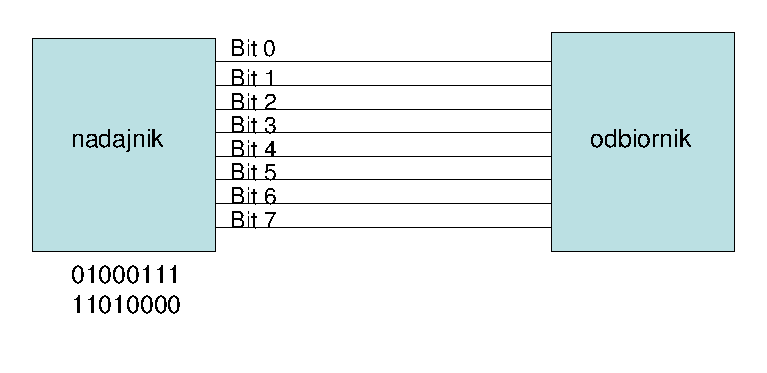
\includegraphics[width=9cm]{./wyklady/RS232_2_2.pdf}
		\end{itemize}
		\subsubsection{Definicje danych}
		\begin{itemize}
			\item "0" - 0V
			\item "1" - 12V
			\item Czas transmisji jednego bitu T - stały, nie większy niż czas propagacji.
			\item $\frac{1}{T}$ - liczba bitów przesyłana w jednostce czasu. Standardowe wartości 110, 150, 300, 600, 1200, 2400 ... [b/s]
			\item Impulsy rozeznające - sprawdzają stan bitów odebranych (następują co T, które narzuca nadawca).
		\end{itemize}
		\subsubsection{Jednostka informacyjna - znak}
		Jednostka informacji o ściśle określonym formacie. Odbiorca dysponuje impulsami próbkującymi, które rozpoznają stan sygnału (odpytują).\\
		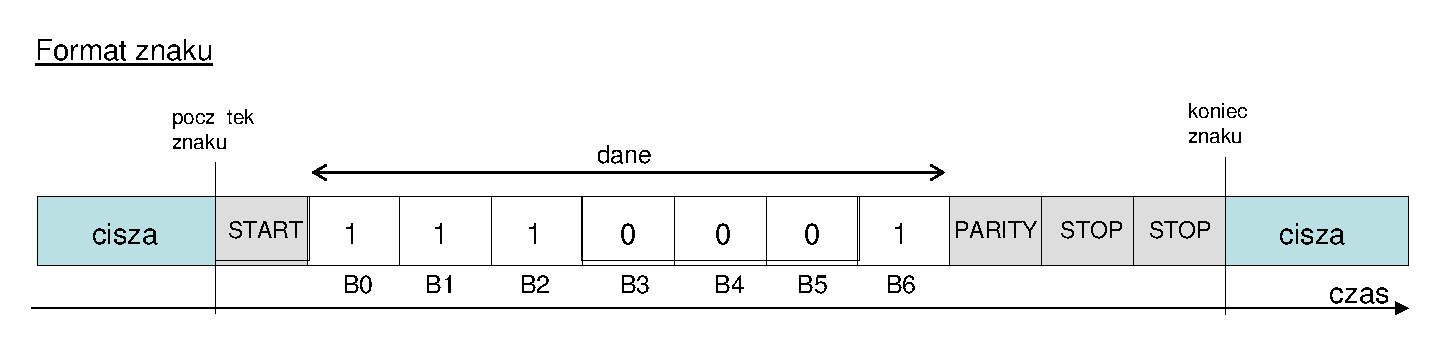
\includegraphics[width=10cm]{./wyklady/RS232_3_2.pdf}\\
		\subsubsection{Przekazywanie konfiguracji}
			Aby nadawca i odbiorca mogli się porozumieć i interpretować znaki w ten sam sposób, muszą zostać tak samo skonfigurowane. Innymi słowy, muszą posiadać ten sam takt nadawania.\\Metody:\\
			\begin{itemize}
				\item dodatkowe łącze
				\item jako element konfiguracji (wykorzystanie generatorów kwarcowych, synchronizm częstotliwościowy)
			\end{itemize}
			Nominalne położenie impulsu = ok. $\frac{1}{2}\times{T}$ - pośrodku, największe bezpieczeństwo próbkowania. Służą do tego układy korekcji fazy impulsu - liczniki, zliczają liczbę impulsów na wejściu i dają 1 na wyjściu.
		\subsubsection{Definicja znaku}
		\begin{itemize}
			\item \textbf{START} - bit kontrolny, znacznik początku (SOF - Start Of Frame) - jałowy z punktu widzenia przesyłanej informacji i służący jedynie w celu synchronizacji. START zapewnia $\frac{n}{2}$ jako stan licznika (fazy impulsu).
			\item \textbf{DANE} - 7-8 bitów (kiedyś też 5-6, obecnie już nieużywane), które są treścią znaku, począwszy od bitu najmniej znaczącego (LSB - least significant bit). Tym bitem jest B0.
			\item \textbf{PARITY} – bit kontroli poprawności znaku, służy jako zabezpieczenie informacji. Może, ale nie musi występować. Jednak decyzja o jego występowaniu ma charakter globalny - dotyczy każdego znaku w danej transmisji. Jego stan określa zasada:
			\begin{itemize}
				\item Kontrola parzystości (Even parity) - polega na sprawdzeniu liczby jedynek na polu danych i ustawieniu bitu kontrolnego na "1" w przypadku nieparzystej liczby jedynek lub na "0" w przypadku parzystej (uzupełnienie do parzystości).
				\item Kontrola nieparzystości (Odd parity) - polega na sprawdzeniu liczby zer na polu danych i ustawieniu bitu kontrolnego na "1" w przypadku nieparzystej liczby zer lub na "0" w przeciwnym przypadku.
				\item Brak kontroli (None)
			\end{itemize}
			Ten bit kontroli pozwala wykryć przekłamanie w transmisji danych pod warunkiem, ze liczba przekłamań jest nieparzysta.
			\item \textbf{STOP} – 1 lub 2 bity kontrolne, znacznik końca znaku.
		\end{itemize}
		\subsubsection{Konwencja nazewnicza rodzajów transmisji}
			[Ilość bitów danych][Rodzaj kontroli][Liczba bitów stopu]\\Przykłady:
			\begin{itemize}
				\item 7E2 - 7 bitów danych, kontrola parzystości, 2 bity stopu (10 bitów + START = 11 bitów)
				\item 8O1 - 8 bitów danych, kontrola nieparzystości, 1 bit stopu (11 bitów)
				\item 8N2 - 8 bitów danych, brak kontroli, 2 bity stopu (11 bitów)
			\end{itemize}
		\subsubsection{Rodzaje transmisji}
		\begin{itemize}
			\item \textbf{Synchroniczna} - elementy informacji wysyłane w takt zegara nadajnika. W ten sposób przesyłane są bity w ramach pojedynczej jednostki informacyjnej.
			\item \textbf{Asynchroniczna} - wysyłanie elementów informacji niesynchronizowane zegarem nadajnika. W ten sposób są wysyłane poszczególne jednostki - ich wprowadzanie nie jest sygnalizowany żadnym sygnałem, więc odstęp między nimi jest dowolny.\\
			Czas trwania bitu nazywa się \emph{odstępem jednostkowym} i oznaczamy go $t_{b}$. Jego odwrotność ($f=\frac{1}{t_{b}}$) określa szybkość transmisji w bodach, gdzie 1 [bd] = 1 [bit/s].
		\end{itemize}
		\subsubsection{Transmisja w RS-232}
		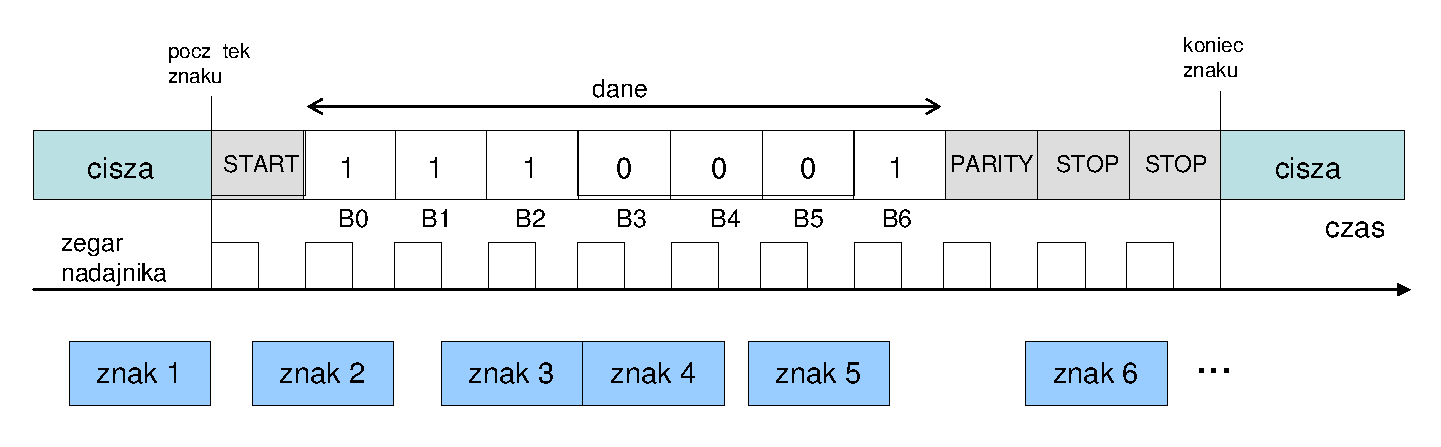
\includegraphics[width=9cm]{./wyklady/RS232_4_1.pdf}
		\begin{itemize}
			\item Synchroniczne wysyłanie bitów
			\item Asynchroniczne wysyłanie znaków
			\begin{itemize}
				\item Polega na wysyłaniu pojedynczych znaków, które mają ścisłe określony format.
				\item Brak sygnału zegarowego określającego momenty wysyłania znaków.
				\item Odstępy między znakami nieokreślone.
			\end{itemize}
		\end{itemize}
		\subsubsection{Tryby transmisji}
		\begin{itemize}
			\item \textbf{Simpleksowa} - jednokierunkowa, z nadajnika do odbiornika.
			\item \textbf{Półdupleksowa} (HDX) - dwukierunkowa, niejednoczesna (w danej chwili czasu jedno urządzenia jest nadajnikiem, a drugie odbiornikiem). Zakłada istnienie tylko jednej linii transmisyjnej. Wymaga konfiguracji (informacja, kto kiedy nadaje).
			\item \textbf{Dupleksowa} (FDX) - dwukierunkowa, jednoczesna (w danej chwili czasu oba urządzenia mogą spełniać rolę nadajnika lub odbiornika). Brak konieczności sprawdzania czy łącze jest wolne oraz mechanizmu rezerwacji łącza.
		\end{itemize}
	\subsection{Komunikacja DTE-DCE - sygnały w porcie RS-232}
	Komunikacja dwóch stacji DTE przez komutowane łącze telefoniczne.\\
	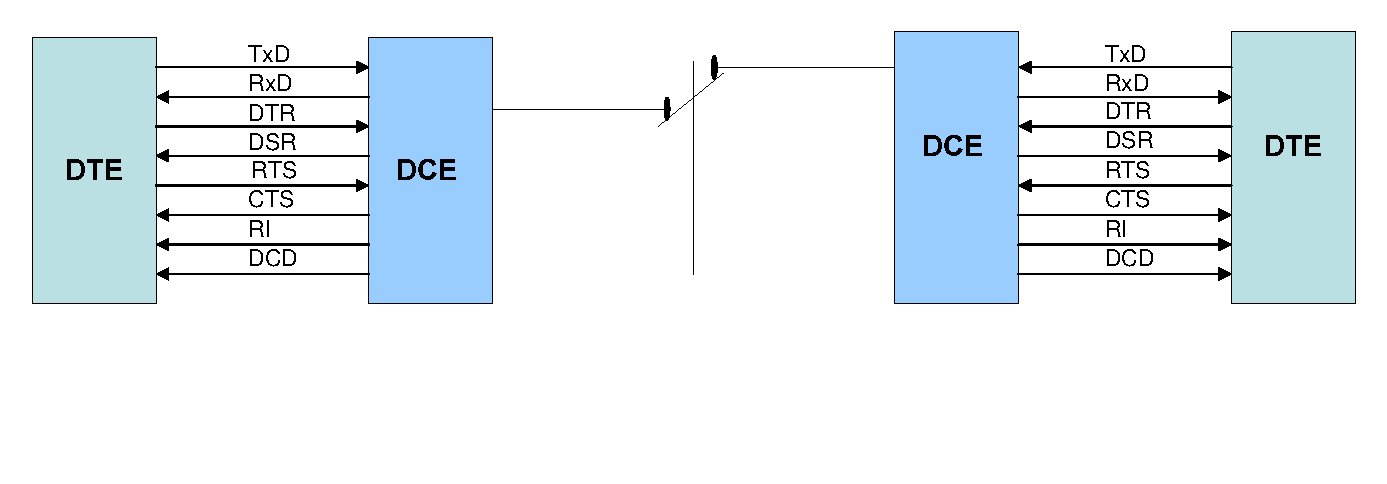
\includegraphics[width=12cm]{./wyklady/RS232_6_1.pdf}\\
	\begin{table}[h]
		\begin{tabular}{|c|c|c|c|c|}
			\hline
			\multicolumn{5}{|c|}{\textbf{Urządzenia}}                        \\ \hline
			\multicolumn{1}{|c|}{DTE} & \multicolumn{2}{|c|}{Data Terminal Equipment}      & \multicolumn{2}{|c|}{Komputer}           \\ \hline
			\multicolumn{1}{|c|}{DCE} & \multicolumn{2}{|c|}{Data Communication Equipment} & \multicolumn{2}{|c|}{Modem}              \\ \hline
			\multicolumn{5}{|c|}{\textbf{Linie} (sygnały)}                   \\ \hline
			\textbf{Skrót} & \textbf{Nazwa}	   & \textbf{Znaczenie} & \textbf{Przeznaczenie} & \textbf{Kierunek} \\ \hline
			TxD & Transmitted Data             & Dane nadawane      & Linia danych		& Wyjście	\\ \hline
			RxD & Received Data                & Dane odbierane     & Linia danych		& Wejście	\\ \hline
			DTR & Data Terminal Ready          & Gotowość DTE       & Linia kontrolna	& Wyjście	\\ \hline
			DSR & Data Set Ready               & Gotowość DCE       & Linia kontrolna	& Wejście	\\ \hline
			RTS & Request to Send              & Żądanie nadawania  & Linia kontrolna	& Wyjście	\\ \hline
			CTS & Clear To Send                & Zgoda na nadawanie & Linia kontrolna	& Wejście	\\ \hline
			RI  & Ring Indicator               & Wskaźnik wywołania & Linia kontrolna   & Wejście	\\ \hline
			DCD & Data Carrier Detected        & Wykrycie nośnej    & Linia kontrolna   & Wejście	\\ \hline
			SG  & Signal Ground                & Masa sygnałowa     & Masa				& ------	\\ \hline
		\end{tabular}
	\end{table}
		\subsubsection{Fazy pracy układu}
		\begin{itemize}
			\item Tryb nawiązywania połączenia
			\item Tryb transmisji danych (wtedy nas interesują dupleksy i inne)
		\end{itemize}
		\subsubsection{Linie w złączu RS-232}
		\begin{itemize}
			\item Linie danych: TxD, RxD
			\item Linie kontrolne: DTR, DSR, RTS, CTS, RI, DCD
		\end{itemize}
	\subsection{Połączenie bezmodemowe DTE-DTE}
	Przykład połączenia dla transmisji dupleksowej.\\
	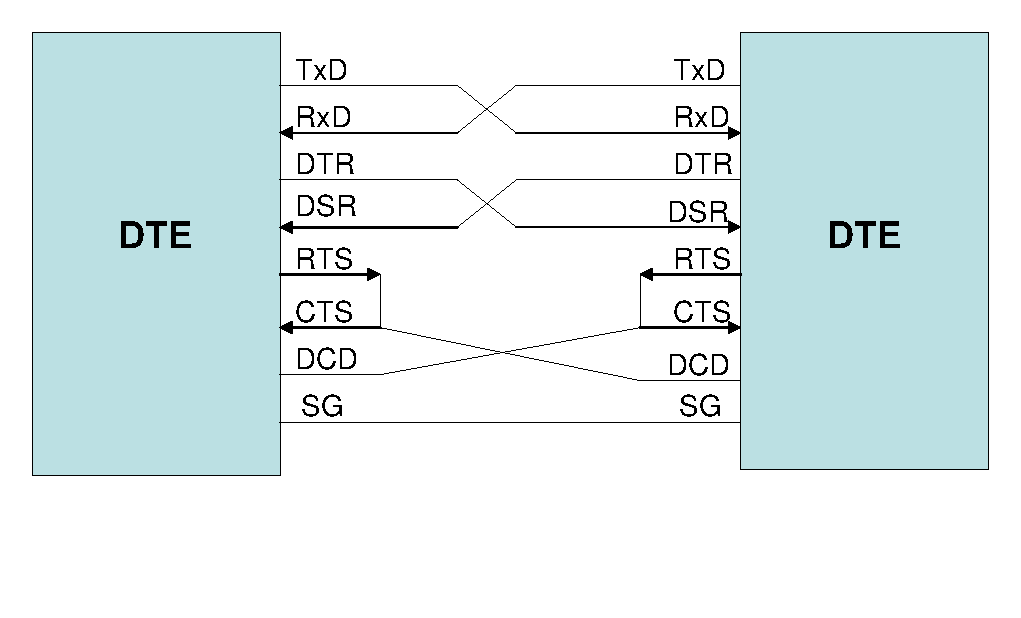
\includegraphics[width=9cm]{./wyklady/RS232_7_1.pdf}
	\begin{itemize}
		\item PG, SG - masa
		\item TxD, RxD - dane
		\item RTS, CTS, DCD, DSR, DTR - sterowanie
	\end{itemize}
	\subsection{Kontrola transmisji: handshake i protokół XON/XOFF}
		\subsubsection{Handshake}
		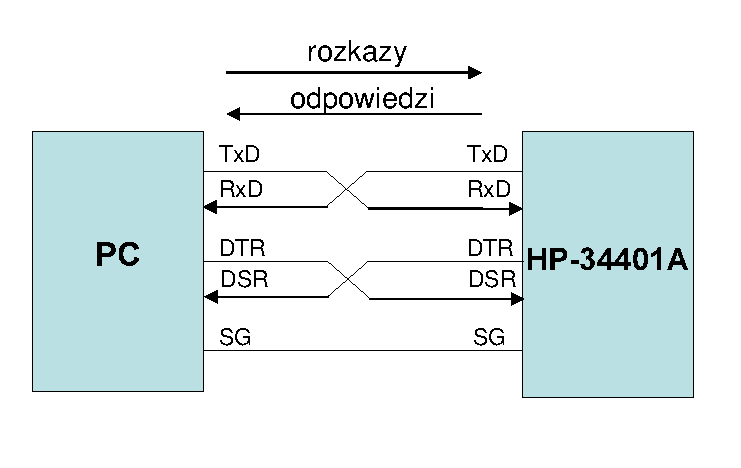
\includegraphics[width=9cm]{./wyklady/RS232_9_1.pdf}
		\begin{itemize}
			\item DTR = 1 - zgoda na nadawanie
			\item DTR = 0 - brak zgody na nadawanie
			\item DTR informuje, czy bufor jest zapełniony. DSR sprawdza go u partnera przed wysłaniem dalszych danych.
			\item Analogiczna sytuacja, kiedy podłączone są RTS i CTS zamiast DTR i DSR. RTS wystawia informację, CTS sprawdza.
		\end{itemize}
		\subsubsection{Protokół XON/XOFF}
		Występuje przy wymianie informacji w trybie dupleksowym. Umożliwia blokowanie i odblokowywanie transmisji danych. Np. drukarka - gdy skończy się papier w trakcie drukowania, przesył jest blokowany, Gdy użytkownik uzupełni papier, transmisja jest wznawiana. Taki protokół XON/OFF nazywany jest programowym (software XON/OFF). {\small Rozwiązanie hardware to transmisja półdupleksowa za pośrednictwem sygnałów w kanale wtórnym.}\\
		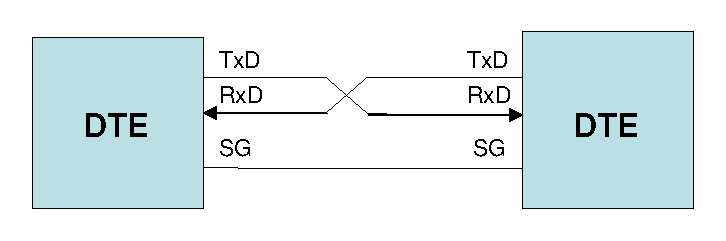
\includegraphics[width=9cm]{./wyklady/RS232_9_2.pdf}
		\begin{itemize}
			\item XON – ASCII 19 (CTRL-S)
			\item XOFF – ASCII 17 (CTRL-Q)
		\end{itemize}
	\subsection{Parametry elektryczne sygnałów}
	Poniżej przestawiono schemat "obwodu stykowego" złożonego ze źródła sygnału, toru transmisyjnego i odbiornika. Parametry zdefiniowano przy założeniu, że szybkość transmisji nie przekracza 20 kbd.
	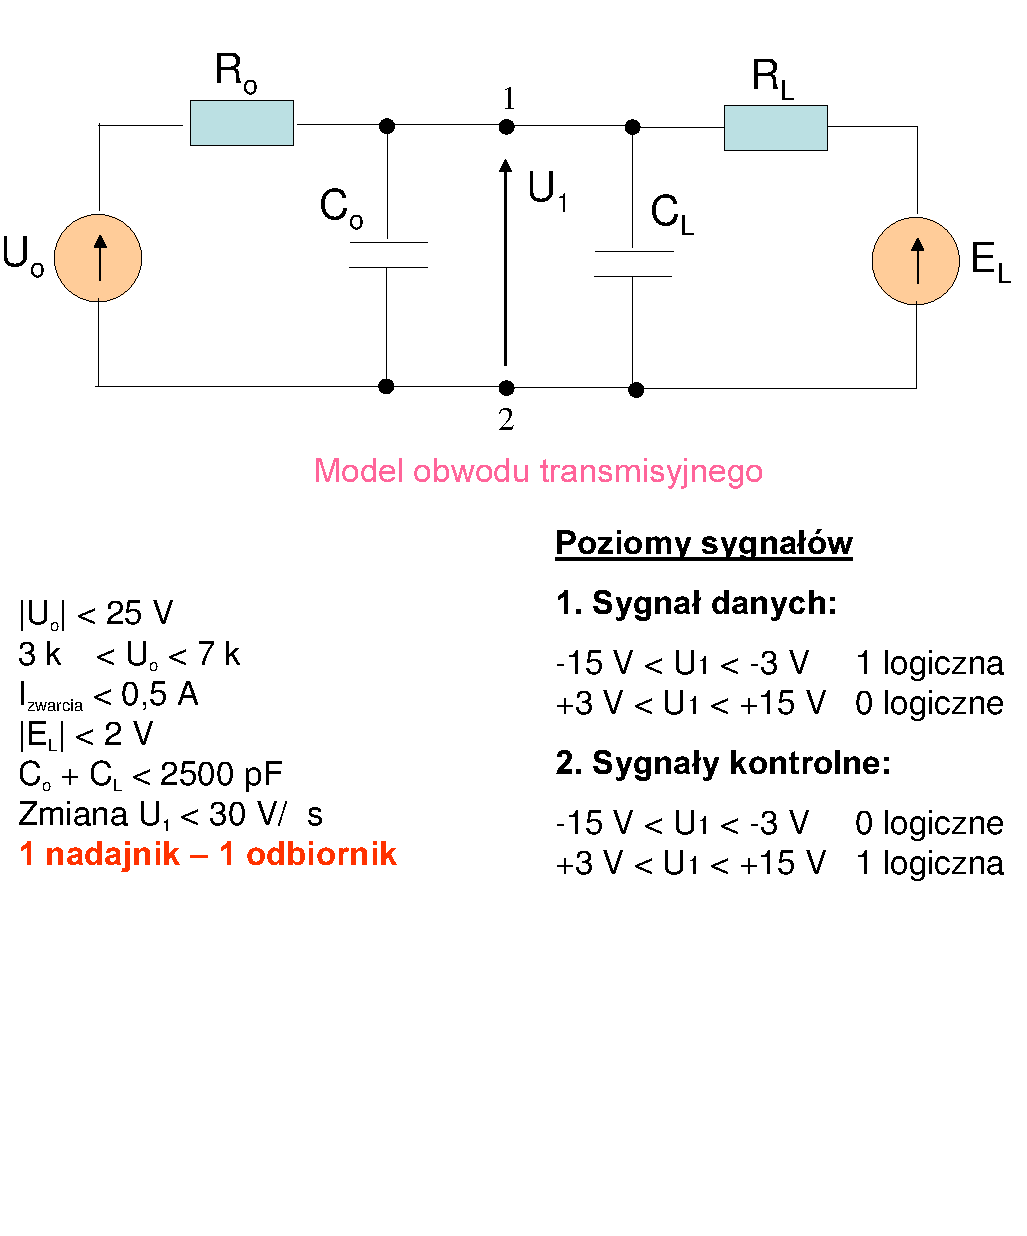
\includegraphics[width=9cm]{./wyklady/RS232_10_1.pdf}\\
	Na rysunku powyżej: kiloomy oraz mikrosekundy.\\
	Wada: jest to obwód represyjny, da się go silnie zakłócić poprzez różnicę potencjałów pomiędzy masami.
	\subsection{Standardy RS-423, RS-422, RS-485}
	Niesymetryczna przesyłanie danych w RS-232C ogranicza szybkość i odległość transmisji, a ponadto nie jest zabezpieczone przed zakłóceniami zewnętrznymi. Aby to polepszyć wymyślono inne standardy.
		\subsubsection{RS-423A}
		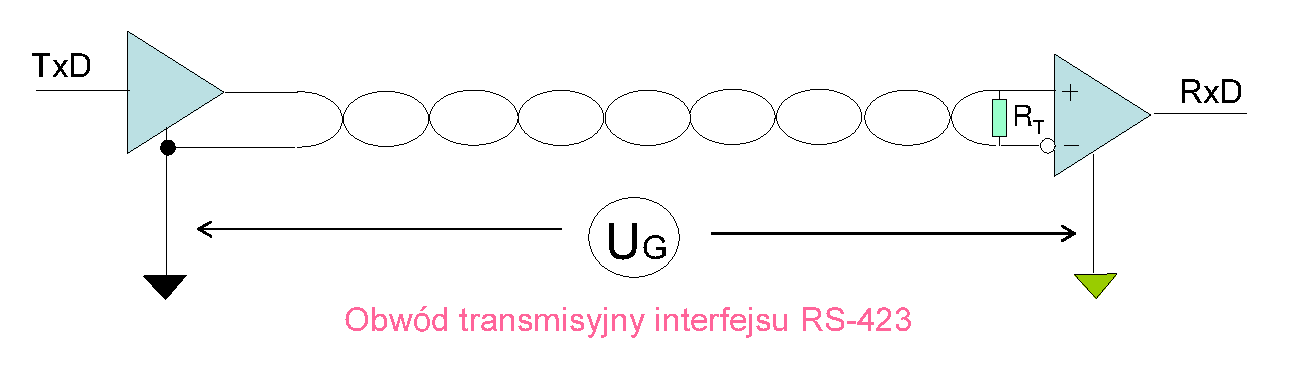
\includegraphics[width=9cm]{./wyklady/RS232_12_1.pdf}
		\begin{itemize}
			\item szybkość do 100 kbd (przy zasięgu do 30 m)
			\item zasięg do 1200 m (przy szybkosci do 3 kbd)
		\end{itemize}
		Standard RS-423A określa elektryczną charakterystykę napięciowego obwodu transmisyjnego złożonego z niesymetrycznego nadajnika oraz symetrycznego (różnicowego) odbiornika. Takie obwody stosuje się do przesyłania sygnałów binarnych pomiędzy DTE i DCE, które reprezentują dane lub funkcje sterujące.\\
		Zastosowanie różnicowego obciążenia pozwala na znaczne zmniejszenie wpływu napięcia wspólnego $U_{G}$ powstałego na wskutek różnicy potencjałów masy nadajnika i odbiornika, jak również przesłuchów między nimi.\\
		Standard wymaga aby dla każdego kierunku transmisji istniał przynajmniej jeden niezależny przewód powrotny.\\
		Typowa prędkość wynosi 100 kb/s przy odległości do 30 m.
		\subsubsection{RS-422A}
		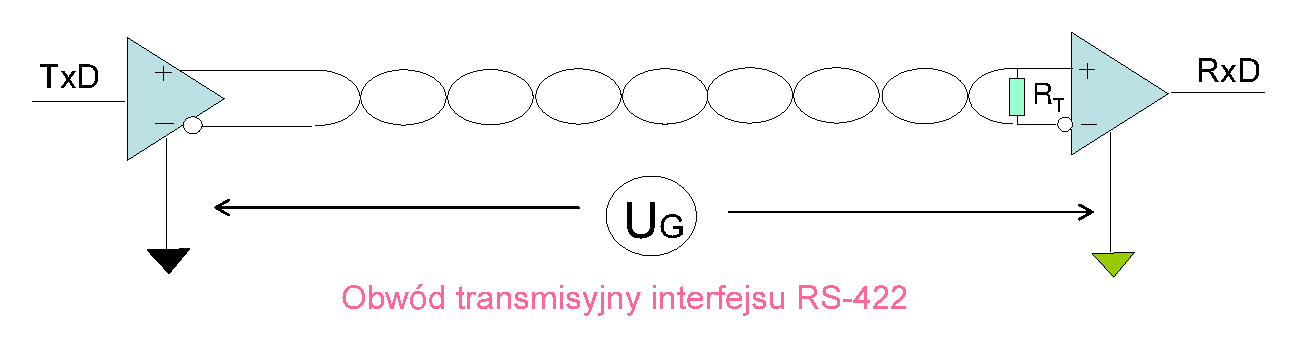
\includegraphics[width=9cm]{./wyklady/RS232_12_2.pdf}
		\begin{itemize}
			\item szybkość do 10 Mbd (przy zasięgu do 100 m)
			\item zasięg do 1200 m (przy szybkości 100 kbd)
		\end{itemize}
		Wykorzystuje pełną symetryzację łącza, zapewnia szybka transmisję w obecności zakłóceń. Standardy RS-423 oraz RS-485 określają symetryczny, zrównoważony system transmisji danych złożony z:
		\begin{itemize}
			\item różnicowego nadajnika
			\item dwuprzewodowego zrównoważonego toru przesyłowego
			\item odbiornika o różnicowym obwodzie wejściowym.
		\end{itemize}
		Standard RS-422A nie wprowadza ograniczeń na minimalną i maksymalną częstotliwość, a jedynie na zależność między szybkością zmian sygnału, a czasem trwania bitu.
		\subsubsection{RS-485A}
		Standard RS-485A jest rozwinięciem RS-422. Łącze RS-485A jest również zrównoważone i symetryczne, przy czym dopuszcza się nie tylko wiele odbiorników, ale i wiele nadajników podłączonych do jednej linii. Nadajniki muszą być trójstanowe.\\
		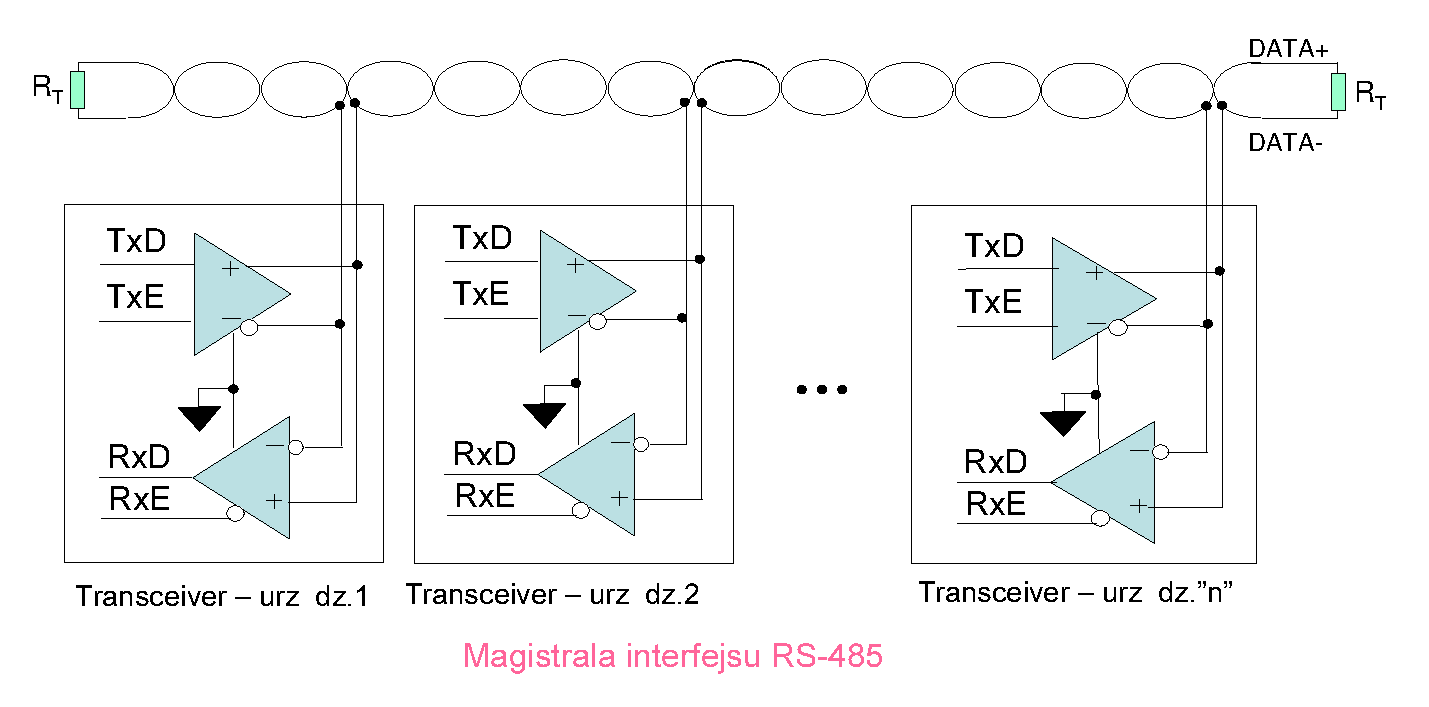
\includegraphics[width=10cm]{./wyklady/RS232_13_1.pdf}
	\subsection{Systemy komunikacyjne oparte na łączu znakowym}
		\subsubsection{System oparty na szeregowym łączu znakowym}
		Podłączenie urządzenia RS-232 do portu COM z pom. int. RS-485\\
		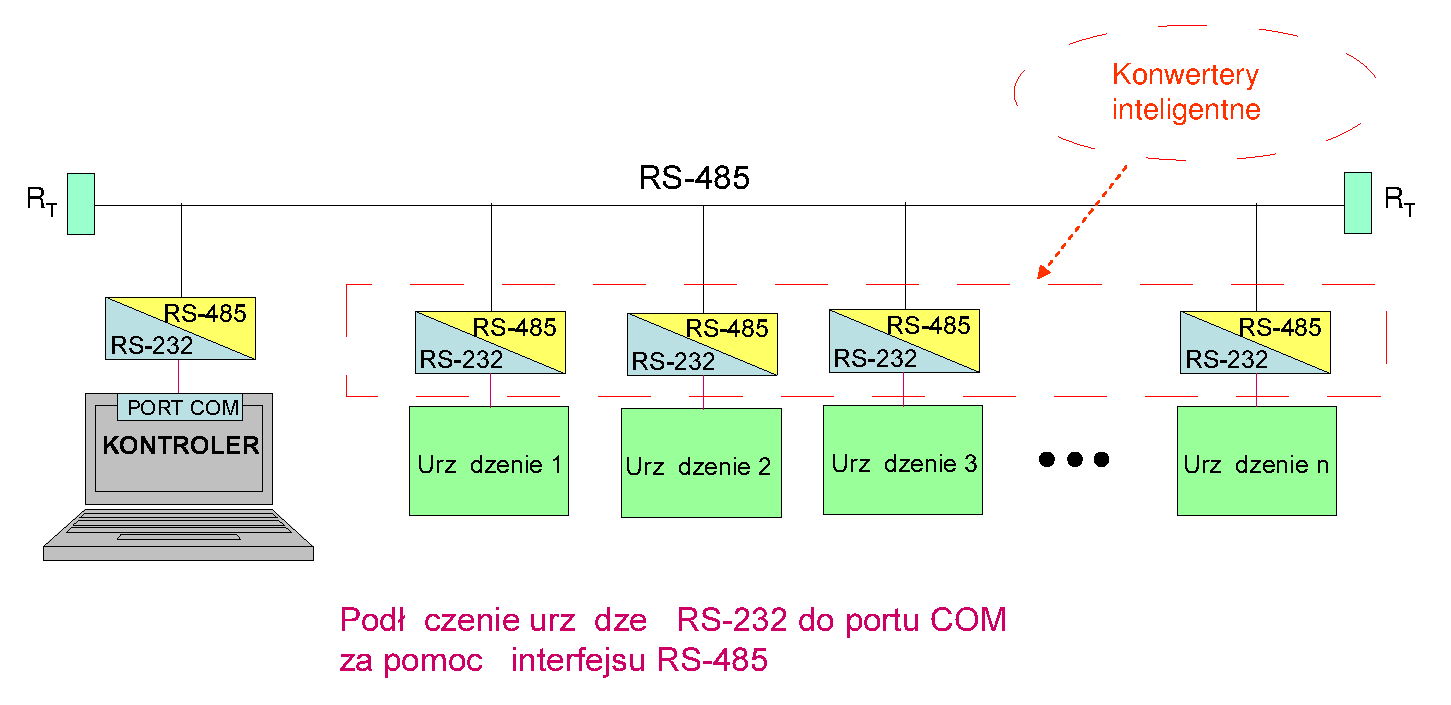
\includegraphics[width=9cm]{./wyklady/RS232_14_1.pdf}\\
		R\tiny T\normalsize - Rezystory zabezpieczające przed niekorzystnym odbiciem fali (tzw. Terminatory).\\
		\textbf{Problem}: dostęp do magistrali kontrolera i urządzeń systemu\\
		\textbf{Rozwiązanie}: Implementacja protokołu komunikacyjnego (warstwa łącza danych). Komputer zarządza innymi urządzeniami w całym systemie. Do zbudowania tego wystarczają proste przejściówki do zmian sygnałów.\\
		\textbf{Komunikacja}:
		\begin{itemize}
			\item Selekcja urządzenia kontrolującego (master) - generuje on rozgłoszenie (broadcast) do wszystkich urządzeń i zbiera dane.
			\item Selekcja urządzenia odbierającego - konieczna gdy wiele urządzeń chce przesłać odpowiedź do mastera, co może powodować konflikt.
			\begin{itemize}
				\item nadanie identyfikatorów (adresacja urządzeń)
				\item zastosowanie przejściówek - są inteligentne i odpowiadają za dostęp do urządzenia.
			\end{itemize}
		\end{itemize}
		\subsubsection{System oparty na łączu znakowym}
		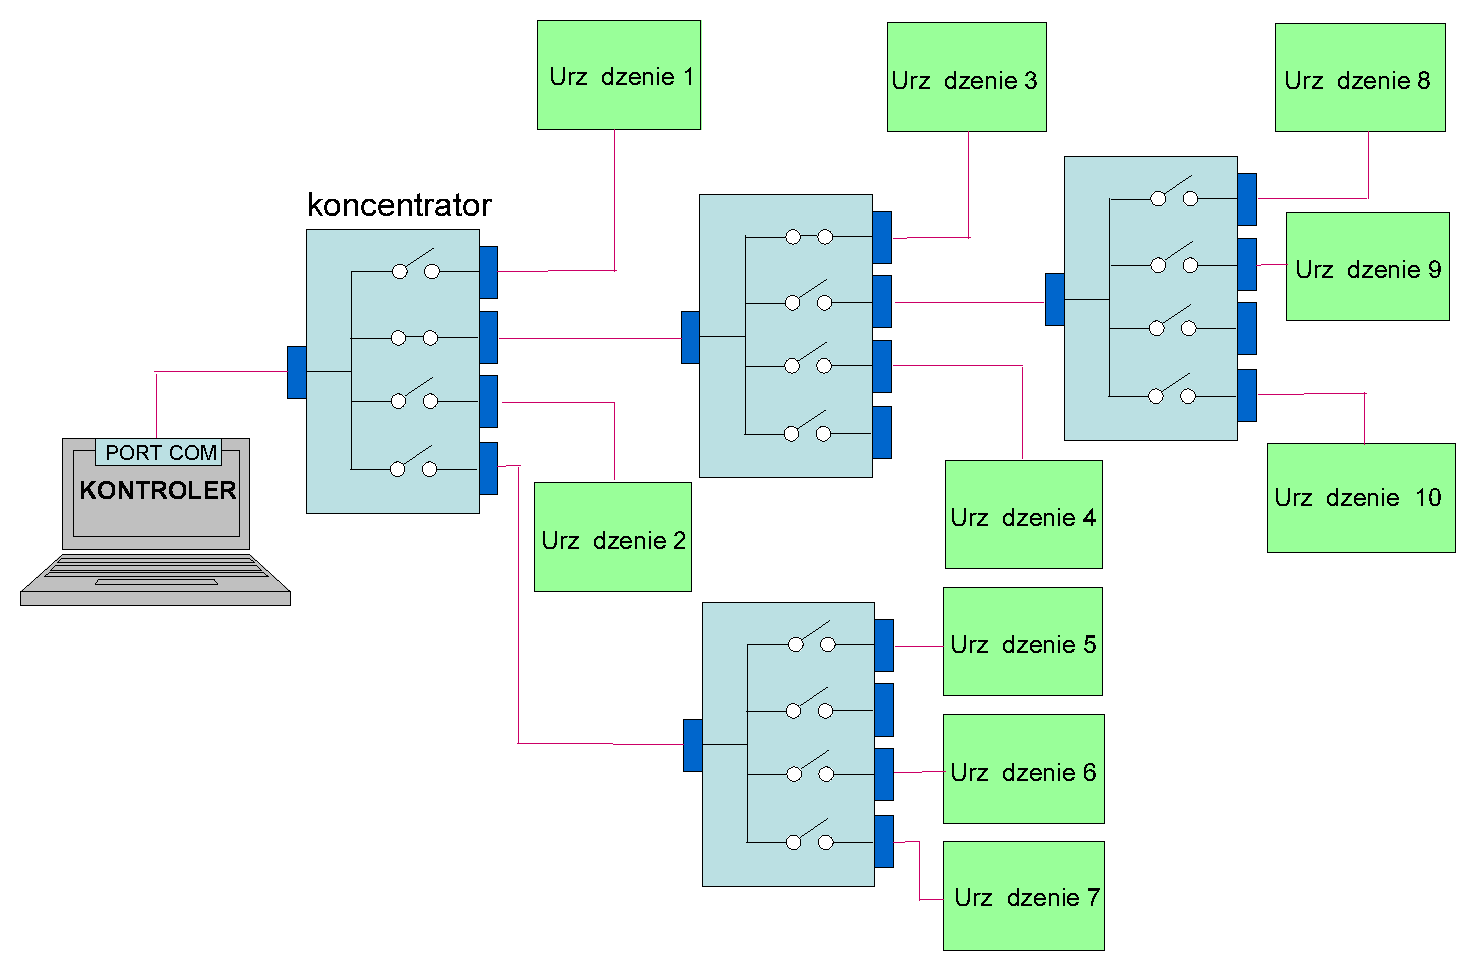
\includegraphics[width=10cm]{./wyklady/RS232_15_1.pdf}\\
		Koncentrator zawiera 4 klucze portu RS. Dostęp jest tylko do jednego wyjścia naraz.\\
		\textbf{Kaskadowe połączenie} - przełącznik podłączony do przełącznika. Pojawia się problem wyboru drogi do urządzenia, która musi być znana. Koncentratory muszą mieć informacje o \textbf{mapie urządzeń}.
	\subsection{System MODBUS}
		Interfejs MODBUS został opracowany w firmie Modicon i jest przyjętym standardem w dla asynchronicznej, znakowej wymiany informacji pomiędzy urządzeniami systemów pomiarowo-kontrolnych.
		\subsubsection{Charakterystyka}
			\begin{itemize}
				\item Reguła dostępu do łącza na zasadzie Master-Slave. 
				\item Zabezpieczenie przesyłanych komunikatów przed błędami
				\item Potwierdzenie wykonania rozkazów zdalnych i sygnalizacja błędów
				\item Mechanizmy zabezpieczające przed zawieszeniem systemu
				\item Wykorzystanie asynchronicznej transmisji znakowej zgodnej z RS-232C
			\end{itemize}
		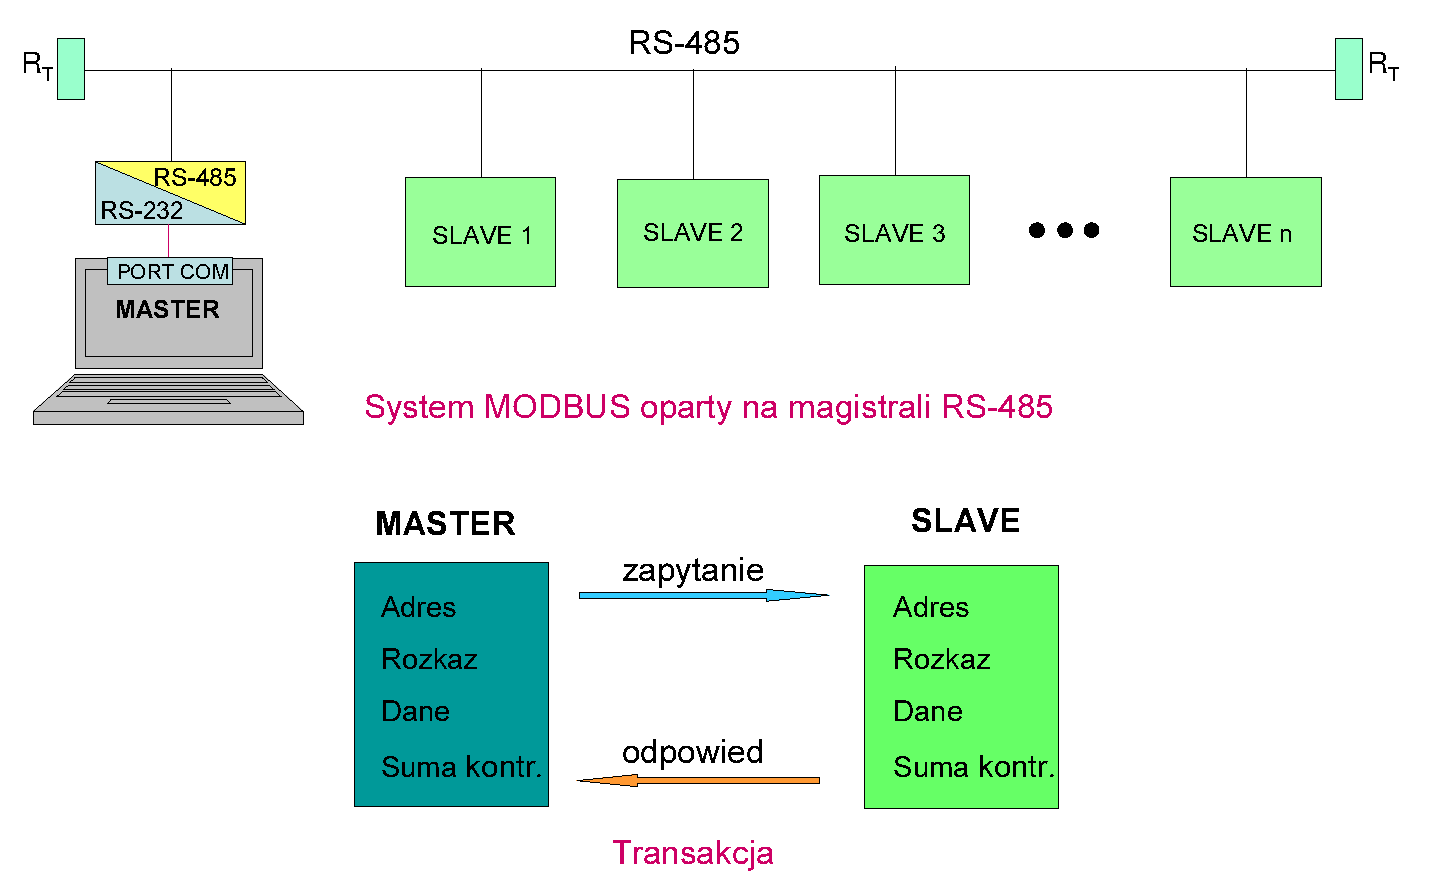
\includegraphics[width=9cm]{./wyklady/RS232_16_1.pdf}\\
		\subsubsection{Transakcja}
		Jedno urządzenie może inicjować transakcje (master), a pozostałe (slave) odpowiadają jedynie na zapytania mastera. Transakcja składa się z polecenia (query) wysyłanego z master do slave oraz z odpowiedzi (response) przesyłanej ze slave do master. Odpowiedź zawiera dane żądane przez master lub potwierdzenie realizacji jego połączenia. Wykrycie końca kończy fazę w której następuje przekazanie łącza masterowi.\\
		\subsubsection{Format wiadomości}
		Dotyczy zarówno poleceń jednostki nadrzędnej, jak i odpowiedzi podrzędnych.
		\begin{itemize}
			\item Adres
			\item Kod funkcji reprezentujący rozkaz, pierwszy bit rozkazu oznacza jego rodzaj. 0 - normalny, 1 - szczególny.
			\item Dane
			\item Kontrola błędów (dla pracy w warunkach przemysłowych)
		\end{itemize}
		W przypadku odpowiedzi odpowiednio w polach znajdują się:
		\begin{itemize}
			\item Adres (swój, slave'a, do kontroli poprawności)
			\item Pole potwierdzenia realizacji rozkazu
			\item Dane żądane przez master
			\item Kontrola błędów
		\end{itemize}
		\subsubsection{Rodzaje transakcji}
			\begin{itemize}
				\item \textbf{Adresowana} - przeznaczona dla pojedynczej jednostki slave
				\item \textbf{Rozgłoszeniowa} (broadcast) - wysyłana do wszystkich jednostek podrzędnych. Na ten rodzaj polecenia jednostki nie przesyłają odpowiedzi.
			\end{itemize}
		\subsubsection{Rodzaje odpowiedzi}
			\begin{itemize}
				\item \textbf{Normalna} - w przypadku poprawnego wykonania polecenia.
				\item \textbf{Szczególna} - jeżeli slave wykryje błąd przy odbiorze wiadomości lub nie jest w stanie wykonać polecenia, to przygotowuje specjalny komunikat o wystąpieniu błędu i przesyła jako odpowiedź. W przypadku tej wiadomości jest ona \textbf{powiększona} o 128 - miejsce na kod błędu.
			\end{itemize}
		\subsubsection{Parametry protokołu}
			\begin{itemize}
				\item Reguła dostępu do łącza: Master-Slave
				\item Zakres adresów: 1 - 247 (identyfikatory slave'ów)
				\item Adres rozgłoszeniowy: 0, rozpoznawany przez wszystkie slave'y
				\item Kontrola błędów: LRC/CRC, ograniczenie czasowe odpowiedzi
				\item Wymagana ciągłość przesyłania znaków w ramce
			\end{itemize}
		\subsubsection{Ramka w systemie MODBUS}
			W systemie MODBUS wiadomości są zorganizowane w ramki o określonym początku i końcu. Umożliwia do odbiornikowi odrzucenie ramek niekompletnych i sygnalizację błędów.
		\subsubsection{Rodzaje transmisji ramek}
			\begin{itemize}
				\item ASCII
				\item RTU
			\end{itemize}
		\subsubsection{Ramka w trybie ASCII}
			Każdy bajt wiadomości przesyłany jest w postaci dwóch znaków ASCII. Zaletą tego rozwiązania jest to, że pozwala na długie odstępy między znakami (1 s) bez powodowania błędów.\\\\\textbf{Format znaku}\\
			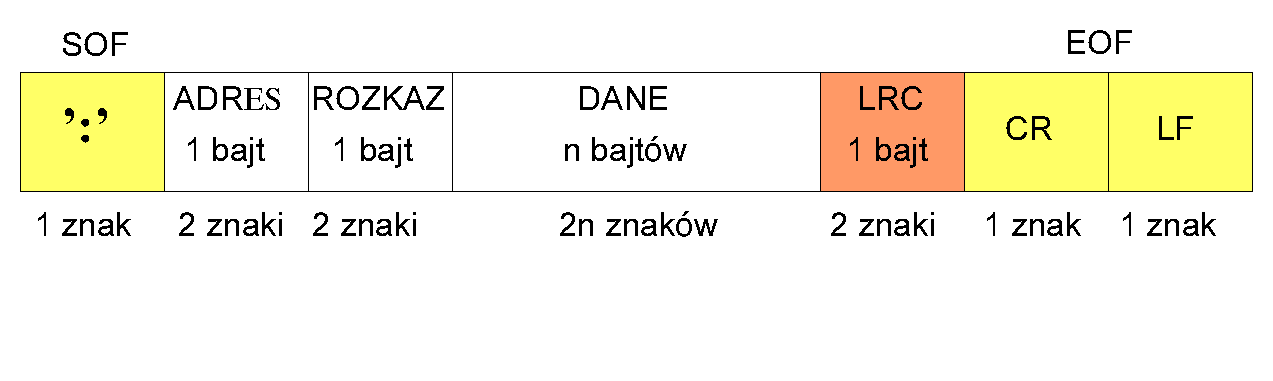
\includegraphics[width=10cm]{./wyklady/RS232_18_1.pdf}
			\begin{itemize}
				\item System kodowania: heksadecymalny, znaki ASCII 0-9, A-F. Jeden znak heksadecymalny zawarty jest w każdym znaku ASCII wiadomości.
				\item Jednostka informacyjna: ograniczona znakami start (na początku) i stop (na końcu), 10-bitowa.
				\item Znacznikiem początku ramki jest znak dwukropka (":" - ASCII 3Ah).
				\item Dopuszczalne znaki dla pozostałych pól (poza znacznikiem końca ramki) to 0-9, A-F.
				\item Pole funkcji: dwa znaki w trybie ASCII
				\item Podsumowując: wykorzystujemy 2 znaki heksadecymalne do przesyłu 1go znaku ASCII. Dzielimy ten na dwie części i przesyłamy w dwóch pakietach po 10 bitów.
				\item Urządzenie po wykryciu znacznika początku sprawdza czy pole adresowe zawiera jego własny adres. Jeżeli tak, to odczytuje zawartość pola funkcji i pola danych.
				\item Pole kontrolne LRC (1-bitowe) zabezpiecza część informacyjną. Sumuje cześć informacyjną bajtu i uzupełnia do 2.
				\item Ramka kończy się przesłaniem dwóch znaków: CR i LF.
				\item Ramkę kończy przerwa czasowa trwająca co najmniej $3.5\times$(długości znaku)
				\item Ramki muszą być przesyłane w postaci ciągłej, tzn. odstęp między kolejnymi znakami tworzącymi ramkę nie może być większy niż $1.5\times$(długości znaku).
			\end{itemize}
			Stosowane jest zabezpieczenie części informacyjnej ramki kodem LRC (Longitudinal Redundancy Check).
		\subsubsection{Ramka w trybie RTU}
			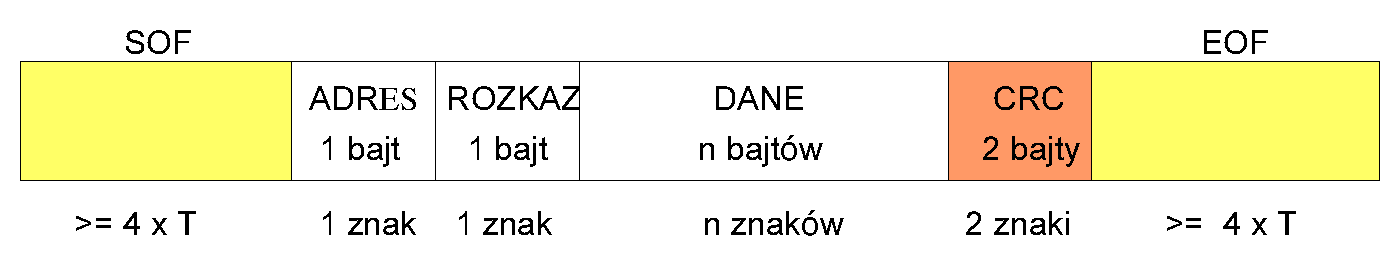
\includegraphics[width=10cm]{./wyklady/RS232_18_2.pdf}\\
			W trybie RTU wiadomości zaczynają się odstępem czasowym trwającym minimum $3.5\times$(\emph{czas trwania pojedynczego znaku}), w którym panuje cisza na łączu (można to zrealizować np. przez odmierzanie czasu trwania znaku przy zadanej na łączu szybkości bodowej).
			\begin{itemize}
				\item Pierwszym polem informacyjnym jest adres urządzenia
				\item Dopuszczalne znaki w ramach pól ramki: 0-9, A-F
				\item Zakres kodów operacji: 1 - 255
				\item Urządzenia stale monitorują magistralę. Jak adres odebrany w wiadomości zgadza się z ich własnym, to lecą dalej.
				\item Ramkę kończy przerwa czasowa trwająca co najmniej $3.5\times$(długości znaku)
				\item W przypadku gdy nowa wiadomość pojawia się przed upływem niezbędnej przerwy to będzie ona potraktowana jako kontynuacja poprzedniej wiadomości. Doprowadzi to do błędu sumy kontrolnej.
				\item Ramki muszą być przesyłane w postaci ciągłej, tzn. odstęp między kolejnymi znakami tworzącymi ramkę nie może być większy niż $1.5\times$(długości znaku).
				\item Przekroczenie odstępu powoduje uznanie ramki za niekompletną i błędną.
				\item Kontrola danych typu CRC - 2-bajtowe, silniejsze niż LRC.
			\end{itemize}
		\subsubsection{Warstwa fizyczna}
		\begin{itemize}
			\item Asynchroniczna transmisja znakowa
			\item Formaty znaków
			\begin{itemize}
				\item Tryb ASCII: 7E1, 7O1, 7N2
				\item Tryb RTU: 8E1, 8O1, 8N2
			\end{itemize}
			\item Szybkość: od 1200 bd do 19200 bd
			\item Rodzaj łącza:
			\begin{itemize}
				\item Magistrala RS-485
				\item Multipleksowany RS-232
			\end{itemize}
			\item Rodzaj transmisji (zależny od łącza):
			\begin{itemize}
				\item różnicowa dla RS-485
				\item odniesiona do masy dla RS-232
			\end{itemize}
		\end{itemize}
	\subsection{Kontroler RS-232 w komputerze PC}

%USB
% !TeX spellcheck = pl_PL

\section{USB – Uniwersalny interfejs szeregowy}
	\subsection{Zalety}
	\begin{itemize}
		\item Podłączenie dużej liczby różnorodnych urządzeń
		\item Automatyczne wykrywanie włączenia urządzenia do systemu oraz jego odłączenia
		\item Przeprowadzanie wszystkich operacji konfiguracyjnych, w tym instalacji sterownika, bez udziału użytkownika
		\item Szybka transmisja
		\item Zasilanie urządzenia bezpośrednio z portu
	\end{itemize}
	\subsection{Parametry}
	Dla USB 1.1 oraz 2.0
	\begin{itemize}
		\item Szybkość transmisji: 12 Mb/s (1.1), 480 Mb/s (2.0)
		\item Złożoność kontrolera w stacji host: 10000 bramek
		\item Złożoność kontrolera w urządzeniu: 1500 do 2000 bramek
	\end{itemize}
	\subsection{Charakterystyka systemu USB}
		\subsubsection{Podstawowe właściwości interfejsu USB}
		\begin{itemize}
			\item \textbf{Gorące podłączenie} - włączanie/wyłączanie urządzeń bez wyłączania systemu oraz konfiguracja bez udziału użytkownika.
			\item \textbf{Jeden typ złącza} - złącze typu A w koncentratorze i B w urządzeniu (dwa kontakty linii danych oraz dwa zasilania).
			\item \textbf{Duża liczba podłączanych urządzeń} - moduły komunikacyjne, jak hub czy koncentrator, posiadają kilka portów USB oraz umożliwiają łączenie kaskadowe w celu rozszerzenia liczby portów do podłączanie urządzeń. W ten sposób można uzyskać wielopoziomową gwieździstą strukturę.\\Ostatecznie do USB można podłączyć maksymalnie \textbf{127} urządzeń.
			\item \textbf{Różne szybkości transmisji}
			\begin{itemize}
				\item Mała (\emph{low speed}): 1,5 Mb/s
				\item Pełna (\emph{full speed}): 12 Mb/s
				\item Wysoka (\emph{high speed}): 480 Mb/s
			\end{itemize}
			\item \textbf{Zasilanie} - USB posiada własny system dystrybucji zasilania: minilanie dostarcza 4.7 V/100 mA, maksymalnie 500 mA. Przy braku aktywnosci na magistrali przez 3s urządzenia przechodzą w tryb zmniejszonego poboru prądu (SUSPEND), gdzie moga pobierać maksymalnie 500 $\mu A$. Wyjscie z tego trybu jest możliwe poprzez inicjatywę hosta bądź urządzenia (\emph{remote wake-up})
			\item \textbf{Protokół komunikacyjny, detekcja błędów} - obowiązuje złożony, pakietowy protokół k. z kontrolą poprawności przesyłu. Żądania przesłania danych (\emph{transfer}) dzielone są na transakcje , które z kolei złożone są z pakietów: kontrolnego, danych i potwierdzenia. Pakiety są zabezpieczone sumą kontrolną. W przypadku wykrycia błędu jest możliwe powtórzenie transakcji.
			\item \textbf{Transfery USB} - 4 typy transferów:
				\begin{itemize}
					\item Kontrolny (control transfer)
					\item Masowy (bulk transfer)
					\item Przerwaniowy (interrupt transfer)
					\item Izochroniczny (isochronous transfer)
				\end{itemize}
			\item \textbf{Niski koszt} - nieduża złożoność układów interfejsowych
			\item \textbf{Schemat blokowy systemu USB}\\
			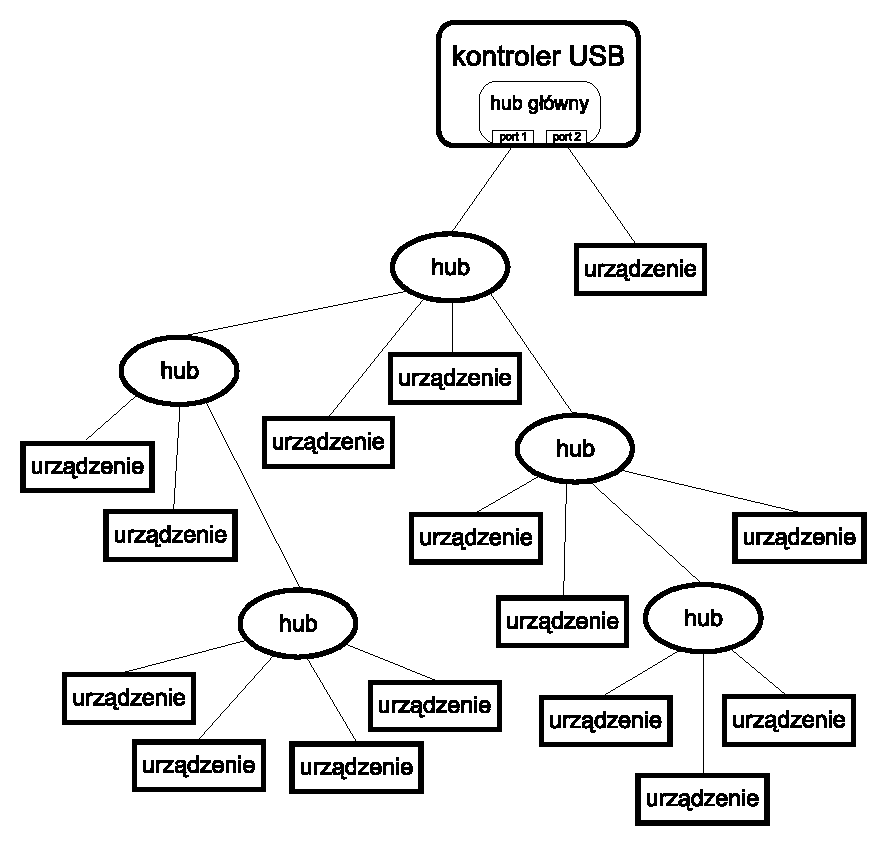
\includegraphics[width=10cm]{./wyklady/USB_6_1.pdf}
		\end{itemize}
		\subsubsection{Środowisko sygnałowe}
		Łącze transmisyjne oparte jest na obwodzie różnicowym. Różnicowy nadajnik jest połączony z różnicowym odbiornikiem przez parę przewodów.\\
		W przypadku transmisji wolnej wystarcza para nieskręcana i nieekranowana, natomiast transmisja pełna lub wysoka wymaga pary skręcanej i ekranowanej.\\
		Zasilanie jest przekazywane przewodami $V_{cc} (+5V)$ oraz $GND$ (masa).\\
		Trójstanowy nadajnik można zablokować sygnałem OE, co oznacza blokadę portu. Wówczas wyjście nieodwracające (D+) i odwracające (D-) przy zablokowanym nadajniku zostają na potencjale masy (patrz rezystory 15k).\\
		Wzmacniacze odniesione do masy monitorują napięcie na liniach D+ i D-.\\\\
			\textbf{Obwód transmisyjny w standardzie USB}\\
			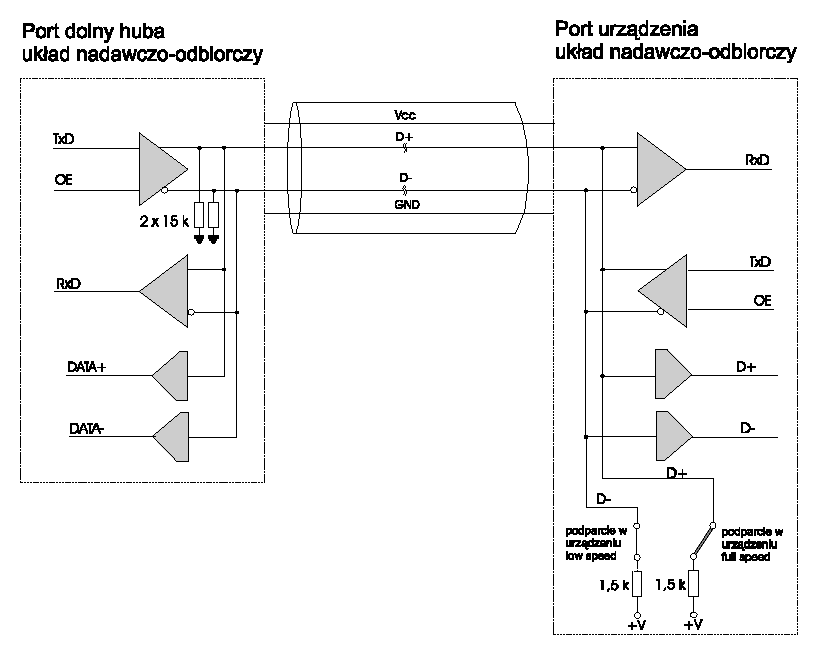
\includegraphics[width=10cm]{./wyklady/USB_7_1.pdf}
			\textbf{Stany magistrali USB}\\
			\begin{itemize}
				\item Logiczne „1” w obwodzie różnicowym (D+) - (D-) $>$ 200 mV
				\item Logiczne „0” w obwodzie różnicowym (D+) - (D-) $<$ -200 mV
				\item Plus 9 innych stanów
			\end{itemize}
			\textbf{Kodowanie bitów w systemie USB}\\
			W systemie USB przyjęto kodowanie NRZI (\emph{Non Return to Zero Inteverted}) ze wstawianiem bitu synchronizującego (tzw. \emph{bit stuffing}). Na początku każdego bitu o wartości logicznej zero następuje zmiana sygnału, natomiast po każdych 6 kolejnych bitach o wartości jeden wstawiany jest bit o wartości zero. Umożliwia to prawidłowe poznawanie bitów w sygnale odebranym bez potrzeby przesyłania sygnału zegarowego nadajnika. Bity wstawione są usuwane po rozpoznaniu stanu bitów w odebranym sygnale.\\\\
			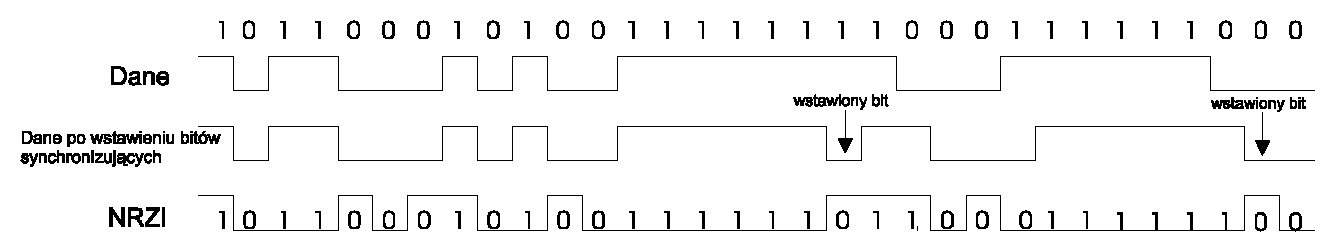
\includegraphics[width=15cm]{./wyklady/USB_9_1.pdf}
		\subsubsection{Srodowisko fizyczne}
			\textbf{Podstawowy kabel do podłączenia urządzenia USB}\\
			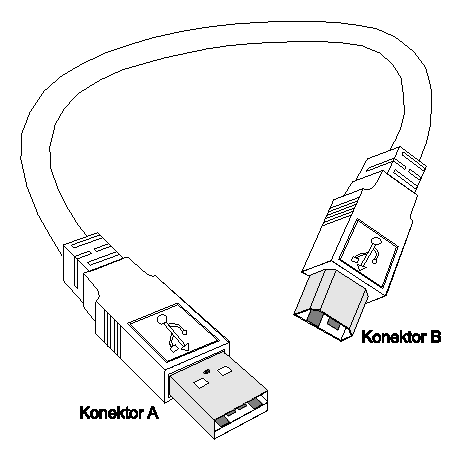
\includegraphics[width=6cm]{./wyklady/USB_10_1.pdf}\\
			W standardzie USB wyróżnia się dwa rodzaje złączy
			\begin{itemize}
				\item Konektor A – strona portu dolnego (hub), "od strony urządzenia"
				\item Konektor B – strona portu górnego (urządzenie), "od strony hosta"
			\end{itemize}
			Złącza USB posiadają 4 zaciski: po dwa dla magistrali danych i zasilania. W samym złączu kontakty zasilania są nieco wysunięte w przód przed kontakty danych, a więc po włożeniu najpierw jest podłączone zasilanie, a potem dane.
			\begin{table}[H]	%H z pakietu 'float' wymusza polozenie HERE  (bez tego zle ulozenie trsci)
				\begin{tabular}{|c|c|c|}
					\hline
					\textbf{Nr kontaktu}	& \textbf{Nazwa sygnału}	& \textbf{Kolor przewodu w kablu} \\ \hline
					1 						& Vcc						& Czerwony		\\ \hline
					2 						& +DATA						& Biały			\\ \hline
					3 						& -DATA						& Zielony		\\ \hline
					4 						& GND						& Czarny		\\ \hline
				\end{tabular}
			\end{table}
			\textbf{Rodzaje kabli}
			\begin{itemize}
				\item Kabel przeznaczony dla urządzeń „low speed”
				\begin{itemize}
					\item Nieekranowany
					\item Zawiera dwie, nieskręcane pary przewodów: dla danych (28 AWG) i zasilania (20-28 AWG)
				\end{itemize}
				\item Kabel przeznaczony dla urządzeń „full speed i high speed”
				\begin{itemize}
					\item Zawiera ekranowaną parę skręcaną (28 AWG) dla danych
					\item I nieekranowaną parę (20-28 AWG) dla zasilania
				\end{itemize}
				\item Czas propagacji sygnału w kablu: $<$ 30 ns przy przesyle z częstotliwością 1-16 MHz. Wymagany dla urządzeń małej i pełnej szybkości. Czas propagacji wpływa na długosc kabla:
				\begin{itemize}
					\item 5 m dla 6ns/m
					\item 3 m dla 10ns/m
				\end{itemize}
			\end{itemize}
		\subsubsection{Ramki i mikro ramki}
			W systemie USB dane są przekazywane:
			\begin{itemize}
				\item W ramkach o czasie trwania 1 $ms$ dla małej i pełnej szybkości transmisji.
				\item W mikroramkach o czasie trwania 125 $\mu s$ dla wysokiej szybkości transmisji.
			\end{itemize}
			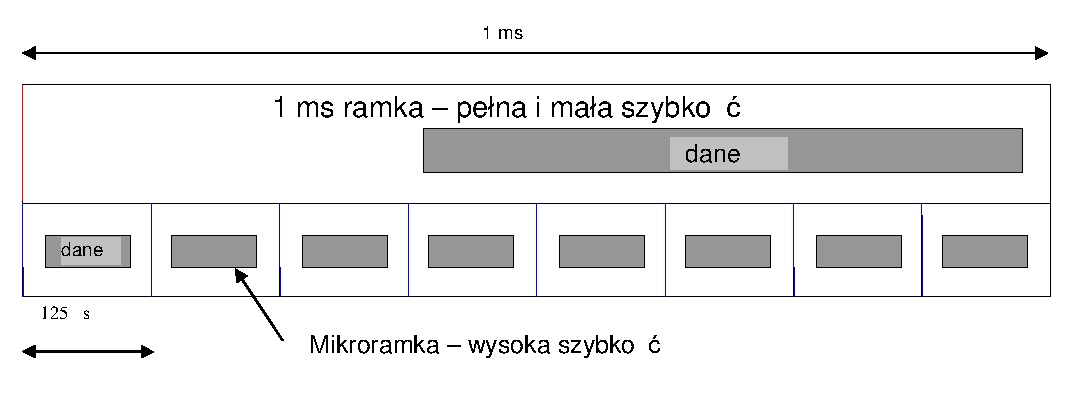
\includegraphics[width=10cm]{./wyklady/USB_11_1.pdf}\\
			\textbf{Ramka 1 ms}
			\begin{itemize}
				\item Czas pomiędzy dwoma kolejnymi pakietami SOF ($Start Of Frame$) nazywany jest ramką. Początek ramki wyznacza pakiet SOF zawierający 11 bitów danych i 5 bitów CRC. Dane w pakiecie SOF reprezentują kolejny numer ramki. Licznik ramek przepełnia się co 2048 ms.
				\item Pełna szybkość transmisji
				\begin{itemize}
					\item Maksymalny teoretyczny rozmiar ramki w bitach: 1 ms x 1/12 Mhz = 12000 bitów
					\item Powyższy rozmiar ramki w bajtach: 12000 : 8 = 1500.
					\item Pakiety kontrolne zajmują ok. 300 bajtów.
					\item Praktyczna górna granica liczby transmitowanych w ramce: 1200 bajtów.
				\end{itemize}
				\item Mała szybkość transmisji
				\begin{itemize}
					\item Max rozmiar ramki w bitach: 1 ms x 1/1,5 Mhz = 1500 bitów
					\item Max rozmiar ramki w bajtach: 1500 : 8 = 187
				\end{itemize}
			\end{itemize}
			\textbf{Mikroramka 125 $\mu s$}
			\begin{itemize}
				\item Czas pomiędzy dwoma kolejnymi pakietami SOF wysyłanymi przez high speed huba nazywa się mikroramką.
				\item Mikroramka trwa 125 $\mu s$
				\item Na 1 ramkę przypada 8 mikroramek
				\item Wysoka prędkość transmisji - szybkość transmisji w mikroramce wynosi 480 Mhz.
			\end{itemize}
			
		\subsubsection{Model komunikacyjny}
		Warstwowy model komunikacyjny przedstawiający odpowiadające sobie elementy sprzętowo-programowe po stronie hosta i urządzenia.
		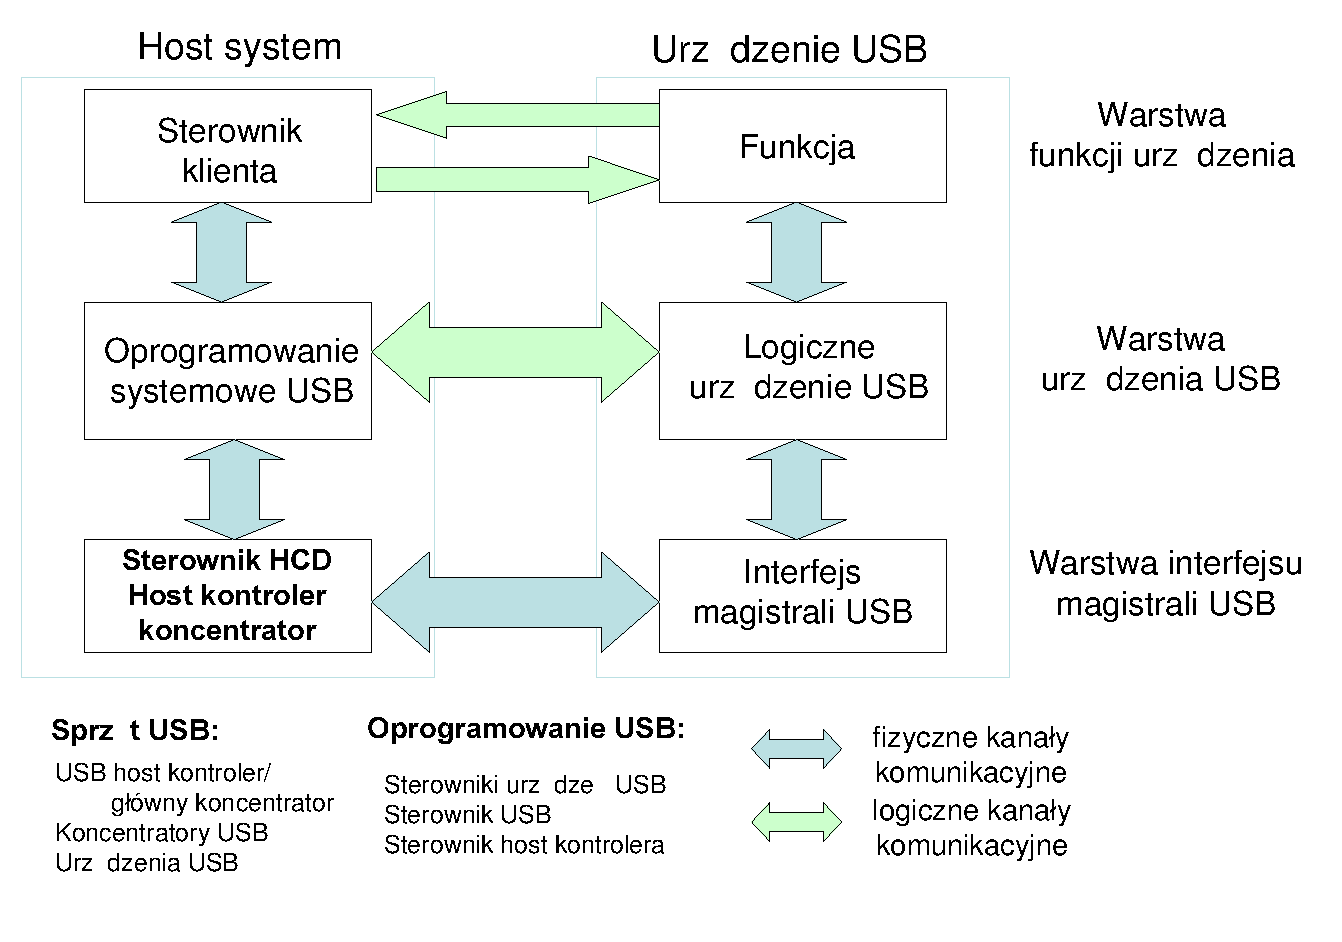
\includegraphics[width=10cm]{./wyklady/USB_12_1.pdf}\\\\
		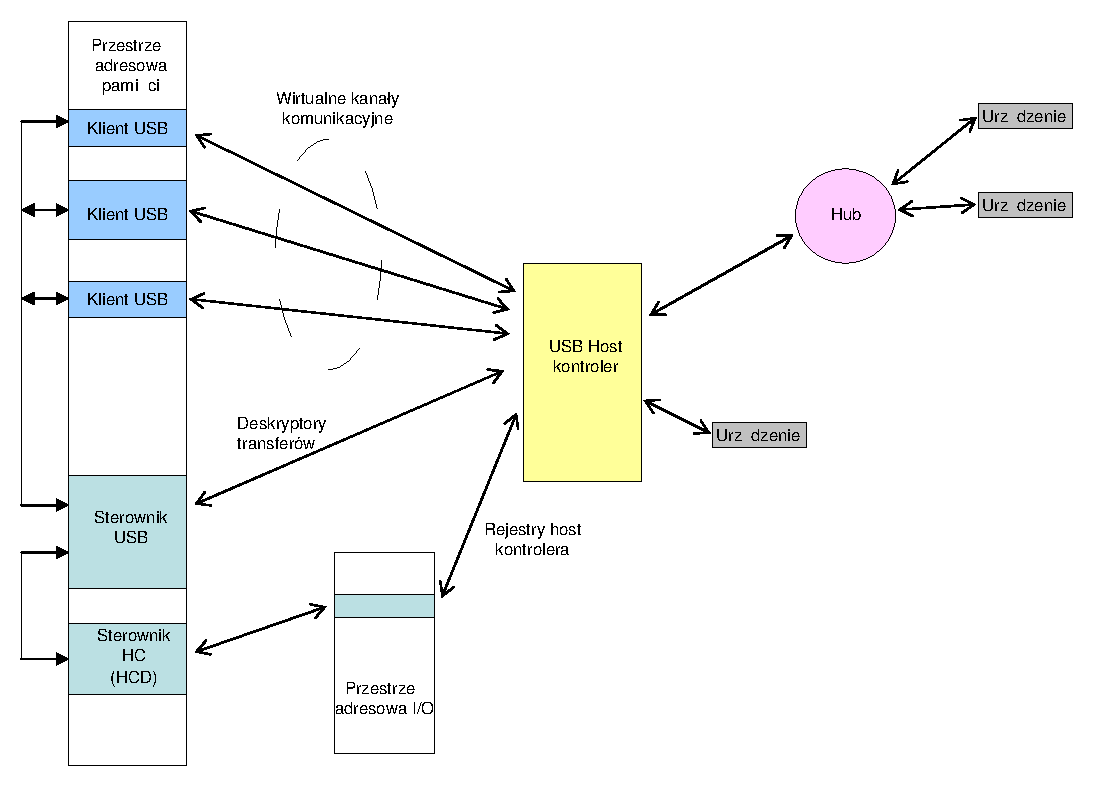
\includegraphics[width=10cm]{./wyklady/USB_13_1.pdf}\\
		\subsubsection{Transfery USB}
		Wyróżniono 4 typy transferów przeznaczone dla rożnych urządzeń z różnymi wymaganiami komunikacyjnymi. Każdy wymaga innego kanału komunikacyjnego (\emph{pipe}).
		\begin{itemize}
			\item \textbf{Masowy} (\emph{bulk transfer}) - time delivery accuracy + quality delivery accuracy ("jak najlepiej w miarę możliwości").\\
			Przeznaczony do komunikacji z urządzeniami, do których zapisuje się lub z których odczytuje duże ilości danych, jednak czas przekazywania danych oraz regularność ich dostarczania nie są krytyczne.\\
			Ważna jest kontrola przekazywanych danych, błędy transmisji muszą zostać wykryte i skorygowane poprzez żadanie ponownego przesłania błędnego bloku danych.\\
			Nie ma zagwarantowanego pasma, transmisja ta jest realizowana, jeżeli inne transfery nie wykorzystają przydzielonych im zasobów.\\
			Może być realizowany tylko z pełną lub wysoką szybkością.\\
			Wymagane jest, aby pakiet danych miał stałą wartość (\emph{MaxPacketSize}): 8, 16, 32 lub 64. Wszystkie kolejne pakiety danych muszą mieć tę stałą wartość z wyjątkiem ostatniego, który sygnalizuje koniec transferu.
			Przykłady: drukarka, skaner.
			\item \textbf{Przerwaniowy} (\emph{interrupt transfer}) - quality delivery accuracy.\\
			Do komunikacji z urządzeniami, do których zapisuje się lub z których odczytuje się niewielkie bloki danych, jednak trzeba robić to regularnie, w ustalonych odstępach czasowych.\\
			Parametry transferu zawarte są w deskryptorze pobieranym na etapie konfiguracji urządzenia.\\
			Ma zagwarantowane pasmo, może być wykorzystany do obsługi urządzeń low speed i full speed.\\
			Rozmiar pakietu danych zależy od wybranej szybkości: dla low speed jest to 8, dla full speed to maksymalnie 64. Wszystkie kolejne pakiety danych muszą mieć tę stałą wartość z wyjątkiem ostatniego, który sygnalizuje koniec transferu.\\
			Przykłady: mysz, klawiatura.
			\item \textbf{Izochroniczny} (\emph{isochronous transfer}) - time delivery accuracy.\\
			Przeznaczony do komunikacji z urządzeniami, do których zapisuje się lub z których odczytuje duże ilości danych, przy czym krytyczna jest regularność dostarczania danych.\\
			Nie jest ważna kontrola przekazywania danych, nie jest dopuszczalne ponowne wysłanie bloku danych.\\
			Dla komunikacji w pełnej lub wysokiej szybkości. Parametry transferu USB odczytuje z deskryptora urządzenia.\\
			Graniczna wartość parametru \emph{MaxPacketSize} to 1023 bajty na ramkę.\\
			Przykład: odtwarzanie muzyki w aparaturze audio.
			\item \textbf{Kontrolny} (\emph{control transfer}) - time delivery accuracy + quality delivery accuracy.\\
			Musi być obsługiwany przez każde urządzenie USB, ponieważ jest przeznaczony do jego konfiguracji i nadzoru. W ramce zarezerwowano stosowane pasmo dla realizacji transferów kontrolnych (10\% czasu trwania ramki).\\
			Obsługuje wszystkie 3 rodzaje prędkości transferu.\\
			Dzieli się na 3 etapy:
			\begin{itemize}
				\item Przekazanie rozkazu - 8-bitowe pole danych udostępnia informację o liczbie bajtów danych przesyłanych w etapie przekazani danych, o ile ten występuje.
				\item Przekazanie danych - pakiety danych mogą mieć rozmiar nie większy niż 64 bajty (parametr \emph{MaxPacketSize}).
				\item Przekazanie statusu.
			\end{itemize}
		\end{itemize}
		\textbf{Podział transferów}
		\begin{itemize}
			\item Transfery aperiodyczne: kontrolny i masowy
			\item Transfery periodyczne: przerwaniowy i izochroniczny
			\item Transfery strumieniowe (\emph{stream transfer}), przekazywanie danych bajt po bajcie: przerwaniowy, masowy i izochroniczny
			\item Transfery komunikatowe (\emph{message transfer}), struktura komunikatów i ich znaczenie określa standard: kontrolny
		\end{itemize}
		\subsubsection{Zarządzenie magistralą USB}
		Wszystkie transfery USB są inicjowane i kontrolowane przez hosta. Host usiłuje jednocześnie realizować transfery wielu urządzeń tak, aby jedno urządzenie nie blokowało dostępu.\\ 
		Niektóre transfery mają priorytety. Transferom izochronicznym i przerwaniowym nadano 90\% pasma, a kontrolnym 10\%. Oznacza to, że transfer masowy nie jest gwarantowany - jeżeli pozostałe 3 rodzaje zajmą maksymalny możliwy czas, to transfer masowy się nie odbędzie.\\
		W praktyce jednak zdarza się to rzadko i 3 transfery nie wykorzystują pełnego pasma, co pozwala kontrolerowi USB na przydzielenie niewykorzystanego miejsca transferom masowym.\\
		Kontroler dąży do jak najlepszego wykorzystania miejsca w ramce, w które może wstawić nawet wiele transakcji danego transferu masowego.\\
		Działanie kontrolera oparte jest na zasadzie "usilnych starań" (\emph{best efforts}), aby jak najsprawniej (w jak najkrótszym czasie) zrealizować wszystkie żądane transfery. Jednak jeżeli w ramce 1 ms brakuje miejsca na transferu masowego to musi on czekać.
		\subsubsection{Stany urządzenia USB}
		Zanim urządzenie USB zostanie skonfigurowane i udostępnione aplikacjom musi przejść przez kilka stanów przestawionych na rysunku\\
		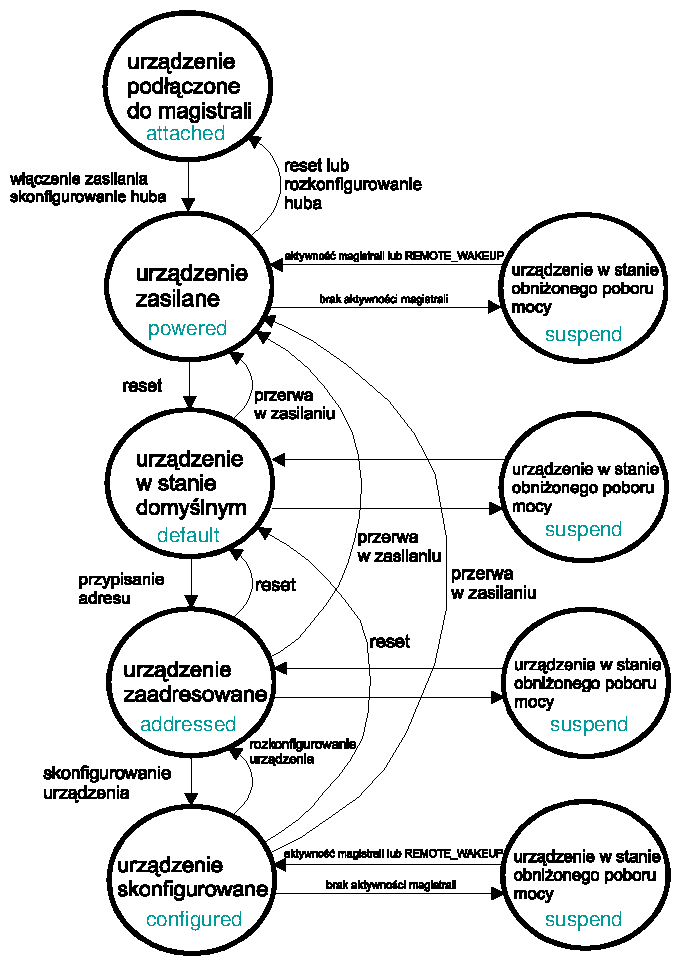
\includegraphics[width=10cm]{./wyklady/USB_16_1.pdf}
		\subsubsection{Hub w systemie USB}
		Huby to urządzenia pośredniczące w komunikacji z urządzeniami końcowymi.
		\begin{itemize}
			\item Zwiększają liczbę portów dostępnych dla urządzeń oraz możliwe jest ich kaskadowe łączenie.
			\item Port huba od strony hosta nazywa się górnym (\emph{uper stream port}), natomiast porty od strony urządzeń dolnym (\emph{down stream port}).
			\item Hub przeważnie posiada 4 porty dolne, rzadko kiedy inną liczbę jak np. 7.
			\item Hub nie tylko przekazuje dane, ale pośredniczy również w dystrybucji zasilania do urządzeń.
			\item Huby zgodne ze standardem 1.x są zdolne do komunikacji z małą lub pełną szybkością. Obowiązuje zasada, że do urządzeń low speed nie wolno kierować ruchu full speed. Hub potrafi wykryć jakie urządzenie jest podłączone do danego portu dolnego i wie, kiedy należy go zablokować.
			\item Transfery low speed są poprzedzone specjalną preambułą, których zadaniem jest odblokowanie portów dolnych do których podłączone są urządzenia low speed.
		\end{itemize}
		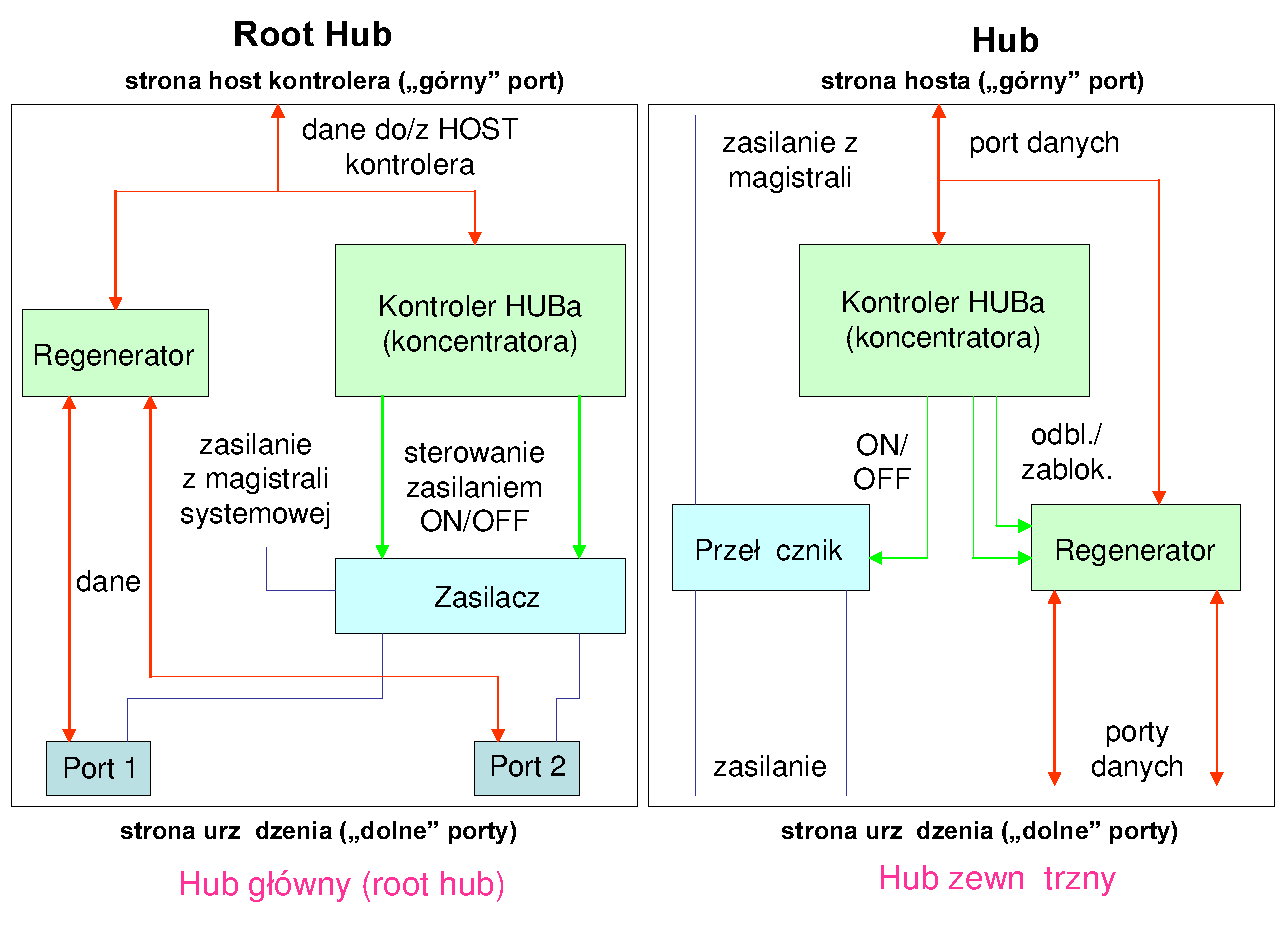
\includegraphics[width=10cm]{./wyklady/USB_17_1.pdf}
	
\subsection{Protokół komunikacyjny}
	Transakcje USB zbudowane sa z pakietów, przy czym typowa transakcja zawiera:
	\begin{itemize}
		\item Pakiet tokena (\emph{token packet}) - jest elementem kontrolnym transakcji i informuje o jej rodzaju: kontrolna lub przeznaczona do zapisywania danych.
		\item Pakiet danych (\emph{data packet}) - pole przeznaczone dla danych zapisywanych do urządzenia lub odczytywanych z urządzenia.
		\item Pakiet potwierdzenia (\emph{handshake packet}) - informuje jednostkę nadającą o odebraniu danych lub instrukcji sterującej przez odbiorcę.
	\end{itemize}
	\subsubsection{Właściwości}
	\begin{itemize}
		\item Komunikacja z urządzeniami USB za pomocą ramek o długości maksymalnie 1 ms.\\
		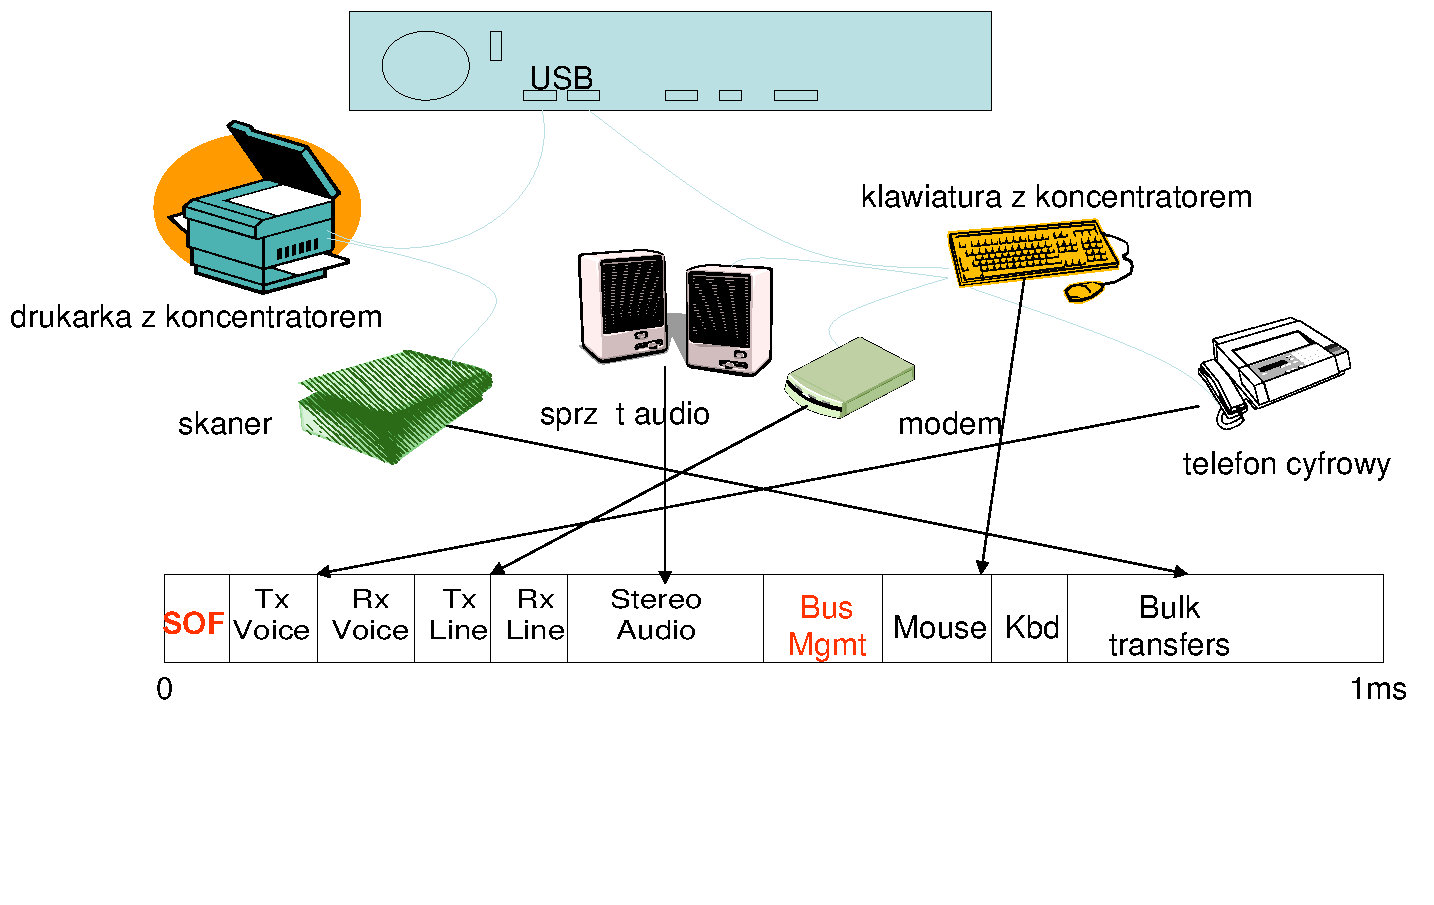
\includegraphics[width=10cm]{./wyklady/USB_18_1.pdf}
		\item Pakietowa struktura komunikatów\\
		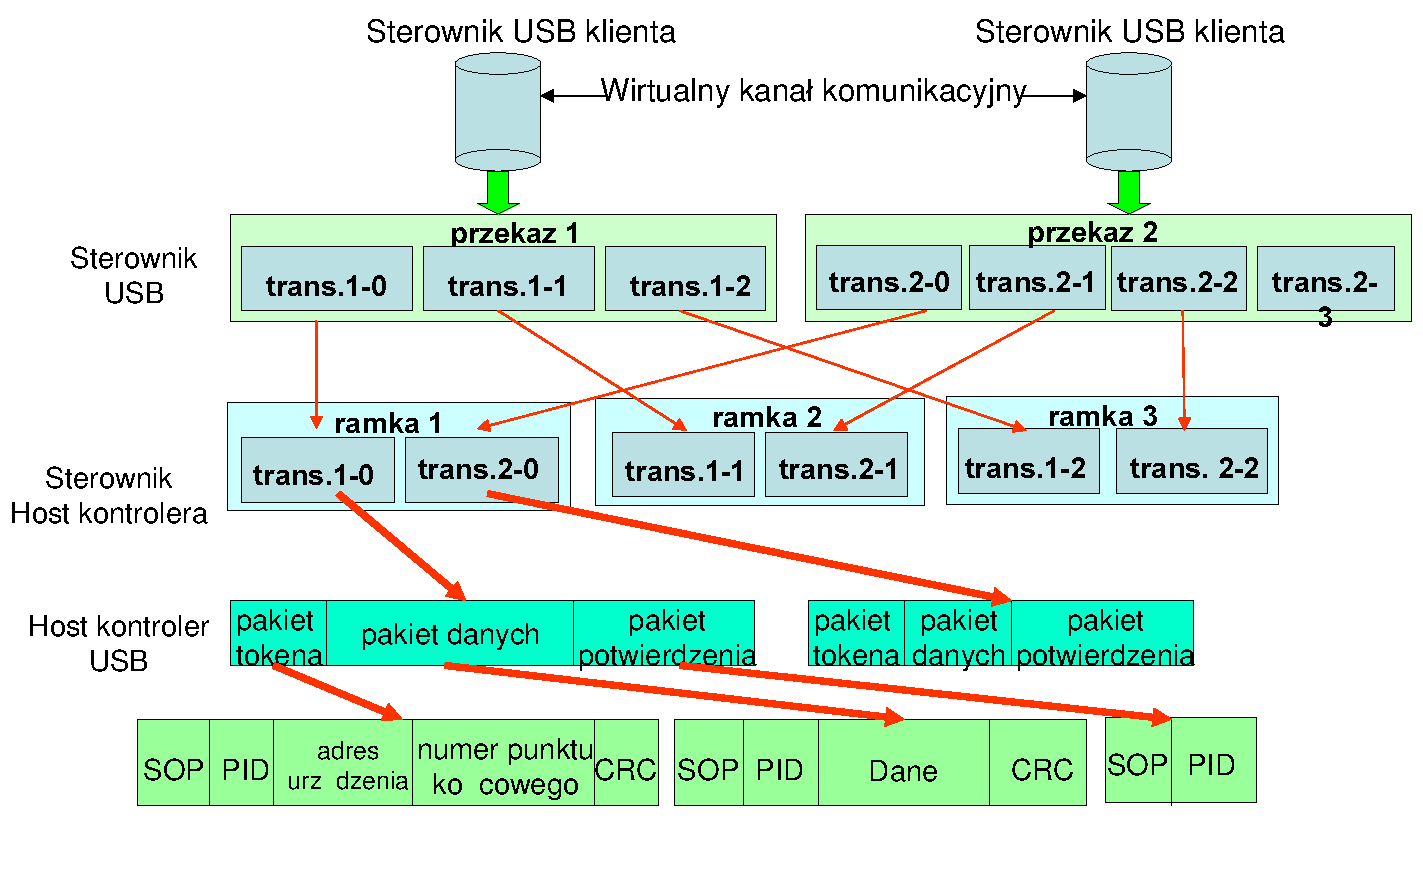
\includegraphics[width=10cm]{./wyklady/USB_19_1.pdf}\\
		Struktura bloków komunikacyjnych w USB
	\end{itemize}
	\subsubsection{Format i typy pakietów USB}
	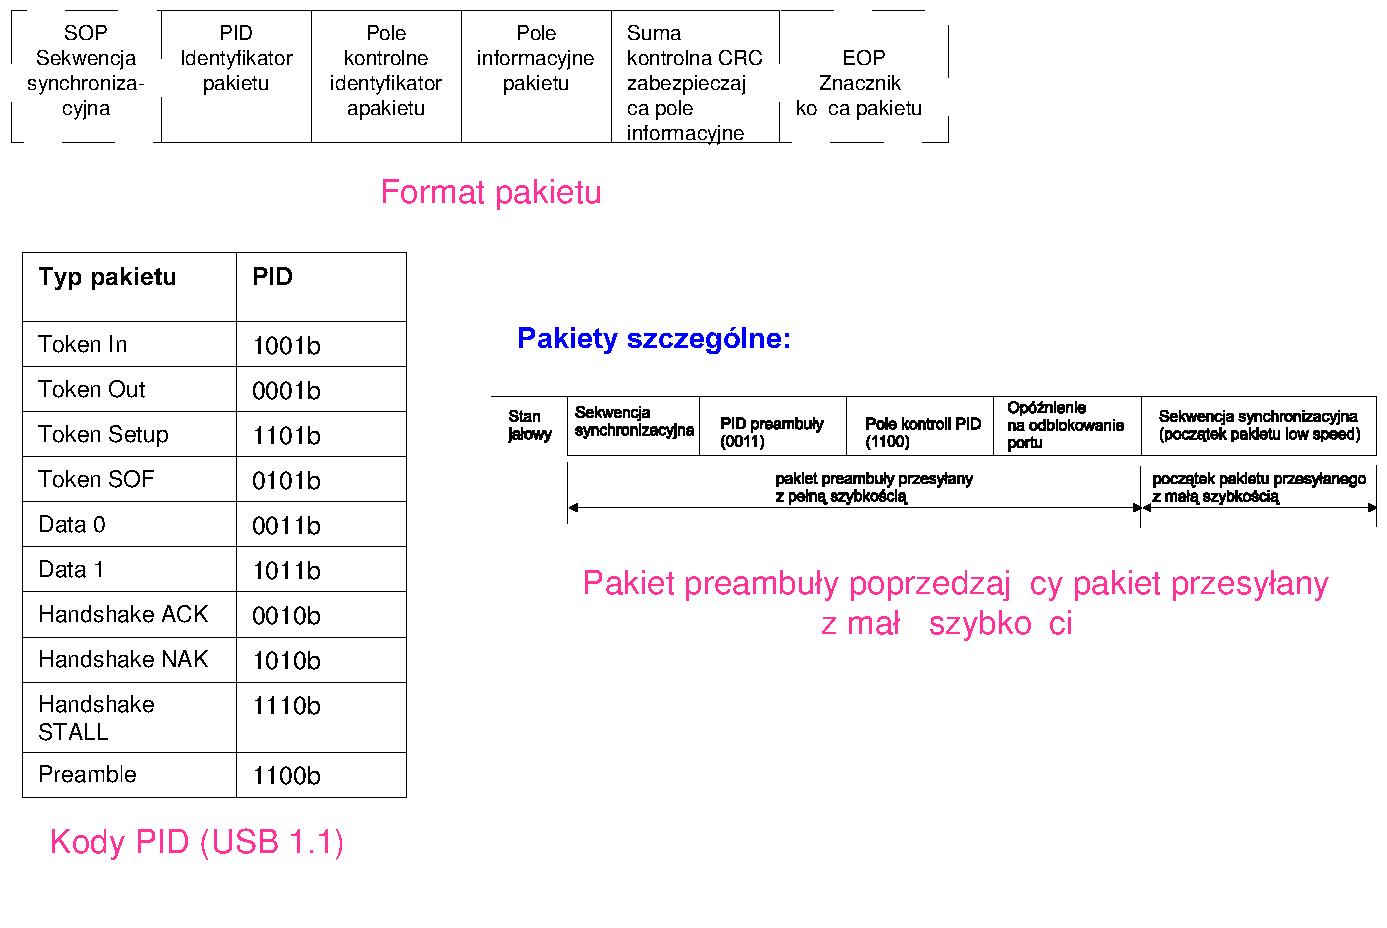
\includegraphics[width=10cm]{./wyklady/USB_20_1.pdf}
	\subsubsection{Reakcja na błędy}
	Wykrywanie błędów i kontrola transmisji\\
	\begin{itemize}
		\item Kontrola poprawności pakietów (zabezpieczenie pola PID sumą CRC)
		\begin{itemize}
			\item W przypadku pakietu Token - 5-bitowa suma
			\item W przypadku pakietu Data - 16-bitowa suma
		\end{itemize}
		Wykrycie błędu powoduje odrzucenie pakietu.
		\item Reakcja na fałszywy znacznik końca pakietu (\emph{false EOP})
		\item Ograniczenie czasowe oczekiwania na odpowiedź
		\item Przełączanie kolejnych pakietów danych (mechanizm \emph{data toogle})
		\item Wykrywanie transakcji występujących po zakończeniu ramki (tzw. „paplanie” – \emph{babble})
		\item Wykrywanie braku aktywności magistrali (LOA – \emph{Loss Of Activity})
	\end{itemize}
	Transfer kontrolny, przerwaniowy i masowy wysyłają pakiet ponownie, jeżeli jest on błędu, nie informując odbiorcy o tym. Transfer izochroniczny nie.
	\subsubsection{Czas obiegu (\emph{round trip delay})}
	Ograniczenie czasowe oczekiwania na odpowiedź. Jest to podstawowy mechanizm informowania nadawcy o niepoprawnym przekazaniu pakietu. Ograniczenie czasowe nie może być mniejsze od 16*(\emph{czas trwania bitu}), ani większe od 18*(\emph{czas trwania bitu}).\\
	Poniżej połączenie urządzenia z hostem przez 5 hubów – najgorszy przypadek pod względem czasowym.\\
	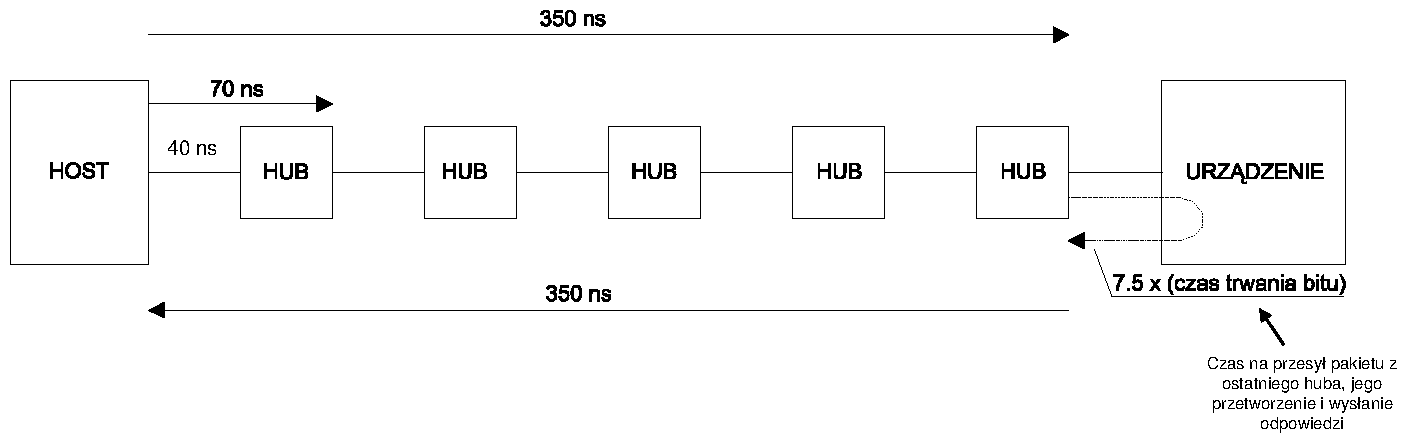
\includegraphics[width=10cm]{./wyklady/USB_23_1.pdf}\\
	Jest on podstawa do rozważań na temat ograniczeń tego czasu.
	\begin{itemize}
		\item Round trip delay: 2 x 350 ns = 700 ns
		\item Czas trwania 1 bitu dla full speed: 1/12 MHz = 83 ns
		\item Round trip delay w bitach dla full speed: 700 ns/83 ns = 8,5 bitu
		\item Timeout oczekiwania na odpowiedź: 7,5 bitu (specyfikacja) + 8,5 bitu = 16 bitów
	\end{itemize}
	
\subsection{Deskryptory w urządzeniach USB}
	W każdym urządzeniu USB znajduje się pełna informacja o sposobie komunikacji z urządzaniem, udostępniana podczas procesu enumeracji.\\
	Informacja ta jest przechowywana w deskryptorach - tablicach o ściśle określonej strukturze.
	\subsubsection{Hierarchiczna struktura deskryptorów w urządzeniu USB}
	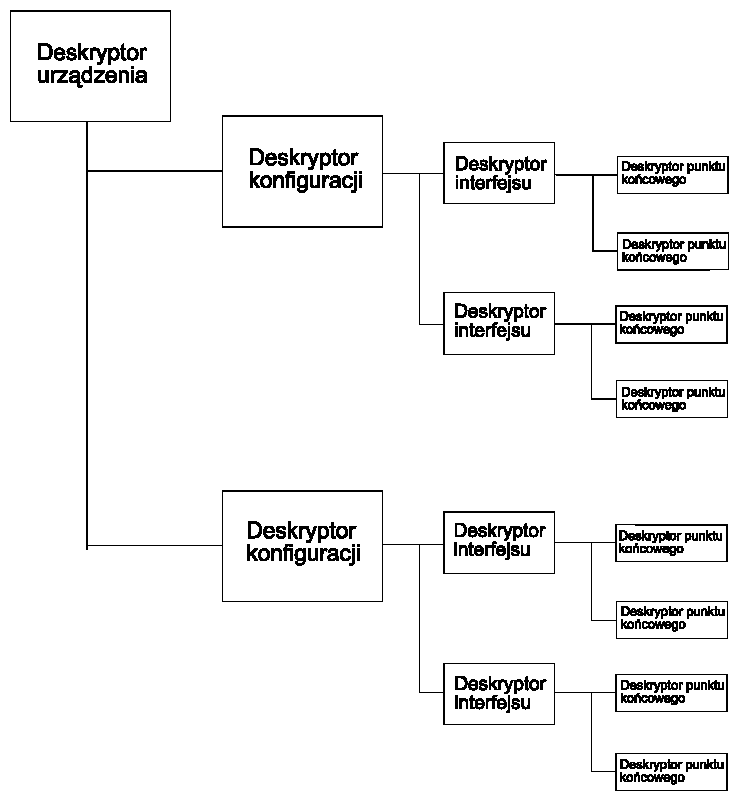
\includegraphics[width=10cm]{./wyklady/USB_24_1.pdf}
	\subsubsection{Rodzaje deskryptorów}
	\begin{itemize}
		\item Deskryptor urządzenia - m.in. liczba konfiguracji dostępnych w urządzeniu.
		\item Deskryptor konfiguracji - opisuje każdą konfigurację z osobna. Zawiera informację o liczbie interfejsów przypisanych danej konfiguracji.
		\item Deskryptor interfejsu - posiada go każdy interfejs, który określa m.in. liczbę punktów końcowych z nim związanych.
		\item Deskryptor punktu końcowego - charakteryzuje każdy punkt końcowy.
		\item Deskryptor łańcuchowy - zawiera kod określający język tekstu lub sam właściwy tekst.
	\end{itemize}
	
\subsection{Wykrywanie i konfiguracja urządzeń}
	Cechą USB jest automatyczne wykrywanie urządzeń po włączeniu zasilania w systemie lub włączeniu urządzenia do systemu. Procedura enumeracji zajmuje się rozpoznaniem urządzenia, sprawdzeniem czy komunikacja jest możliwa, przydzieleniem adresu, konfiguracją i instalacją sterownika.
	\subsubsection{Procedura enumeracji urządzenia}
	\begin{enumerate}
		\item Automatyczne wykrycie urządzenia - powoduje ustawienie bitu w rejestrze statusu huba, który odpowiada temu portowi.
		\item Odblokowanie portu i generacja RESETU - przejście do stanu domyślnego.
		\item Odczyt deskryptora urządzenia - skierowanie stosownego rozkazu do punktu końcowego 0 o adresie 0. Jest tylko jedno takie urządzenie w systemie - te, które właśnie podlega procesowi enumeracji.
		\item Przypisanie adresu - unikalny adres dla urządzenia
		\item Odczyt pozostałych deskryptorów - jeżeli istnieją
		\item Konfiguracja urządzenia
		\item Instalacja sterownika klienta
		\item Urządzenie jest dostępne dla aplikacji
	\end{enumerate}
	
\subsection{Kontrola urządzenia – transfer kontrolny}
	Transfer kontrolny służy do sterowania urządzeniem. Urządzenie USB otwiera kontrolny kanał komunikacyjny pomiędzy hostem, a punktem końcowym 0 w urządzeniu.
	\subsubsection{Etapy transferu kontrolnego}
	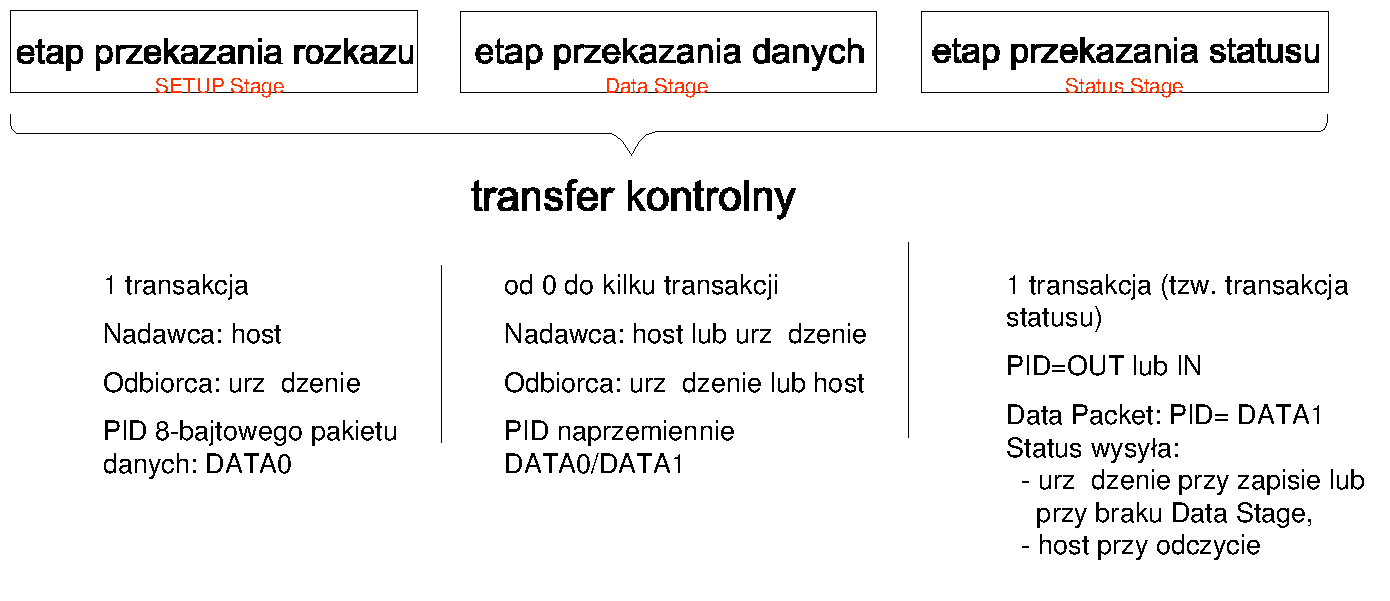
\includegraphics[width=10cm]{./wyklady/USB_31_1.pdf}
	\begin{enumerate}
		\item Przekazanie rozkazu (\emph{Setup Stage}) - jak w każdym pakiecie Token, następne pola zawierają adres urządzenia oraz punktu końcowego. Kolejnym elementem jest 8-bajtowy pakiet danych typu Data 0, który specyfikuje rozkaz.
		\item Przekazanie danych (\emph{Data Stage}) - jeżeli 8 bajtów z powyższego nie wystarcza, wtedy jest ten etap. Liczbę bajtów do przekazania określa słowo Length w polu transakcji Setup. Jeżeli ta liczba nie przekracza wartości \emph{MaxPacketSize} to do przekazania danych wystarcza jedno transakcja, w przeciwnym razie odpowiednio dzieli się na więcej transakcji (sufit(Length \ MPC)).
		\item Przekazanie statusu (\emph{Status Stage}) - potwierdzenie wykonania transferu lub poinformowanie o niepowodzeniu w realizacji. Normalnie występuje do zakończeniu transakcji, ale host może rozpocząć ją wcześniej, w Data Stage (wtedy DS jest przerywane).
	\end{enumerate}
	
\subsection{Hub USB}
	\subsubsection{Co to jest?}
	Standard USB definiuje oddzielną klasę urządzeń: klasa HUB. Jest to tak ważna część tego systemu, że została zdefiniowana w standardzie USB, a nie we własnej oddzielnej specyfikacji.\\
	Typowy hub posiada jeden deskryptor.
	\subsubsection{HUB zasilany z magistrali}
	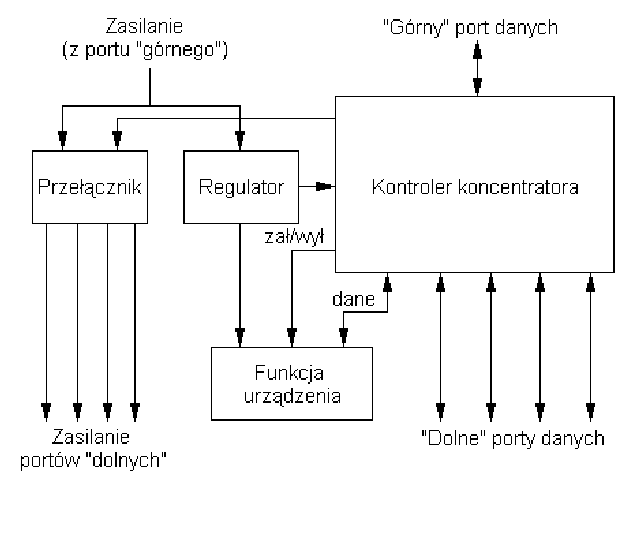
\includegraphics[width=10cm]{./wyklady/USB_34_1.pdf}
	\subsubsection{Proces konfiguracyjny huba}
	\begin{itemize}
		\item Odczyt standardowych deskryptorów urządzenia
		\item Przypisanie hubowi adresu
		\item Załączenie zasilania na porty, co jest niezbędne do detekcji podłączonych do portu urządzeń
		\item Odczyt punktu końcowego, "zmiany w hubie", w celu wykrycia urządzeń podłączonych do portów
		\item Odblokowanie portu w celu umożliwienia dostępu do urządzenia
	\end{itemize}
	\subsubsection{Punkt końcowy huba "zmiany w hubie"}
	\begin{itemize}
		\item Cyklicznie odczytywany, umożliwia monitorowanie zmian na portach dolnych huba, co z kolei umożliwia wykrywanie dołączania i usuwania urządzeń.
		\item Odpytywanie odbywa się przez wykorzystanie kanału przerwaniowego.
		\item \emph{Hub change point}: informuje o wystąpieniu:
		\begin{itemize}
			\item Zmiany w zasilaniu lub nadmiernym obciążeniu prądowym huba
			\item Zmiany na jednym lub kilku portach dolnych spowodowanej dołączeniem lub odłączeniem urządzenia.
		\end{itemize}
		\item Odczyt \emph{Hub change point} zwraca bajt statusowy huba. Jeżeli hub posiada więcej niż 7 portów dolnych - zwracane są dwa bajty.
		\item Jeżeli wszystkie bity w punkcie końcowym sa ustawione na 0 (brak zmian), hub nie odsyła bajtu statusowego.
		\item Nie mylić z punktem końcowym 0 przez który wykonywana jest konfiguracja i kontrola.
	\end{itemize}
	\subsubsection{Działanie}
	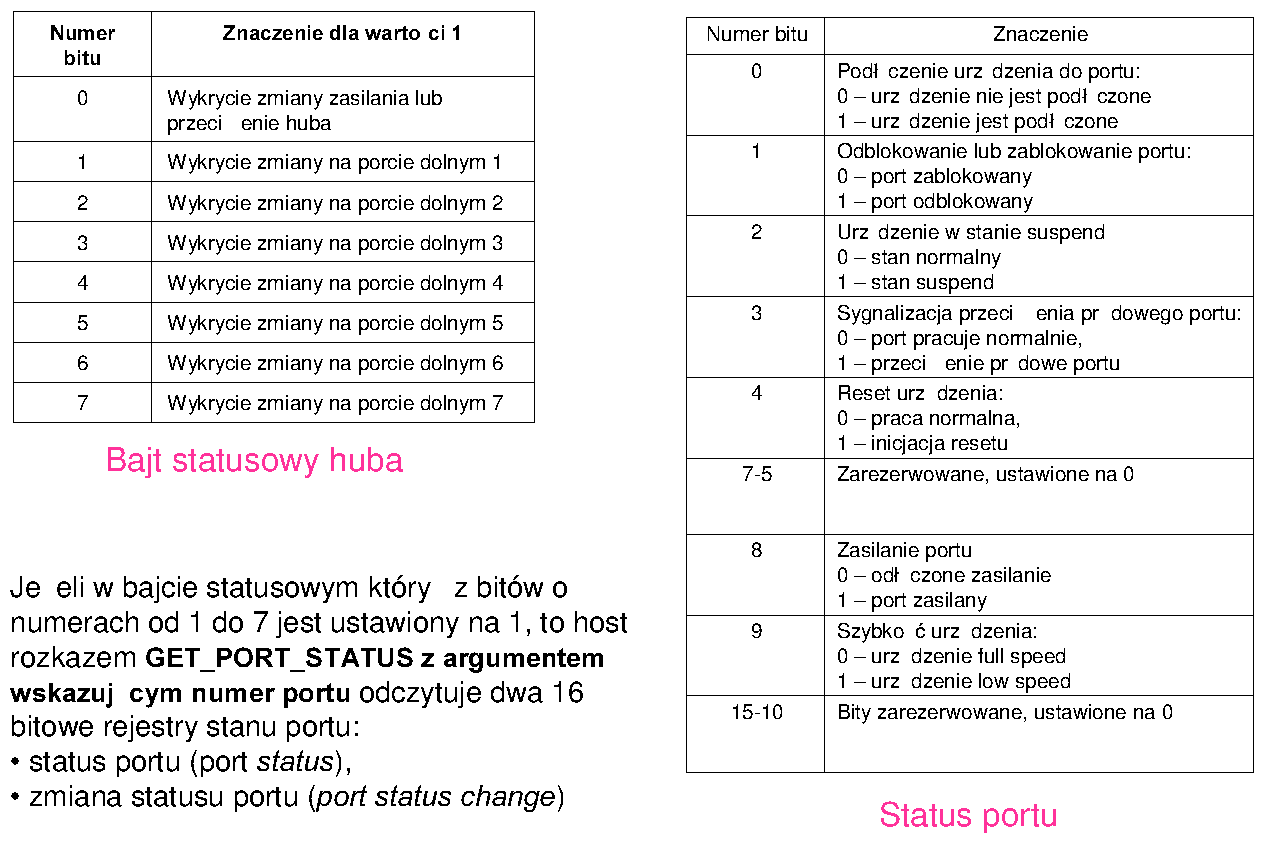
\includegraphics[width=8cm]{./wyklady/USB_35_1.pdf}
	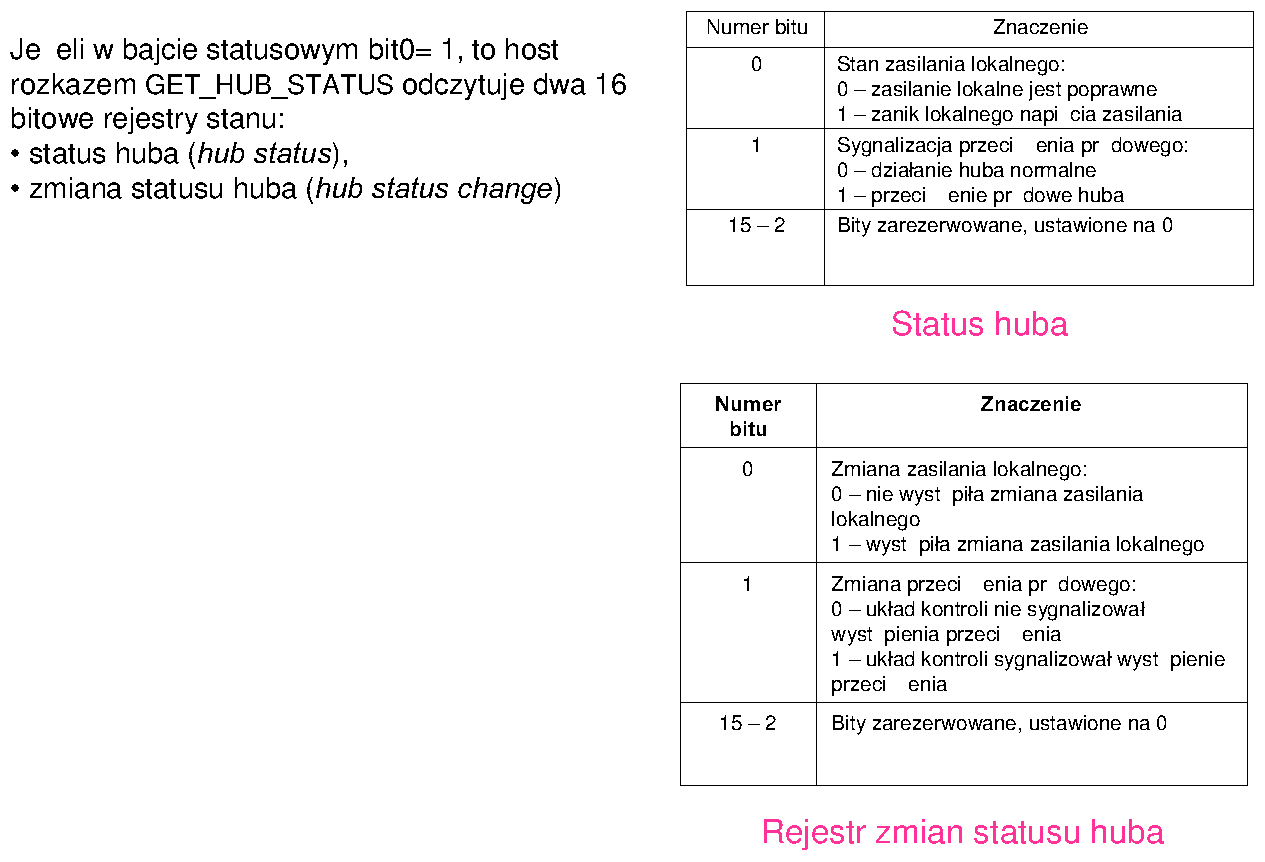
\includegraphics[width=8cm]{./wyklady/USB_36_1.pdf}
	
\subsection{Zasilanie urządzeń w systemie USB}
	USB jest również systemem dystrybucji i zarządzania zasilaniem urządzeń.
	\subsubsection{Możliwe zasilania urządzeń USB}
	\begin{itemize}
		\item Urządzenie zasilane z magistrali
		\item Urządzenie zasilane z własnego źródła
		\item Urządzenie zasilane częściowo z magistrali i własnego źródła
	\end{itemize}
	\subsubsection{Zasilanie hubów i pozostałych urządzeń}
		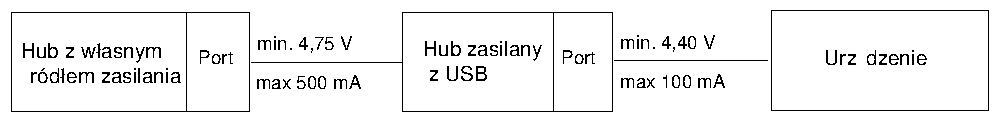
\includegraphics[width=11cm]{./wyklady/USB_38_1.pdf}\\
		Dopuszczalne spadki napięcia zasilania.
	\subsubsection{Urządzenie zasilane z magistrali}
		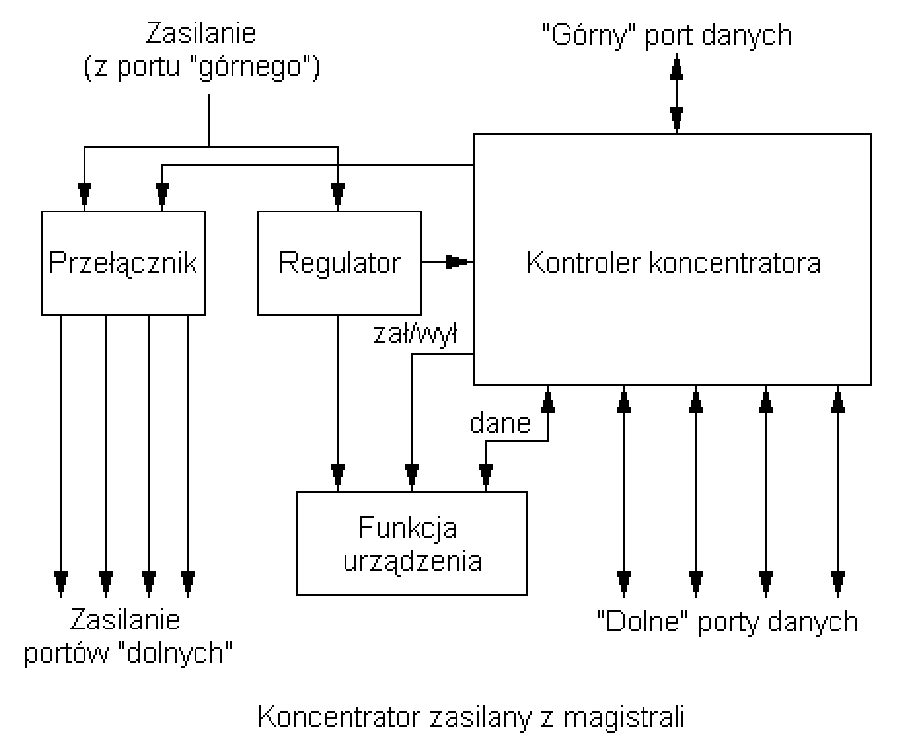
\includegraphics[width=7cm]{./wyklady/USB_39_1.pdf}\\
		Dla portu zasilanego z magistrali USB i podłączonego do portu o obciążalności 500 mA, 100 mA jest zarezerwowane na zasilanie jego układu. Oznacza to, że 400 mA pozostaje dla jego portów dolnych. Ponieważ każdy port musi mieć zapewnione minimum 100 mA, taki hub może mieć nie więcej niż 4 porty dolne (stąd pewnie przyjęty standard).
	\subsubsection{Zarządzanie zasilaniem}
	\begin{itemize}
		\item Wprowadzenie w \textbf{stan zawieszenia} pracy systemu – \emph{suspend}. Pozostając w zawieszenie urządzenie zachowuje swoją konfigurację, co pozwala jego wznowienie (\emph{resume}) do normalnego działania.
		\begin{itemize}
			\item \textbf{Globalne} (\emph{global suspend}) - rozkaz SetPortFeature (PORT\_SUSPEND) adresowany do huba głównego, zawiesza cały system
			\item \textbf{Częściowe} (\emph{selective suspend}) - rozkaz SetPortFeature (PORT\_SUSPEND) adresowany do huba zewnętrznego, w którym wybrany port (lub część systemu) ma zostać zawieszony.
			\item Zawieszone porty nie propaguj ruchu „w dół” oraz nie przekazują „w górę” żadnych sygnałów od urządzeń do nich podłączonych.
			\item Urządzenia w stanie zawieszenia zachowują swój stan, co umożliwia wznowienie ich pracy bez ponownej konfiguracji.
			\item Hub w stanie zawieszenia dodatkowo blokuje wszystkie nadajniki, zatrzymuje wewnętrzne zegary i zachowuje stan wszystkich portów dolnych.
			\item Urządzenie w stanie zawieszenie pobiera prąd $< 500 [\mu A]$
			\item Urządzenie automatycznie przechodzi do stanu \emph{SUSPEND} po wykryciu braku aktywności magistrali przez 3 $ms$. (USB wysyła ramki co 1 ms)
			\begin{itemize}
				\item Urządzenia pełnej szybkości wykorzystują pakiety SOF
				\item Urządzenia małej szybkości wykorzystują generację przejścia ze stanu jałowego do stanu K w odstępach czasu nie większych niż 3 ms.
			\end{itemize}
		\end{itemize}
		\item \textbf{Wznowienie} pracy systemu - \emph{resume}
		\begin{itemize}
			\item Globalne
			\item Wake-up
			\item Wznowienie pracy urządzenia można nastąpić
			\begin{itemize}
				\item Z inicjatywy kontrolera, jako wznowienie po zawieszeniu globalnym lub częściowym\\
				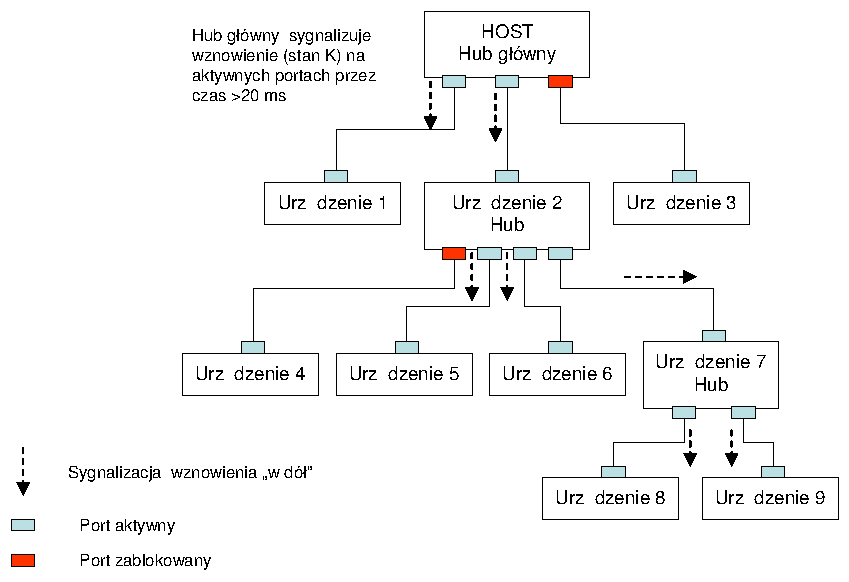
\includegraphics[width=7cm]{./wyklady/USB_43_1.pdf}
				\item Z inicjatywy urządzenia, po wystąpieniu zdarzenia wymagającego obsługi („budzenie” - \emph{Wakeup})\\
				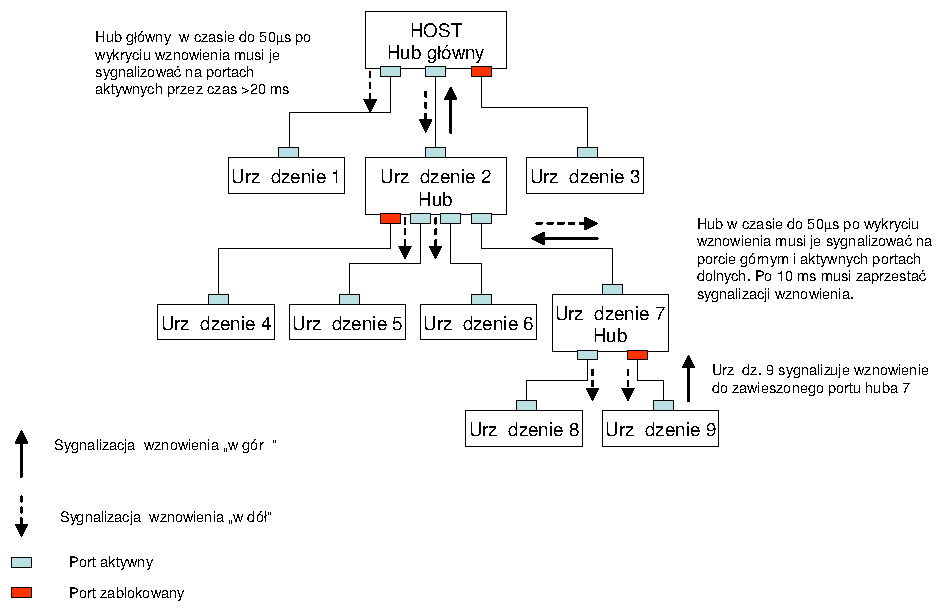
\includegraphics[width=7cm]{./wyklady/USB_44_1.pdf}
			\end{itemize}
			\item Wznowienie po zawieszeniu globalnym - rozpoczyna hub główny wykonując rozkaz wznowienia pracy systemu. Oznacza gotowość wszystkich hubów i urządzeń do wykonywania transakcji.
			\item Wznowienie po częściowym zawieszeniu - może wykonać:
			\begin{itemize}
				\item Host rozkazem \emph{ClearPortFeature} (PORT SUSPEND) adresowanym do huba w którym znajduje się zawieszony port.
				\item Urządzenie podłączone do zawieszonego portu poprzez \emph{Wakeup}
			\end{itemize}
		\end{itemize}
	\end{itemize}
	
\subsection{Rozwiązania host kontrolerów}
	\subsubsection{Co to jest?}
	Host kontrolera (\emph{Host Controller Driver}) przetwarza poszczególne IRP na transakcje, tworzy listę transakcji  w ramach ramki, przygotowuje scenariusz wykonania każdej transakcji i kontroluje jej wykonanie.
	\subsubsection{Rozwiązania}
	Opracowano dwa rozwiązania host kontrolera:
	\begin{itemize}
		\item Uniwersalny host kontroler - \emph{Universal Host Controler} (Intel)
		\item Otwarty host kontroler – \emph{Open Host Controler} (Compaq, Microsoft, National Semiconductor)
	\end{itemize}
	Są do siebie bardzo podobne, różnią się tylko sposobem obsługi oraz współpracą z hubem głównym.
	\subsubsection{Uniwersalny host kontroler (UHC)}
	\textbf{Zasada działania kontrolera UHC}\\
	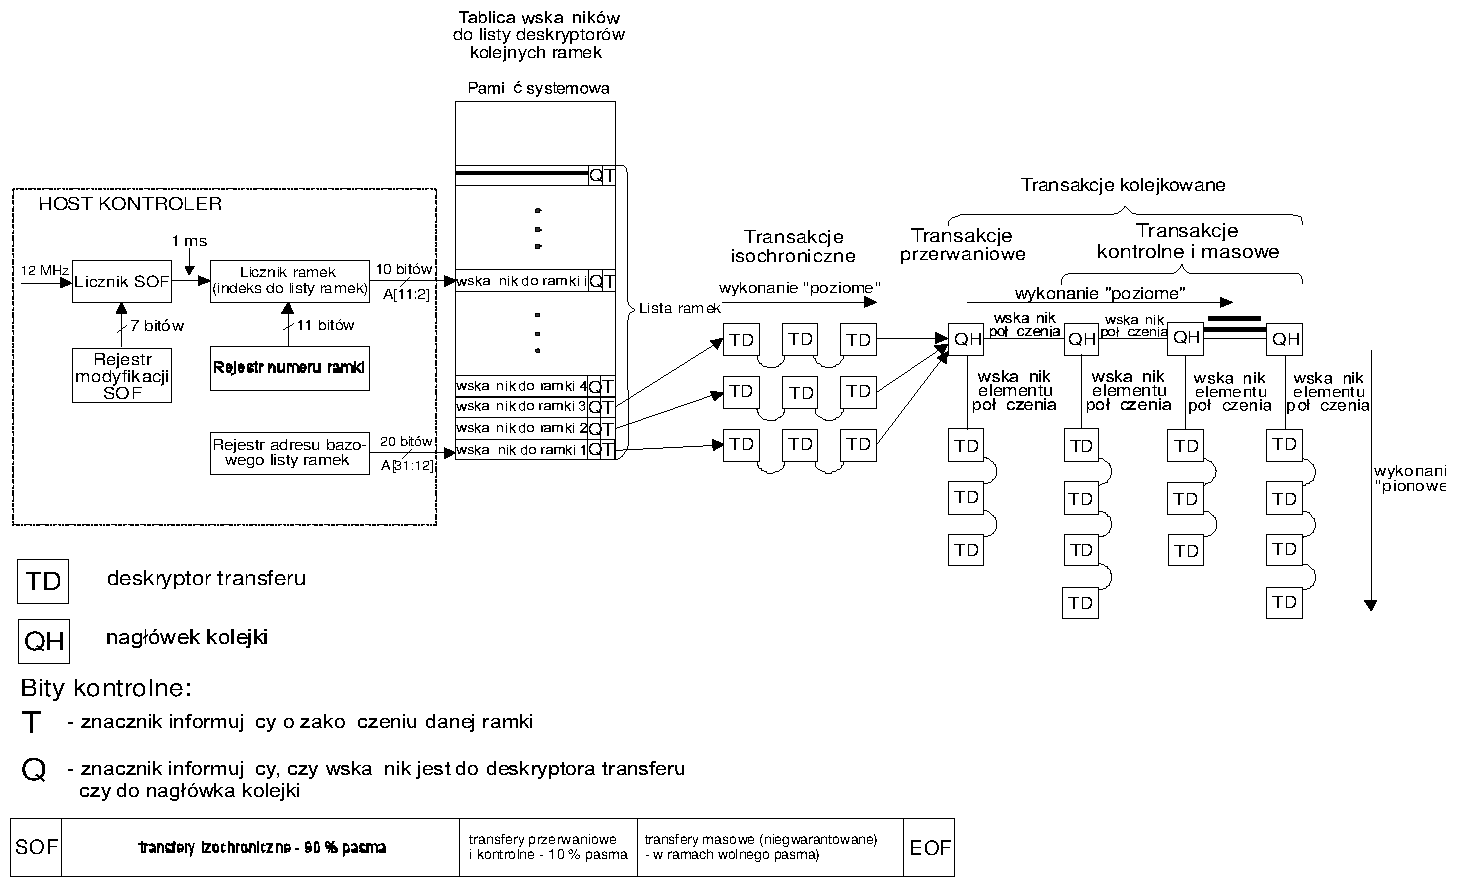
\includegraphics[width=7cm]{./wyklady/USB_46_1.pdf}\\\\
	\textbf{Ogólna postać deskryptora transferu (TD)}\\
	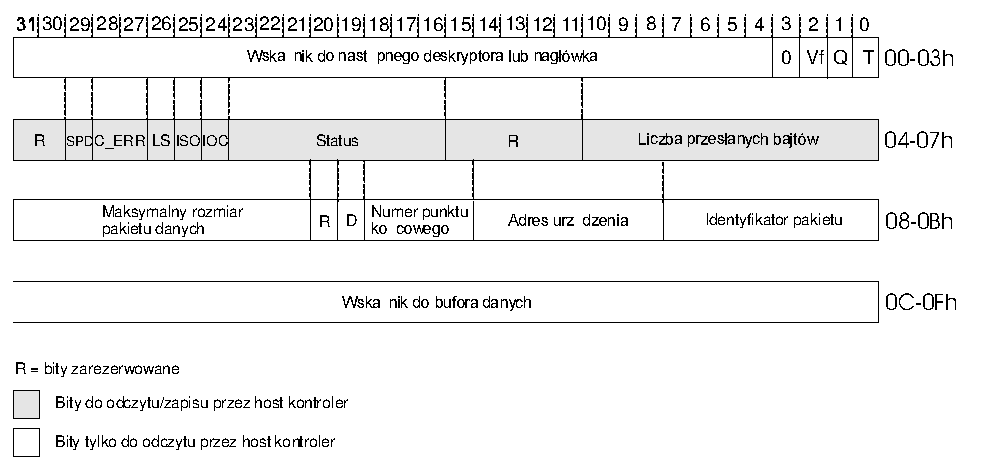
\includegraphics[width=7cm]{./wyklady/USB_47_1.pdf}\\\\
	\textbf{Ogólna postać nagłówka kolejki (QH)}\\
	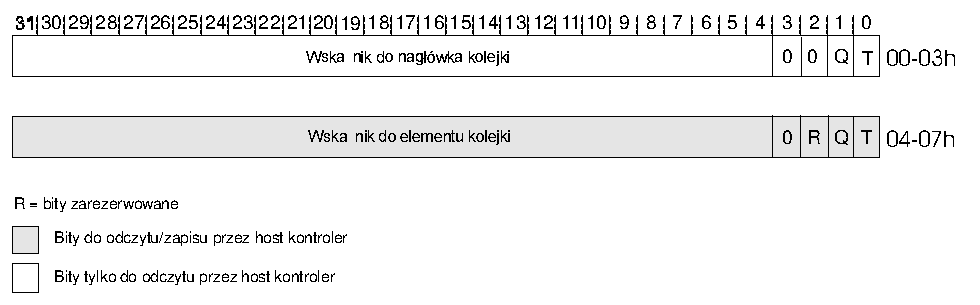
\includegraphics[width=7cm]{./wyklady/USB_48_1.pdf}
	\subsubsection{Otwarty host kontroler (OHC)}
	\textbf{Zasada działania kontrolera OHC}\\
	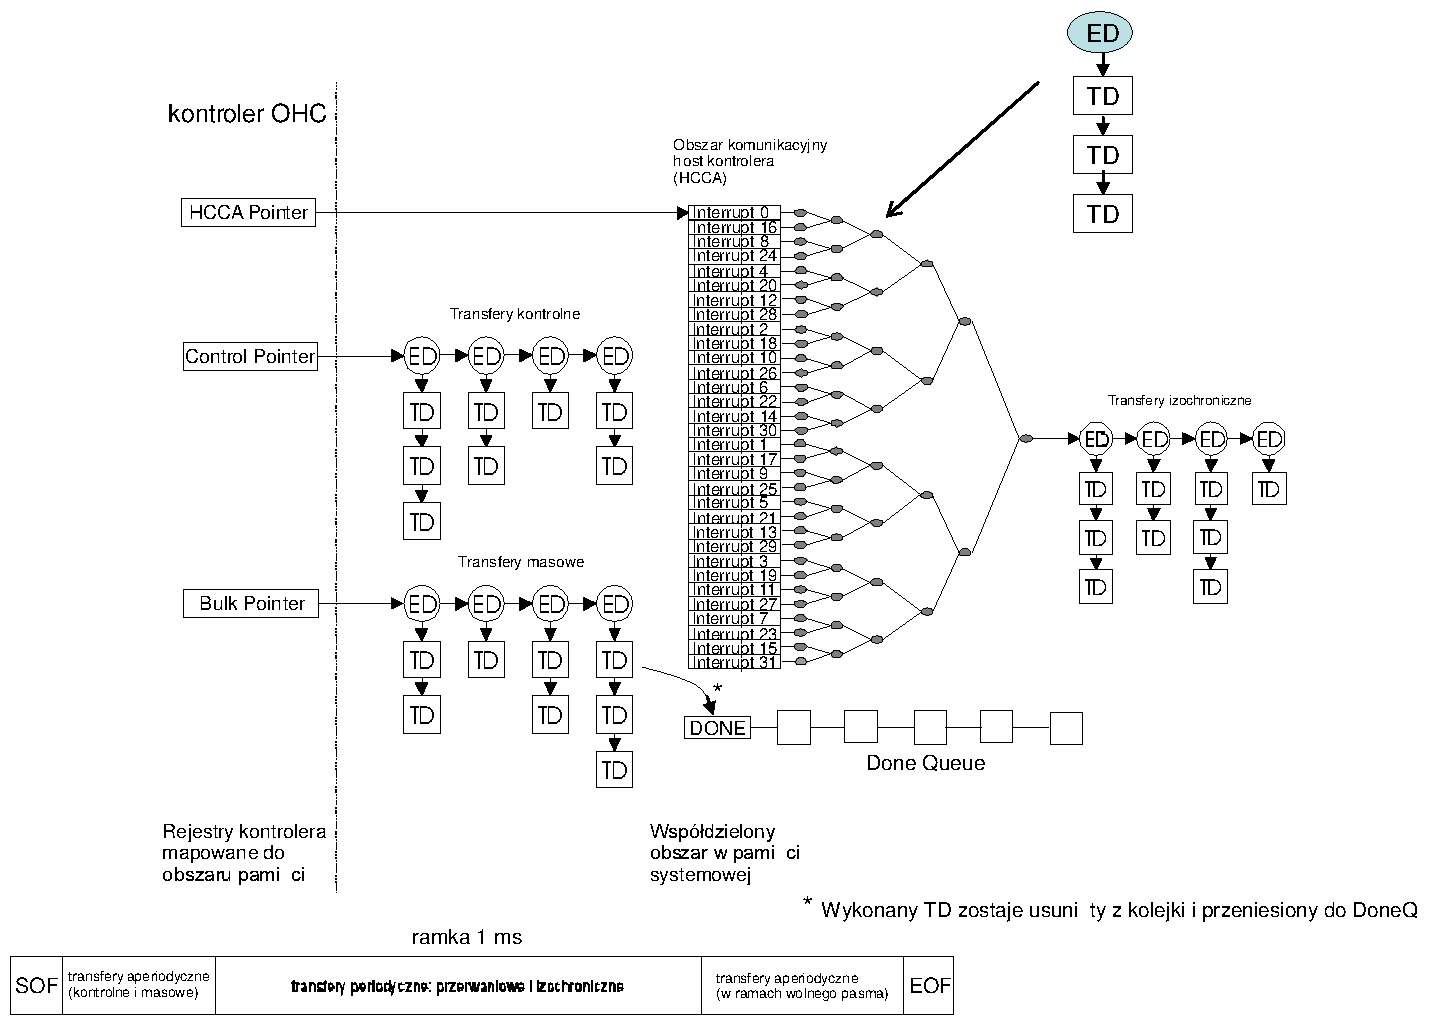
\includegraphics[width=7cm]{./wyklady/USB_49_1.pdf}\\\\
	\textbf{Format deskryptora punktu końcowego (ED)}\\
	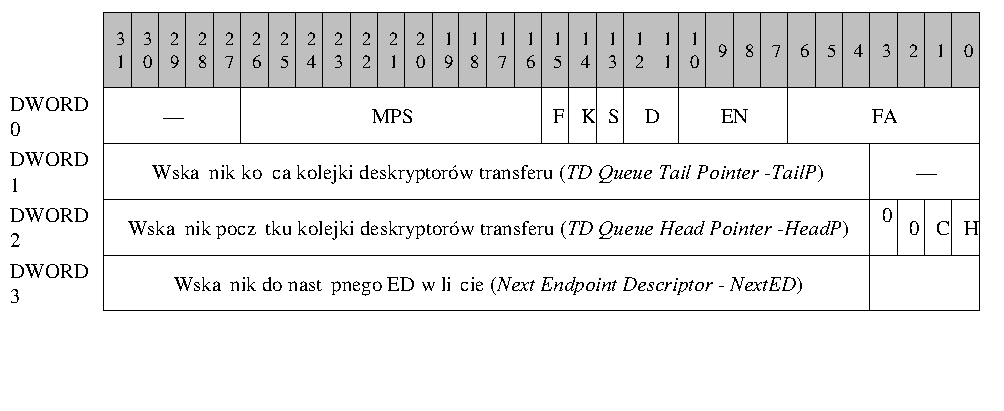
\includegraphics[width=7cm]{./wyklady/USB_50_1.pdf}\\\\
	\textbf{Ogólna postać deskryptora transferu (TD)}\\
	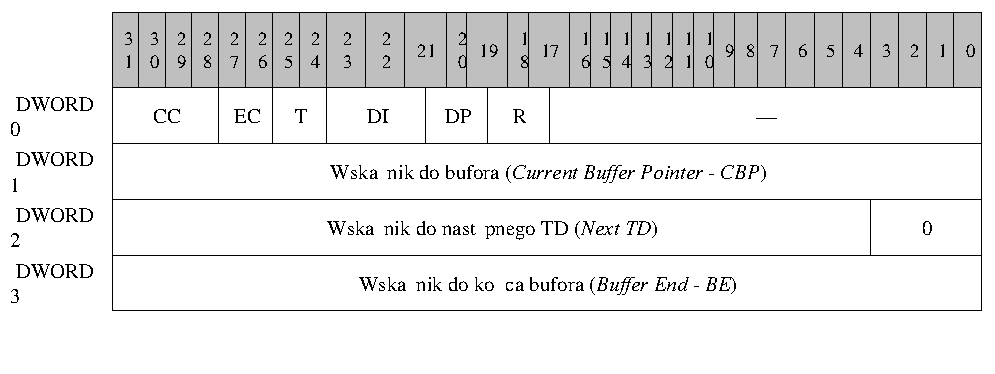
\includegraphics[width=7cm]{./wyklady/USB_51_1.pdf}
	
\subsection{USB 2.0 - rozszerzenie standardu}
	\subsubsection{Ważniejsze elementy wprowadzone w USB 2.0}
	\begin{itemize}
		\item Wysoka szybkość transmisji (high speed) - 480 Mb/s
		\item Protokół PING-NYET
		\item Transakcja SPLIT
		\item Komunikacja z szerokopasmowym punktem izochronicznym
		\item Nowe typy pakietów
	\end{itemize}
	\subsubsection{Wysoka szybkość transmisji}
	Podział ramki na 8 mikroramek wysokiej szybkości\\
	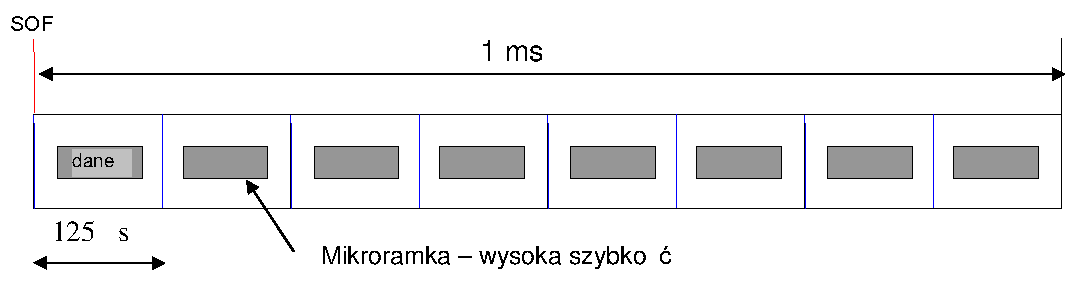
\includegraphics[width=7cm]{./wyklady/USB_53_1.pdf}
	\begin{itemize}
		\item Mikroramka trwa 125 $\mu s$
		\item Na 1 ramkę przypada 8 mikroramek
		\item Wysoka szybkość transmisji - w mikroramce wynosi 480 Mhz.
	\end{itemize}
	\subsubsection{Protokół PING-NYET}
	Potwierdzenie NYET (\emph{NOT YET}) dla urządzeń \emph{high speed}.\\
	\textbf{Problem:} przy zapisie do urządzenia, jeżeli nie jest ono „gotowe na dane” potwierdzenie negatywne przychodzi dopiero po pakiecie danych – strata czasu.\\
	\textbf{Rozwiązanie}:\\
	TOKEN PING – zapytanie urządzenia, czy jest gotowe do przyjścia danych.\\
	Możliwe odpowiedzi i reakcja hosta:
	\begin{itemize}
		\item ACK – wykonanie transakcji OUT
		\item NYRT – host kontynuuje wysyłanie zapyta PING
	\end{itemize}
	\textbf{Korzyści}: lepsze wykorzystanie magistrali (PING jest krótki).
	\subsubsection{Transakcja SPLIT}
	\textbf{Problem:} Host i hub wysokiej szybkości komunikują się z urządzeniem małej lub pełnej szybkości. Szybkie przesyłanie danych pomiędzy hostem i hubem oraz wolne pomiędzy hubem i urządzeniem – konieczność buforowania danych w hubie.\\
	\textbf{Rozwiązanie}:\\
	Transakcja dzielona, złożona z dwóch części:
	\begin{itemize}
		\item SSPLIT (\emph{Start Split} - rozpoczęcie transakcji dzielonej)
		\item CSPLIT (\emph{Complete Split} – zakończenie transakcji dzielonej).
		\item Pomiędzy tymi dwoma elementami transakcji dzielonej mogą być wykonywane inne transakcje z wysoką szybkością.
	\end{itemize}
	\subsubsection{Komunikacja z szerokopasmowym punktem izochronicznym}
	Komunikacja z „normalnym” izochronicznym punktem końcowym zakłada jedną transakcję na ramę lub mikroramkę.\\
	W przypadku punktów szerokopasmowych, obsługiwanych tylko przez kanały \emph{high speed}, istnieje możliwość przekazania w jednej mikroramce większej ilości danych wykonując bezpośrednio po sobie od jednej do trzech transakcji.\\
	Dane w takiej sekwencji transakcji muszą być oznaczone, przy czym nie wystarczą już „znaczniki” Data 0 i Data 1, dlatego wprowadzono dwa kolejne typy pakietów danych: \textbf{Data 2} i \textbf{MData}.\\
	Pakiet \textbf{Data 2} wykorzystywany jest przy odczycie danych z urządzenia, natomiast \textbf{MData} i \textbf{Data 2} przy zapisie do urządzenia.\\
	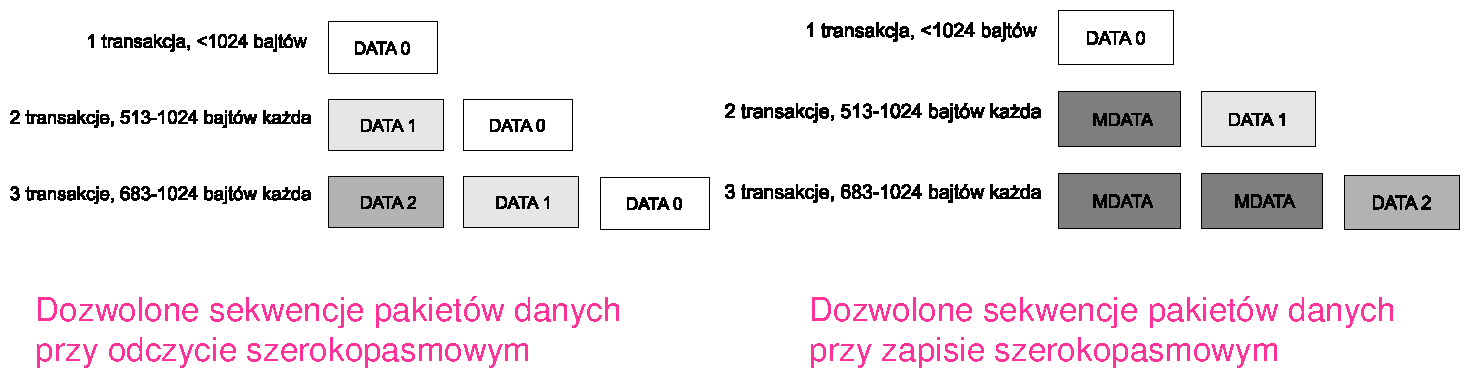
\includegraphics[width=15cm]{./wyklady/USB_56_1.pdf}
	\subsubsection{Specjalne pakiety TOKEN wprowadzone w USB 2.0}
	Kody pakietów specjalnych zgodnie z USB 2.0\\
	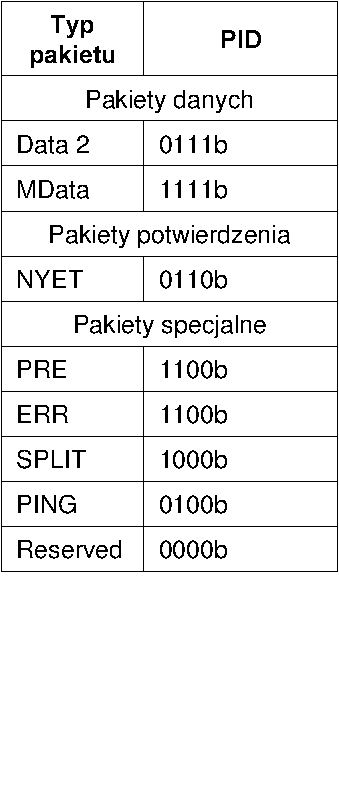
\includegraphics[width=3cm]{./wyklady/USB_57_1.pdf}
	
%IEE-488 i SCPI
% !TeX spellcheck = pl_PL
\newcommand\XOR{\mathbin{\char`\^}}

\section{IEEE-488 and SCPI standards}
Standard IEEE-488, ogłoszony w 1973 roku, określa organizację systemów ATE (\emph{Automatic Test Equipment}), przeznaczonych do akwizycji danych i sterowania urządzeń w obiektach skupionych lub rozproszonych. Te mają zastosowanie w testowaniu wyborów, pomiarach laboratoryjnych, sterowaniu procesami przemysłowymi itp.\\
Urządzenia systemu ATE wyposażone są w układ komunikacyjny (interfejs), który umożliwia wymianę danych za pomocą łącza interfejsowego. Pracą systemu zarządza kontroler, który jest nadrzędny w stosunku do pozostałych urządzeń, które pełnią rolę przyrządów wykonawczych.\\
Standard IEEE-488 znany jest również jako GPID (\emph{General Purpose Interface Bus}). Określa on dokładnie własności elektryczne i mechaniczne interfejsu, jego protokoły i funkcje, jednak nie normuje przesyłanych treści. Tym zajmuje się uzupełnienie standardu w postaci IEEE-488.2 (1973) oraz SCPI (1990).\\\\
Protokół systemu ATE można podzielić na 3 poziomy:
\begin{itemize}
	\item Poziom 1, złożony z
	\begin{itemize}
		\item Warstwa fizyczna (GPIB), określa łącze transmisyjne i sposób przesyłania jednostek
		\item Warstwa łącza danych, dostarcza reguły dostępu do łącza, sposób adresacji itp.
	\end{itemize}
	\item Poziom 2, IEEE-488.2 kontroler $<->$ IEEE-488.2 urządzenie\\
	Standard IEEE-488.2 okresla protokół wymiany komunikatów, syntaktykę komunikatów i strukturę danych.
	\item Poziom 3, rozkazy SCPI $<->$ Interpretacja rozkazów, generacja odpowiedzi\\
	SCPI normuje treść komunikatów przesyłanych pomiędzy kontrolerem a urządzeniem.
	\item Poziom 4, Aplikacja $<->$ Wykonanie funkcji urządzenia (ale to już nas raczej nie interesuje).
\end{itemize}
\textbf{Ilustracja rozwoju standardu IEEE-488} oraz \textbf{model komunikacyjny systemu ATE}\\
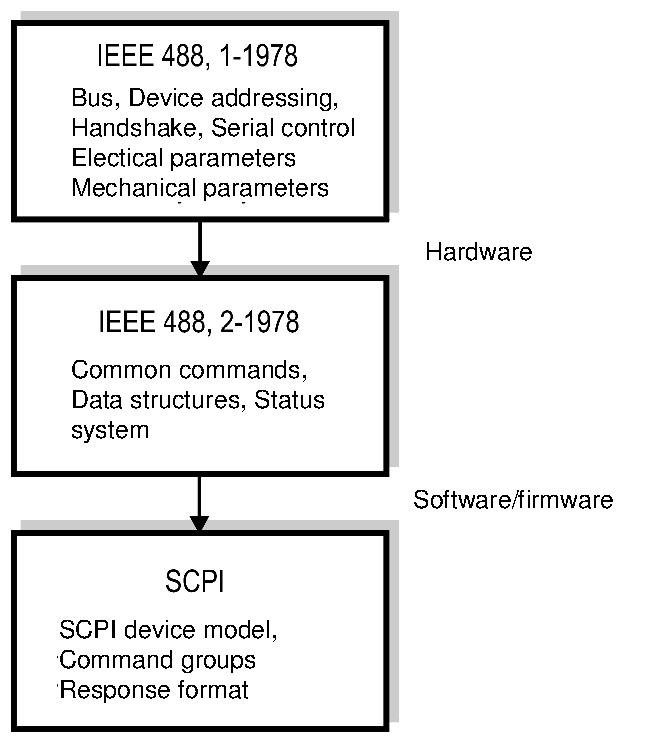
\includegraphics[width=7cm]{./wyklady/IEEE488_SCPI_17_1.pdf}
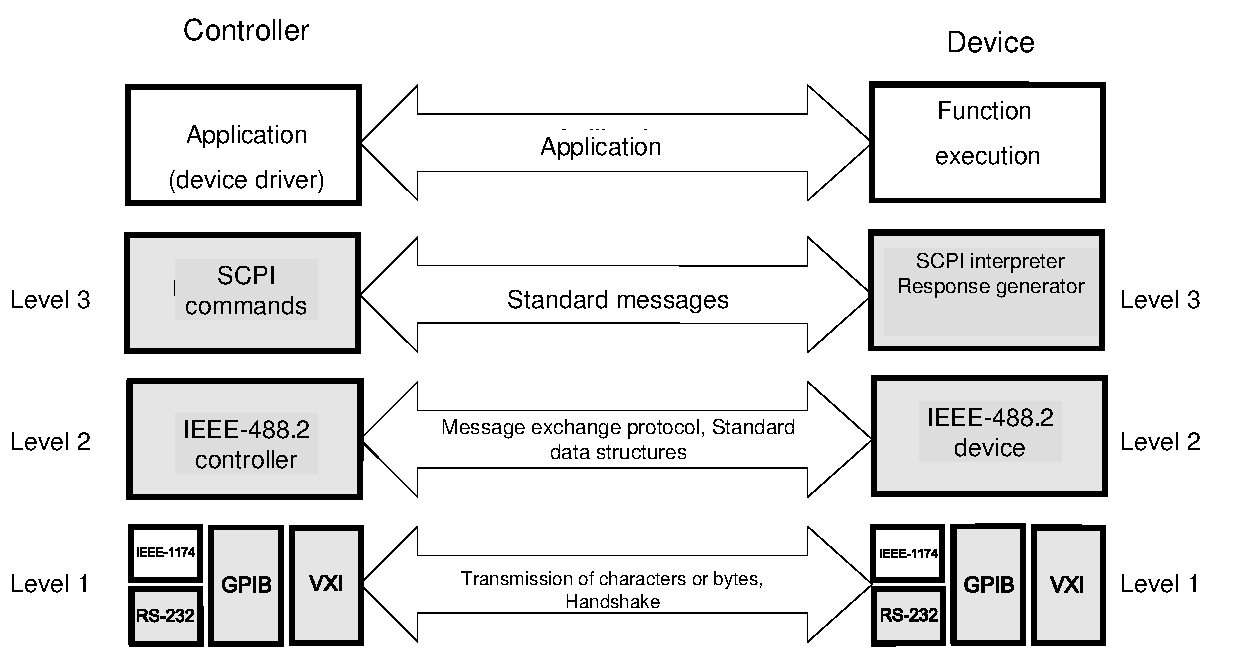
\includegraphics[width=9cm]{./wyklady/IEEE488_SCPI_18_1.pdf}

% ==============================================================
% --- Standard IEEE-488
% ==============================================================
\subsection{IEEE-488 (GPIB)}
Standard GPIB ogłoszono w 1979 roku, jest definicją warstwy fizycznej oraz łącza danych dla systemów pomiarowo-kontrolnych, przeznaczonych do:
\begin{itemize}
	\item Testowania wyborów
	\item Pomiarów laboratoryjnych i przemysłowych
\end{itemize}

\subsubsection{Interface profile}
Standard ten określa budowę i działanie części komunikacyjnej systemu opartego na magistrali, do której można:
\begin{itemize}
	\item Podłączyć do 15 urządzeń,
	\item Rozłożonych na niewielkim obszarze (zasięg do 20 m),
	\item Maksymalna odległość między kolejnymi urządzeniami to 2 m,
	\item Wymieniających między sobą dane rzędu 300 do 500 kB / s
\end{itemize}
Komunikacją zarządza kontroler, który konfiguruje system do komunikacji, obsługuje zgłoszenia żądania obsługi i wykonuje podstawowe operacje.
\textbf{Dwie podstawowe konfiguracje systemu GPIB}\\
\includegraphics[width=10cm]{./wyklady/IEEE488_SCPI_2_1.pdf}\\
\textbf{Podział urządzenia systemowego na cześć interfejsową i urządzenie właściwe}\\
Można tak podzielić każde urządzenie wykonawcze. Częsc interfejsowa to zdolność urządzenia do wymiany komunikatów z innymi elementami systemu, a urządzenie właściwe wykonuje podstawowe funkcje urządzenia.\\
\includegraphics[width=8cm]{./wyklady/IEEE488_SCPI_2_2.pdf}


\subsubsection{Magistrala}
\begin{wrapfigure}{r}{0.5\textwidth}
	\vspace{0pt}
	\begin{center}
		\includegraphics[width=0.40\textwidth]{./wyklady/IEEE488_SCPI_3_1.pdf}
	\end{center}
	\vspace{-20pt}
	\caption{Reprezentacja magistrali}
	\vspace{-10pt}
\end{wrapfigure}

\textbf{Właściwości}
\begin{itemize}
	\item Magistrala zawiera 16 linii
	\begin{itemize}
		\item 8 dla transmisji danych
		\item 8 dla sygnałów sterujących
	\end{itemize}
	\item Jest to łącze równoległe, umożliwia przesłanie wszystkich bitów bajtu
	\item DIO1-DIO8 – dwukierunkowa magistrala danych
	\item 5 sygnałów kontrolnych:
	\begin{itemize}
		\item ATN (\emph{Attention} - wyjście), określa tryb pracy magistrali danych
		\begin{itemize}
			\item ATN=0 - transmisja bajtów danych
			\item ATN=1 - transmisja instrukcji sterujących (adresów lub rozkazów)
		\end{itemize}
		\item REN (\emph{Remote Enable} – wyjście), 1 oznacza, że system jest zarządzany zdalnie przez kontroler
		\item IFC (\emph{Interface clear} – wyjście), 1 powoduje wyzerowanie części interfejsowych urządzeń
		\item SRQ (\emph{Service request} – wejście), 1 oznacza, że w systemie jest co najmniej jedno urządzenie żądające obsługi
		\item EOI (\emph{End Or Identity} – wyjście or wejście), zależny od stanu linii ATN
		\begin{itemize}
			\item EOI=1 razem z ATN=0 (EOI=1 $\XOR$ ATN=0) - realizacja znacznika końca bloku danych
			\item EOI=1 razem z ATN=1 (EOI=1 $\XOR$ ATN=1) – kontrola równoległa
		\end{itemize}
	\end{itemize}
	\item 3 sygnały sterujące (\emph{Byte handshake signals})
	\begin{itemize}
		\item NRFD (\emph{Not Ready For Data} – wyjście or wejście) - jest co najmniej jeden odbiorce niegotowy do przyjęcia danych
		\item DAV (\emph{Data Valid} – wyjście or wejście) - bajt znajdujący się na magistrali jest ważny i może zostać odczytany
		\item NDAC (\emph{Not Data Accepted} – wyjście or wejście) - przyjęcia bajtu na magistrali nie zostało potwierdzone przez wszystkich odbiorców
	\end{itemize}
\end{itemize}

\subsubsection{Funkcje interfejsowe}
Każda funkcja reprezentuje pewną określoną zdolność urządzenia jako jednostki systemu GPIB.\\
Ciekawostka: każda funkcja implementowana jest tylko w tych urządzeniach, które jej potrzebują.
\begin{itemize}
	\item SH (\emph{Source Handshake}) - inicjator transmisji, dla urządzeń mogących nadawać dane
	\item AH (\emph{Acceptor Handshake}) - akceptor transmisji, dla urządzeń mogących odbierać dane
	\item T (\emph{Talker}) - nadawca, umożliwienie wprowadzenia bajtu na magistralę danych
	\item L (\emph{Listener}) - odbiorca, umożliwienie odebranie bajtu z magistrali danych
	\item SR (\emph{Service Request}) - zgłoszenie żądania obsługi
	\item DC (\emph{Device Clear}) - zerowanie urządzenia, umożliwienie zdalnego zerowania (reset)
	\item DT (\emph{Device Trigger}) - wyzwalanie urządzenia, umożliwienie zdalnego wyzwolenia operacji (pomiaru)
	\item RL (\emph{Remote/Local}) - zdalne / lokalne, umożliwienie przełączania trybu urządzenia
	\item PP (\emph{Parallel Poll}) - kontrola równoległa
	\item C (\emph{Controller}) - kontroler, umożliwienie zdalnego zarządzania systemem GBIB i przekazywanie zarządzania innym kontrolerom - w systemie może być wiele kontrolerów, jednak tylko jeden może być aktywny, reszta musi być uśpiona.
\end{itemize}

\subsubsection{Podział komunikatów}
\includegraphics[width=10cm]{./wyklady/IEEE488_SCPI_8_1.pdf}\\\\
komunikaty dzielimy na zdalne(przesyłane po magistrali)  i lokalne (wymieniane między częścią interfejsowa, a urządzeniem właściwym).\\
Komunikaty zdalne dzielimy na:
\begin{itemize}
	\item wieloliniowe: przenoszone przez magistrale danych. Tutaj wyróżniamy:
	\begin{itemize}
		\item instrukcje sterujące (adresy lub rozkazy)
		\item dane
	\end{itemize}
	\item jednoliniowe: przenoszone przez wydzieloną linię sterującą
\end{itemize}

\textbf{Podział funkcjonalny komunikatów}:
\begin{itemize}
	\item UC (\emph{Universal Commands}) - rozkazy uniwersalne, przeznaczone dla wszystkich urządzeń w systemie
	\item AC (\emph{Addressed Commands}) - rozkazy adresowane, przeznaczona tylko na konkretnych urządzeń
	\item AD (\emph{Addresses}) - adresy, komunikaty umożliwiające wyznaczenie urządzenia nadającego i urządzeń odbierających
	\item HS (\emph{Handshake}) - komunikaty synchronizacji, kontrolujące transfer bajtu przez magistralę danych
	\item DD (\emph{Device Depended} (data)) - komunikaty zależne od urządzenia, ich znaczenie jest zależne od przyrządu
	\item ST (\emph{Status}) - komunikaty statusowe, udostępniają informacje o stanie urządzenia
	\item SE (\emph{Secondary}) - komunikaty wtórne, adres lub rozkaz wtórny
\end{itemize}

\subsubsection{Złącze interfejsu (connector)}
\begin{wrapfigure}{r}{0.5\textwidth}
	\vspace{0pt}
	\begin{center}
		\includegraphics[width=0.30\textwidth]{./wyklady/IEEE488_SCPI_11_1.pdf}
	\end{center}
	\vspace{-20pt}
	\caption{Złącze}
	\vspace{-10pt}
\end{wrapfigure}
W systemie GPIB zastosowano 24-stykowe złącze.
\begin{itemize}
	\item Wszystkie sygnały mają wspólny potencjał odniesienia (masę SG).
	\item Linie sterujące: DAV, NRFD, NDAC, IFC, SRQ oraz ATN są wykonane w postaci skręcanej pary przewodów, w któryc przewód powrotny jest podłączony odpowiednio do punktów TP1, TP2, ... TP11.
	\item Zacisk SHIELD stanowi kontakt do podłączenia ekranu kabla.
\end{itemize}

\subsubsection{Schemat blokowy interfejsu GPIB}
\includegraphics[width=10cm]{./wyklady/IEEE488_SCPI_12_1.pdf}

% ==============================================================
% --- Standard IEEE-488.2
% ==============================================================
\subsection{Standard IEEE-488.2}
Standard ten określa:
\begin{itemize}
	\item Protokół wymiany komunikatów pomiędzy kontrolerem, a urządzeniem na poziomie warstwy 2
	\item Synchronizację działania kontrolera i urządzenia
	\item Strukturę systemu statusowego w urządzeniu i sposób jego obsługi
	\item Zestaw tzw. rozkazów wspólnych
\end{itemize}

\subsubsection{Schemat funkcjonalny urządzenia}
Ilustracja przepływu danych i ich przetwarzania\\
\includegraphics[width=9cm]{./wyklady/IEEE488_SCPI_19_1.pdf}

\subsubsection{Protokół wymiany komunikatów}
Jego zadaniem jest zapewnienie poprawnego transferu wiadomości pomiędzy kontrolerem, a urządzaniem i określenie reakcji urządzenia na naruszenia reguł protokołu.\\
Ogółem komunikacja pomiędzy kontrolerem a urządzeniem polega na:
\begin{itemize}
	\item wysyłaniu do urządzenia komunikatów programujących, które można podzielić na rozkazy bez odpowiedzi i zapytania
	\item odbieraniu odpowiedzi z urządzenia na wysłane zapytania
\end{itemize}
\textbf{Zasady komunikacji kontrolera z urządzeniem (\emph{Device responsibility})}
\begin{enumerate}
	\item Rozkazy są wykonywane przez urządzenie zgodnie z kolejnością ich wprowadzenia do przyrządu (poza ściśle określonymi wyjątkami)
	\item Urządzenie jest zobowiązane odesłać odpowiedź tylko na wcześniej odebrane zapytanie (przez kontroler)
	\item Odpowiedzi na zapytania są odsyłane w kolejności odpowiadającej odebranym zapytaniom
\end{enumerate}
\textbf{Reguły protokołu komunikacyjnego (\emph{Controller responsibility})}
\begin{enumerate}
	\item Kontroler nie może odebrać odpowiedzi na zadane zapytanie, zanim nie zakończy rozpoczętego komunikatu programowego.
	\item Kontroler nie może wysłać kolejnego komunikatu programowego, jeżeli nie odebrał w całości wszystkich odpowiedzi na zadane wcześniej zapytania.
	\item Kontroler nie może podejmować próby odczytu odpowiedzi z urządzenia, jeżeli wcześniej nie wysłał żadnego zapytania.
	\item Zapytanie powodujące odesłanie odpowiedzi o nieokreślonym rozmiarze musi być umieszczone jako ostatnie zapytanie w komunikacie programowym (zawierającym kilka zapytań).
	\item Istnieje niebezpieczeństwo zablokowania urządzenia w przypadku wprowadzenia do urządzenia komunikatu programowego zawierającego kilka zapytań.
\end{enumerate}

% ==============================================================
% --- Standard SCPI
% ==============================================================
\subsection{Standard SCPI}
SCPI (\emph{Standard Commands for Programmable Instruments}), normalizuje treści komunikatów przepływających pomiędzy kontrolerem, a urządzeniem. Można go uważać za język kontroli, określono w nim budowę i reguły syntaktyczne komunikatów programowych wysyłanych do urządzenia i odpowiedzi z urządzenia.\\
Wywodzi się z normy IEEE-488.2.

\subsubsection{Budowa komunikatów}
komunikaty składają się z jednego lub kilku komunikatów jednostkowych. Na końcu komunikatu programowego musi wystąpić znacznik terminujący.\\
\includegraphics[width=10cm]{./wyklady/IEEE488_SCPI_21_2.pdf}\\\\
\textbf{Komunikat programowy}:
\begin{itemize}
	\item \textbf{Nagłówek}: tekst okreslający znaczenie komunikatu. Może to być pojedyncze słowo kluczowe lub ciąg słów oddzielonych znakiem dwukropka (':', 3Ah)
	\item \textbf{Separator nagłówka}: występuje pomiędzy nagłówkiem, a pierwszym parametrem jako jeden lub kilka znaków niedrukowalnych ASCII z zakresu od 0 do 31 (dec), oprócz NL, 0Ah. Najczęściej jest to jedna lub kilka spacji.
	\item \textbf{Parametry}: określają wartości związane z rozkazem. Separatorem pomiędzy parametrami jest znak przecinka (',', 2Bh), przy czym białe znaki sa ignorowane.
	\item \textbf{Separator komunikatów jednostkowych}: jest to znak średnika (';', 3Bh)
	\item \textbf{Terminator komunikatu}: znacznik terminujący, który jest wymagany do zakończenia komunikatu. Jest to znak LF (NL, 0Ah)
\end{itemize}
\textbf{Odpowiedź}:
\begin{itemize}
	\item Zawierają tylko dane,  
	\item a reszta jak w powyższym
\end{itemize}
\textbf{Zapytanie}:
\begin{itemize}
	\item Nagłówki zapytań mają na końcu znak pytajnika ('?', 3Fh)
\end{itemize}
\textbf{Komunikaty wspólne}:
\begin{itemize}
	\item Posiadają prefiks w postaci znaku gwiazdki ('*', 2Ah)
\end{itemize}
\textbf{Drzewiasta struktura rozkazów SCPI} (jest to to fragment drzewa podsystemu [SENSe]):\\
\includegraphics[width=9cm]{./wyklady/IEEE488_SCPI_22_1.pdf}

\subsubsection{Model urządzenia w standardzie SCPI}
Schemat blokowy ilustrujący przepływ sygnału i danych w urządzeniu. Poszczególne bloki reprezentują podstawowe funkcje urządzenia, a ich nazwy są jednocześnie nazwami grup rozkazów (podsystemów), które obsługują daną funkcjonalność.\\
\includegraphics[width=9cm]{./wyklady/IEEE488_SCPI_23_1.pdf}\\
Wyróżnia się dwie części:
\begin{itemize}
	\item akwizycję sygnału ("czujnik")
	\item generację sygnału ("źródło")
\end{itemize}

\subsubsection{Podsystemy w standardzie SCPI}
Podsystem to grupa funkcjonalności. W każdym konkretnym urządzeniu występują tylko te, które są mu potrzebne.\\
Owych podsystemów jest kilkanaście, tutaj są przedstawione najistotniejsze:
\begin{itemize}
	\item \textbf{CALCulate} - odpowiedzialny za matematyczne przetwarzanie wyników i danych po akwizycji sygnału lub przed generacją sygnału
	\item \textbf{INput} - przekształcanie sygnału (wzmocnieniem, filtracją itp.) przed właściwą konwersją dokonywaną w bloku SENSe
	\item \textbf{OUTput} - kontrola przekształtników sygnału wyjściowego (po generacji przez blok SOURce)
	\item \textbf{ROUTe} - odpowiedzialny za podłączenie sygnału wejściowego do układu przekształcającego sygnał lub wyjściowego do zacisków wyjściowych przyrządu
	\item \textbf{SENSe} - kontrola podstawowego modułu akwizycji sygnału (bloku wykonującego konwersję analogowo-cyfrową)
	\item \textbf{SOURce} - kontrola modułu generacji sygnału
	\item \textbf{SYSTem} - podsystem umożliwiający "utrzymanie" przyrządu (kontrolę pomocniczych parametrów)
\end{itemize}

\subsubsection{Parametry}
Typy parametrów w komunikatach programowych i odpowiedziach zostały określone w standardzie IEEE-488.2, natomiast w SCPI wyróżniono kilka klas parametrów w ramach wybranych typów IEEE-488.2.\\
\includegraphics[width=9cm]{./wyklady/IEEE488_SCPI_30_1.pdf}

\subsubsection{Kontrola urządzeń}
Urządzenie kontrolowane przez rozkazy SCPI\\
\includegraphics[width=10cm]{./wyklady/IEEE488_SCPI_16_1.pdf}


\subsubsection{System rejestrów statusu}
Urządzenie przechowuje informację o stanie w tzw. SRS, który ma strukturę hierarchiczną, złożoną z 5 grup rejestrowych. Każda z nich składa się z rejestru zdarzeń i rejestru maski.
\begin{enumerate}
	\item Bajt statusowy - umieszczona w najwyższym poziomie hierarchii, udostępnia uogólnioną informacje o stanie urządzenia.
	\item Rejestr zdarzeń standardowych - 8-bitowy rejestr na drugim poziomie hierarchii, informuje o wystąpieniu zdarzeń uważanych za "typowe" dla urządzenia SCPI.
	\item Rejestr znaczników urządzenia - 16-bitowy rejestr na drugim poziomie hierarchii, informuje o "jakości" wyników pomiaru i sprawności ważniejszych układów w przyrządzie.
	\item Rejestr operacji - 16-bitowy rejestr na drugim poziomie hierarchii informujący o stanie wykonywanych przez przyrząd operacji.
	\item Rejestr statusu zależny od urządzenia - specyficzny dla urządzenia, liczba i znaczenie bitów są od niego zależne.
\end{enumerate}
\includegraphics[width=9cm]{./wyklady/IEEE488_SCPI_32_1.pdf}\\\\
Minimal SCPI status system\\
\includegraphics[width=9cm]{./wyklady/IEEE488_SCPI_33_1.pdf}

\subsubsection{Synchronizacja urządzeń z aplikacją w standardzie SCPI}
Zadaniem synchronizacji jest zapewnienie właściwej sekwencji operacji urządzeń w systemie.\\
W urządzeniach SCPI synchronizacja aplikacji sterującej z operacjami wykonywanymi przez urządzenie oparta jest na rozkazach *OPC, *OPC? oraz *WAI.\\
\textbf{Rodzaje rozkazów}
Dzielimy je na:
\begin{itemize}
	\item Sekwencyjne - wykonywane jeden po drugim w kolejności wprowadzania ich do przyrządu.
	\item Nakładające się - możliwe wykonywanie wielu rozkazów jednocześnie.
\end{itemize}
\includegraphics[width=7cm]{./wyklady/IEEE488_SCPI_37_1.pdf}\\\\
\textbf{Rozkazy *OPC, *OPC? oraz *WAI}\\
\includegraphics[width=7cm]{./wyklady/IEEE488_SCPI_38_1.pdf}

\subsubsection{Wyzwalanie operacji (device trigger)}
Standard SCPI umożliwia uzależnienie wyzwolenia od spełnienie szeregu warunków i wystąpienia róznych zdarzeń (elastyczność).\\
Typowy układ wyzwalania operacji (trigger circuit in HP-34401A multimeter)\\
\includegraphics[width=7cm]{./wyklady/IEEE488_SCPI_39_1.pdf}


%FireWire
% !TeX spellcheck = pl_PL
\newpage
\section{IEEE-1394 (FireWire)}
Cel projektantów FireWire: stworzenie interfejsu opartego na łączu szeregowym, który mógłby zastąpić równoległy port SCSI. Chodziło o zaprojektowanie bardzo szybkiej magistrali, dogodnej do transferu dużej ilości danych wymienianych z urządzeniami pamięci masowych oraz danych multimedialnych.

\subsection{Możliwości interfejsu IEEE 1394a}
\begin{itemize}
	\item Podłączenie do komputera dużej liczby różnorodnych urządzeń
	\item Wykrywanie włączenia urządzenia do systemu oraz jego odłączenia (\emph{hot plugging})
	\item Automatyczna konfiguracja systemu do komunikacji
	\begin{itemize}
		\item określenie topologii systemu
		\item samoidentyfikacja urządzeń
		\item wyznaczenie szybkości transmisji
		\item konfiguracja urządzeń do komunikacji
	\end{itemize}
	\item Szybka transmisja danych pod kontrolą pakietowego protokołu komunikacyjnego, oparta na transakcjach asynchronicznych i izochronicznych
	\item Rywalizacyjny dostęp urządzeń do łącza pod kontrolą procedury arbitrażowej
	\item Zasilanie urządzenia z systemu
\end{itemize}

\subsection{Topologia i interfejs IEEE 1394a}
Układem umożliwiającym podłączenie komputera opartego na PCI do magistrali szeregowej IEEE 1394 jest most (\emph{Open Host Controller Interface}), który udostępnia zazwyczaj kilka portów IEEE 1394.\\
\includegraphics[width=10cm]{./wyklady/FIREWIRE_2_1.pdf}\\
\begin{itemize}
	\item Topologia rozgałęzionej gwiazdy.
	\item Struktura: rozgałęziona magistrala (\emph{daisy chain}).
	\item Poszczególne urządzenia, zwane węzłami, rywalizują ze sobą o dostęp do łącza w celu przesłania porcji danych (pakietu). Pakiety przesyłane są co 125 $\mu s$
	\item \textbf{Urządzenia z jednym portem stanowią zakończenie gałęzi} (liście), urządzenia z wieloma portami umożliwiają rozbudowę gałęzi przez podłączenie kolejnego urządzenia. Liściem może też być urządzenie wieloportowe , w którym wykorzystany jest tylko jeden port.
	\item \textbf{Komunikacja pomiędzy portami oparta jest na zasadzie punkt-punkt} (\emph{point to point}), co dla urządzenia wieloportowego oznacza odbiór i detekcję całego pakietu przez jeden port, a następnie jego resynchronizację do lokalnego zegara i retransmisję do pozostałych portów.
	\item \textbf{System nie posiada hosta}, komunikacja pomiędzy urządzeniami odbywa się bez interwencji stacji nadrzędnej. Ten rodzaj komunikacji określamy jako P2P (\emph{peer to peer})
	\item \textbf{Konfiguracja urządzeń następuje dynamicznie}, bez wykorzystania kontrolera systemu. Interfejsy urządzeń mają wbudowane funkcje konfiguracyjne, które umożliwiają określenie topologii systemu, parametryzację portów urządzeń oraz przekazanie informacji o urządzeniu. Odbywa się po każdym resecie.
\end{itemize}


\subsection{Architektura węzła}
System IEEE 1394 ma topologię rozgałęzionej gwiazdy i oparty jest na transferach bezpośrednich między urządzeniami (brak hosta w systemie).
\includegraphics[width=7cm]{./wyklady/FIREWIRE_3_1.pdf}\\
Ważniejsze terminy stosowane w IEEE 1394:
\begin{itemize}
	\item moduł (\emph{module}): fizyczne urządzenie podłączone do magistrali, które może zawierać kilka węzłów
	\item węzeł (\emph{node}): logiczne urządzenie wewnątrz modułu
	\item jednostka (\emph{unit}): element węzła o określonej funkcjonalności (np. procesor, pamięć, I/O)
\end{itemize}

\subsection{Przestrzeń adresowa i jej podział}
Przestrzeń adresowa jest zgodna z IEEE Std 1212-1991 Control and Status Register (CSR) Architecture.\\
\begin{itemize}
	\item Adres zawiera 64 bity podzielone na:
	\begin{itemize}
		\item Numer magistrali (\emph{Bus Number}), 10 najstarszych bitów: Bus 0 do Bus 1023
		\item Numer węzła w ramach magistrali (\emph{Node Number}), 6 bitów: Node 0 do Node 63
		\item Pole adresowe w węźle (\emph{Node Address}), 48 bitów.
	\end{itemize}
	\item Format adresu\\
	\includegraphics[width=10cm]{./wyklady/FIREWIRE_4_1.pdf}
	\item Podział pamięci węzła\\
	\includegraphics[width=10cm]{./wyklady/FIREWIRE_5_1.pdf}
\end{itemize}


\subsection{Transfery i transakcje}
Zasady komunikacji:
\begin{itemize}
	\item Transfery są żądaniami przesłania danych.
	\item Transfery dzielone są na transakcje (w celu umożliwienia podziału pasma pomiędzy węzłami).
	\item Wyróżnia się transakcje:
	\begin{itemize}
		\item \textbf{Asynchroniczne} - wymagają potwierdzenia (odpowiedzi) i w przypadku błędów są powtarzane. Mogą być wykonywane cyklicznie lub aperiodyczne.
		\item \textbf{Izochroniczne} - nie są potwierdzane. Nie kontroluje się poprawności przesłania danych, a jedynie zapewnia stały rytm ich dostarczania.
	\end{itemize} 
\end{itemize}

	\subsubsection{Transakcje asynchroniczne}
	\includegraphics[width=10cm]{./wyklady/FIREWIRE_7_1.pdf}\\
	Rozpoczęcie transakcji nie jest synchronizowane z odbiorcą. Wyróżniono 3 rodzaje transakcji asynchronicznych:
	\begin{itemize}
		\item Odczyt (\emph{read}) - pobranie danych od odbiorcy
		\item Zapis (\emph{write}) - przekazanie danych do odbiorcy
		\item Zamknięcie (\emph{lock}) - odczyt danych, ich modyfikacja i ponowny zapis
	\end{itemize}
	Każdą transakcję rozpoczyna inicjator transakcji (\emph{requester}) i potwierdza odbiorca transakcji (\emph{responder}). Zatem transakcja dzielona jest na dwie części:
	\begin{itemize}
		\item Fazę przekazania żądania (adres, rozkaz i dane)
		\item Fazę przekazania odpowiedzi (przy zapisie - status wykonania, przy odczycie - dane)
	\end{itemize}
	
	\subsubsection{Transakcje izochroniczne}
	\includegraphics[width=10cm]{./wyklady/FIREWIRE_8_1.pdf}\\
	\begin{itemize}
		\item Transfer izochroniczny zapewnia regularne dostarczanie danych bez sprawdzania ich ważności.
		\item Dane dostarczane są cyklicznie w odstępach 125 $\mu{s}$, bez potwierdzenia ich odbioru przez urządzenie odbierające.
		\item Życie danych izochronicznych jest wyjątkowo krótkie, a ich uszkodzenia nie mają trwałych konsekwencji.
		\item Przykładem mogą być dane cyfrowe reprezentujące dźwięk przesyłane do głośników.
	\end{itemize}

\subsection{Konfiguracja urządzeń do komunikacji, współdzielenie magistrali}
\subsubsection{Konfiguracja}
Po każdym włączeniu zasilania lub zmianie węzłów w systemie (dołączenie lub odłączenie urządzenia) następuje automatyczna konfiguracja magistrali, której rezultatem jest przygotowanie węzłów do działania.\\
Po przeprowadzeniu konfiguracji węzły mogą rywalizować o dostęp do magistrali (arbitraż), a po jego uzyskaniu przekazywać dane.
\subsubsection{Współdzielenie magistrali}
Transakcje asynchroniczne i izochroniczne współdzielą magistralę, ponieważ zarządzanie magistralą „stara się” umożliwić jednoczesne (quasi) jej wykorzystanie przez różne transfery.\\
\includegraphics[width=10cm]{./wyklady/FIREWIRE_13_1.pdf}\\
\newpage
\subsection{Model komunikacyjny}
Podstawowe funkcje warstw protokołu komunikacyjnego:
\begin{itemize}
	\item \textbf{Warstwa zarządzania magistralą} - konfiguracja i zarządzanie węzłem
	\item \textbf{Warstwa transakcji} - świadczy usługi dla transferów asynchronicznych realizując protokół żądanie-odpowiedź określony przez architekturę CSR. Wspiera 3 rodzaje operacji: odczyt, zapis i zamknięcie.
	\item \textbf{Warstwa połączeniowa} - wykonuje transakcję generując sekwencję pakietów w stacji nadrzędnej i odbierającej.
	\item \textbf{Warstwa fizyczna} - zapewnia elektryczny i mechaniczny interfejs szeregowej magistrali oraz wykonuje arbitraż w celu udostępnienia łącza tylko jednemu nadawcy (ochrona przed kolizją).
\end{itemize}
\includegraphics[width=10cm]{./wyklady/FIREWIRE_13_1.pdf}

	\subsubsection{Warstwa zarządzania magistralą}
	Zarządzanie magistralą obejmuje automatyczną konfiguracje węzła do komunikacji oraz, opcjonalnie, zarządzanie dystrybucją zasilania.\\
	Zarządzenia globalne obejmuje:
	\begin{itemize}
		\item przypisanie numeru kanału i pasma transferom izochronicznym
		\item kontrolę odstępów czasowych wykonywania transakcji izochronicznych
		\item kontrolę zasilania węzłów
		\item "dostrajanie" magistrali w celu polepszenia wydajności
		\item świadczenie usług dla innych węzłów, jak np. ustawienie maksymalnej szybkości transmisji pomiędzy węzłami
	\end{itemize}
	
	\subsubsection{Warstwa transakcji}
	Świadczy usługi dla transferów asynchronicznych, które umożliwiają:
	\begin{itemize}
		\item wykonanie odczytu z urządzenia (\emph{read})
		\item wykonanie zapisu danych do urządzenia (\emph{write})
		\item wykonanie modyfikacji danych w urządzeniu (\emph{lock})
	\end{itemize}
	Inicjatorem transakcji jest warstwa aplikacji, która zleca jej wykonanie warstwie transakcji. Model wykonania transkcji wyróżnia inicjatora (\emph{requester}) oraz odbiorcę (\emph{responder}), a także dzieli transakcję na dwie operacje: wysłanie żądania i odebranie odpowiedzi.
	\newpage
	Transakcja asynchroniczna z potwierdzeniem żądania i odpowiedzi (pakietów).\\
	\includegraphics[width=8 cm]{./wyklady/FIREWIRE_8_1.pdf}
	
	\subsubsection{Warstwa połączeniowa}
	Oparta na modelu żądanie-odpowiedź.
	\begin{itemize}
		\item Dla transferów asynchronicznych
		\begin{itemize}
			\item Warstwa połączeniowa węzła inicjującego transakcję dokonuje translacji żądania wykonania transakcji na pakiety przekazywane do warstwy fizycznej.
			\item Warstwa połączeniowa węzła odbierającego dokonuje operacji odwrotnej - przekształca odebrane z warstwy fizycznej pakiety i przekazuje je do warstwy transakcji.
		\end{itemize}
		\item Dla transferów izochronicznych jest podobnie, tylko żądanie wykonania transakcji (w węźle inicjującym) przekazywane jest do warstwy połączeniowej bezpośrednio przez sterownik programowy, a pakiety w warstwie połączeniowej u odbiorcy przekazywane są bezpośrednio do sterownika programowego.
	\end{itemize}
	Warstwa połączeniowa wykonuje również transakcje specjalne:
	\begin{itemize}
		\item Transakcja dzielona (\emph{Split Transaction}) - rozpoczęcie kolejnej transakcji przed zakończeniem poprzedniej. Pozwala na lepsze wykorzystanie magistrali i niezablokowanie jej.\\
		\includegraphics[width=10cm]{./wyklady/FIREWIRE_10_1.pdf}
		\item Transakcja dołączana (concatetated transaction) - umożliwia wykorzystanie magistrali przez inne węzły podczas gdy odbiorca transakcji opóźnia odesłanie odpowiedzi. Kiedy odpowiedź będzie już gotowa, odbiorca musi na drodze arbitrażu uzyskac dostęp do łącza (co wydłuża transakcję).\\
		Jeżeli jednak odbiorca jest zdolny do szybkiego udzielania odpowiedzi, może ją dołączyć do pakietu potwierdzenia wysyłanego w fazie przekazania żądania), co sprawia, że odbiorca transakcji nie musi rywalizować o dostęp do magistrali. Jest to transakcja dołączana.
		\item Transakcja zespolona (Unified Transaction) - to samo co transakcja dołączana, tylko ograniczona do operacji zapisu. Umożliwia włączenie odpowiedzi do potwierdzenia zamykającego fazę przekazania żądania. Sprawia to, że faza przekazania odpowiedzi jest niepotrzebna.\\
		\includegraphics[width=10cm]{./wyklady/FIREWIRE_11_1.pdf}
	\end{itemize}
	\subsubsection{Warstwa fizyczna}
	Prosty węzeł systemu IEEE 1394 z dwoma portami i liniami sygnałowymi magistrali.\\
	\includegraphics[width=10cm]{./wyklady/FIREWIRE_15_1.pdf}\\\\
	Podstawowe operacje realizowane na liniach sygnałowych:
	\begin{itemize}
		\item \textbf{Konfiguracja} - wykonywana po włączeniu zasilania oraz dołączeniu urządzania do magistrali bądź odłączenia z niej. Przygotowuje (wszystkie) węzły systemu do wymiany informacji.
		\item \textbf{Arbitraż} - konieczny jeżeli w toku jest kilka transakcji realizowanych przez różne węzły. Rywalizują one o dostęp do magistrali, a konflikt rozstrzyga procedura arbitrażowa. Konieczny przed przekazywaniem pakietu żądania i odpowiedzi, niekonieczny dla pakietu potwierdzenia.\\
		\includegraphics[width=10cm]{./wyklady/FIREWIRE_15_2.pdf}
		\item Przesył danych - prawo tego urządzenia, kto wywalczyło dostęp do magistrali. Dane kodowane są w zapisie NRZ (\emph{Non Return to Zero}).
	\end{itemize}
	\textbf{Szybkość transmisji}\\
	\includegraphics[width=7cm]{./wyklady/FIREWIRE_16_1.pdf}\\
	Minimum musi być spełnione! Szybkość transmisji może być większa, ale nie musi.
	Prędkości dla omawianych standardów:
	\begin{itemize}
		\item Dla IEEE 1394: S100
		\item Dla IEEE 1394a: S100, S200, S400
		\item Większe szybkości istnieją dla nowszych standardów
	\end{itemize}
	\newpage
	\textbf{Transakcja asynchroniczna}\\
	Jest to transakcja odczytu pomiędzy węzłami A i B (aplikacja w węźle B udostępnia dane tej w A).\\
	\includegraphics[width=7cm]{./wyklady/FIREWIRE_17_1.pdf}
	\includegraphics[width=7cm]{./wyklady/FIREWIRE_18_1.pdf}\\\\
	\textbf{Transakcja izochroniczna}\\
	Wykonywane pomiędzy aplikacją, a warstwą połączeniową, z pominięciem warstwy transakcji. Brak potwierdzania pakietów. Często mają charakter rozgłoszenia.\\
	\includegraphics[width=7cm]{./wyklady/FIREWIRE_19_1.pdf}\\\\
	Pakiety w transakcjach izochronicznych.\\
	Transakcje izochroniczne są jednokierunkowe i ograniczają się tylko do przekazania danych przez węzeł inicjujący transakcję. Odbiorca nie odsyła żadnej odpowiedzi. Znaczenie pól typowej transakcji izochronicznej:
	\begin{wrapfigure}{l}{8cm}
		\includegraphics[width=8cm]{./wyklady/FIREWIRE_20_1.pdf}
	\end{wrapfigure}
	\begin{itemize}
		\item Numer kanału (Channel Number) – węzły uczestniczące w transakcji izochronicznej wykorzystują numer kanału jako adres,
		\item Rodzaj transakcji(Transaction Type) – definiuje rodzaj przesyłanego pakietu jako „izochroniczny”.
		\item Dane (Data) – przekazywane dane,
		\item CRC – suma kontrolna.
	\end{itemize}
	\clearpage
	
	
\subsection{Interfejs fizyczny}
Obejmuje złącza, okablowanie  oraz układ elektryczny, spełnia funkcje takie jak:
\begin{itemize}
	\item nadawanie i odbiór sygnałów
	\item generacja i rozpoznawanie stanów interfejsu
	\item sygnalizacja maksymalnej szybkości transmisji akceptowanej przez dany port
\end{itemize}
W skład interfejsu fizycznego wchodzi również układ dystrybucji zasilania (umożliwia zasilanie węzłów, które nie mają własnych jednostek zasilających).\\
\includegraphics[width=9cm]{./wyklady/FIREWIRE_21_1.pdf}\\\\
W złączach zaciski zasilania są trochę wysunięte do przodu, co sprawia, że przy wdzióbywaniu najpierw doprowadzane jest zasilanie, a potem pojawia się kontakt na liniach sygnałowych.

\subsection{Interfejs sygnałowy}
Interfejs sygnałowy jest bardzo rozbudowy, ponieważ służy nie tylko do transmisji i odbioru danych, ale także do realizacji funkcji arbitrażowych.\\
\textbf{Sygnał różnicowy} - napięcie pomiędzy TPA/TPA*, a TPB/TPB*.\\
\textbf{Stan z} - oznacza stan trafny do wykrycia (nieokreślony). Jego pojawienie się na linii odczytywane jest jako cisza. \\

\textbf{Uproszczony schemat układów interfejsowych}\\
\includegraphics[width=9cm]{./wyklady/Rysunek01.pdf}
\newpage
\textbf{Odczytywanie stanu na linii połączeniowej} \\
\begin{tabular}{|c|c|c|}
	\hline Stan nadajnika nr 1 & Stan nadajnika nr 2 & Stan odczytywany na linii \\ 
	\hline 1 & 1 & 1 \\ 
	\hline 1 & 0 & Z \\ 
	\hline 1 & Z & 1 \\ 
	\hline 0 & 1 & Z \\ 
	\hline 0 & 0 & 0 \\ 
	\hline 0 & Z & 0 \\ 
	\hline Z & 1 & 1 \\ 
	\hline Z & 0 & 0 \\ 
	\hline Z & Z & Z \\ 
	\hline 
\end{tabular} 
\begin{itemize}
	\item TPA/TPA* - linia do przekazywania Strobe
	\item TPB/TBP* - linia do transmisji danych
\end{itemize}
Kodowanie bitów odbywa się w zapisach RZ (\emph{Return to Zero}) oraz NRZ (\emph{Non Return to Zero}).\\
Poniżej odtworzony zegar w interfejsie IEEE 1394. Zegar w węźle odbierającym jest przesunięty czasowo w stosunku do sygnałów Data i Strobe na wyjściu węzła nadającego, ponieważ sygnały ulegają opóźnieniom podczas transmisji w kablu.\\
\includegraphics[width=9cm]{./wyklady/FIREWIRE_28_1.pdf}\\\\
Zasada: w wyniku sumowania XOR bitów Data i Strobe uzyskać ciąg występujących na przemian 0 i 1, czemu odpowiada sygnał impulsowy o współczynniku wypełnienia 0.5 i półokresie odpowiadającym bitowej szybkości transmisji.\\\\
\textbf{Sygnalizacja arbitrażu} obejmuje 5 funkcji:
\begin{itemize}
	\item reset magistrali
	\item identyfikacja drzewa
	\item identyfikacja węzła
	\item normalny arbitraż
	\item pakiety startowy i końcowy
	\item sterowanie stanem portu (od wersji 1394a)
\end{itemize}
\textbf{Przerwy czasowe} - pomiędzy poszczególnymi fazami składającymi się na transakcję potrzebne są przerwy czasowe podczas których magistrala pozostaje w stanie jałowym.\\
\includegraphics[width=9cm]{./wyklady/FIREWIRE_29_1.pdf}\\
\begin{itemize}
	\item \textbf{Przerwa przed potwierdzeniem} - czas pomiędzy zakończeniem asynchronicznego pakietu (żądania lub odpowiedzi), a rozpoczęciem transmisji pakietu potwierdzenia.
	\item \textbf{Przerwa izochroniczna} - przeznaczona dla kanałów izochronicznych, zapewnia stan jałowy przed rozpoczęciem arbitrażu węzłów izochronicznych. krótsza niż przerwa dla kanałów asynchronicznych.
	\item \textbf{przerwa pomiędzy subakcjami} - dla kanałów asynchronicznych, zapewnia stan jałowy przed rozpoczęciem arbitrażu węzłów izochronicznych. Nie występuje między żądaniem a odpowiedzią w przypadku transmisji dołączanej.
	\item \textbf{Przerwa po resecie arbitrażu} - poprzedza "Interwał równych szans".
\end{itemize}

\subsection{Detekcja szybkości transmisji}
Ze względu na szybkość transmisji wyróżnia się 3 rodzaje portów:
\begin{itemize}
	\item transmisja tylko z szybkością podstawową S100
	\item transmisja z szybkością S100 lub S200
	\item transmisja z szybkością S100, S200 lub S400
\end{itemize}
Gdzie
\begin{itemize}
	\item S100 = 98.304 Mb/s
	\item S200 = 196.608 Mb/s
	\item S400 = 393.216 Mb/s
\end{itemize}
Tylko szybkość S100 jest obligatoryjna dla węzłów. Pozostałe dwa mogą, ale muszą być dostępne. Jeżeli jednak są, to wymagane są układy sygnalizacji szybkości transmisji.\\
Informacja o możliwych szybkościach transmisji każdego węzła przekazywana jest do innych węzłów rezydujących na magistrali podczas konfiguracji (w szczególności informacja o maksymalnej szybkości transmisji przekazywana jest do węzła podłączonego do tego samego segmentu kabla).\\
Zasadą jest nieprzekazywanie przez węzeł pakietów otrzymywanych z daną szybkością do podłączonych do niego węzłów o mniejszej szybkości.\\
Węzeł może mieć kilka portów, przez niektóre porty może być połączony z węzłami o szybkości większej od podstawowej, a przez inne z węzłami o szybkości podstawowej (zatem możliwa jest sytuacja, gdy węzeł odbiera pakiet z szybkością większą od podstawowej, przekazywany przez inny "szybki" węzeł, ale nie będzie go mógł przekazać do węzłów "wolniejszych").\\
\includegraphics[width=7cm]{./wyklady/FIREWIRE_31_1.pdf}

\subsection{Dystrybucja zasilania}
Węzły w systemie IEEE 1394 mogą być źródłem zasilania dla innych węzłów, korzystać z zasilania przez inne węzły lub też wykorzystywać zasilanie własne bez udostępniania go innym węzłom.\\
\subsubsection{Klasa zasilania}
Węzły wysyłają informację o zasilaniu w ramach pakietu „samoidentyfikacji” (\emph{self-ID}) podczas procesu konfiguracyjnego. Informacja ta przedstawia zapotrzebowania na zasilanie lub możliwość dostarczenia zasilania.\\
Informacje o zasilaniu przekazywane są na 3 bitowym polu \textbf{pwr} w pakiecie self-ID.\\
\includegraphics[width=9cm]{./wyklady/FIREWIRE_32_1.pdf}
\subsubsection{Dystrybucja zasilania}
Jeden lub kilka węzłów może jednocześnie być źródłem zasilania. Ponieważ napięcia zasilania udostępniane przez węzły mogą się różnić konieczna jest dioda zapobiegająca przepływowi prądu zasilania do węzła o mniejszym napięciu.\\
\includegraphics[width=8cm]{./wyklady/FIREWIRE_33_1.pdf}


\subsection{Arbitraż}
W FireWire węzły rywalizują o prawo do nadawania w ramach arbitrażu. Arbitraż realizowany jest w okresach przerw w transmisji (\emph{gaps}) i polega na:
\begin{itemize}
	\item Zagwarantowaniu pasma dla kanałów izochronicznych,
	\item Równoprawnej rywalizacji w przypadku kanałów asynchronicznych.
\end{itemize}
Arbitraż rozpoczyna się po rozpoznania przez węzeł okresu jałowego magistrali, co oznacza koniec poprzedniej transmisji. Czasy trwania jałowych stanów magistrali są różne dla transakcji izochronicznych i asynchronicznych i wynoszą:
\begin{itemize}
	\item Przerwa po resecie arbitrażu: 20 $\mu{s}$
	\item Przerwa pomiędzy subakcjami: 10 $\mu{s}$
	\item Przerwa przed potwierdzeniem: 40 ns
	\item Przerwa izochroniczna - od 40 ns (min) do 50 ns (max),
	\item Przerwa pomiędzy subakcjami transakcji asynchronicznej i przerwa przed potwierdzeniem mogą być „regulowane” (aby arbitraż rozpoczynał się jak najszybciej).
\end{itemize}
Sposób sygnalizowania arbitrażu (protokół sygnalizacji arbitrażu) jest taki sam dla transakcji asynchronicznych i izochronicznych.
\subsubsection{Rodzaje arbitrażu}
Typ pakietu, który jest przygotowany do transmisji, determinuje rodzaj żądania wykorzystywanego przez warstwę połączeniową. Są 4 rodzaje:
\begin{itemize}
	\item  arbitraż oparty na równej szansie dostępu do łącza (\emph{fair arbitration service}) stosowany przy transmisji pakietu asynchronicznego
	\item  arbitraż uwzględniający priorytety (\emph{proirity arbitration service}) stosowany przy transmisji pakietu cycle strat lub pakietu asynchronicznego o wyższym priorytecie
	\item  arbitraż natychmiastowy (\emph{immediate arbitration service}) stosowany przy transmisji pakietu potwierdzenia
	\item  arbitraż izochroniczny (\emph{isochronous arbitration service}) stosowany przy transmisji pakietu izochronicznego
\end{itemize}
\subsubsection{Przykład arbitrażu}
\includegraphics[width=8cm]{./wyklady/FIREWIRE_36_1.pdf}
\includegraphics[width=8cm]{./wyklady/FIREWIRE_37_1.pdf}\\
\includegraphics[width=9cm]{./wyklady/FIREWIRE_38_1.pdf}\\
\subsubsection{Arbitraż asynchroniczny}
\textbf{Zasada równych szans}
\begin{itemize}
	\item Węzły asynchroniczne do wykonania transakcji nie wymagają alokacji pasma.
	\item Działanie węzłów asynchronicznych polega na rotacyjnym przekazywaniu priorytetu (\emph{fairness interval} - „interwał równych szans”).
	\item Węzły asynchroniczne, które mają rozpoczęte transakcje uzyskują dostęp do magistrali w celu wykonania asynchronicznej subakcji (przesłania jednego pakietu).
	\item Kolejność przydziału zależy od położenia węzła w drzewie systemu. Węzły położone bliżej korzenia uzyskają dostęp przed węzłami bardziej oddalonymi.
	\item Łączny czas wykonania subakcji przez wszystkie węzły nazywa się \emph{fairness interval}.
	\item W tym czasie każdy węzeł uzyska dostęp do magistrali, aby wykonać subakcję.
	\item Dostęp do magistrali węzeł zarządzający przekazuje „rotacyjnie”.
	\item Następna subakcja będzie mogła być wykonana w kolejnym interwale równych szans.
\end{itemize}
\includegraphics[width=9cm]{./wyklady/FIREWIRE_40_1.pdf}\\\\
\textbf{Odesłanie potwierdzenia, dostęp natychmiastowy}
\begin{itemize}
	\item Węzeł, który zainicjował asynchroniczną transakcję może sam być odbiorcą transakcji zainicjowanej przez inny węzeł.
	\item Warstwa połączeniowa węzła musi potwierdzić odbiór pakietu poprzez odesłanie potwierdzenia korzystając z usługi \emph{Immediate Arbitration Service} (\emph{IAS}) warstwy PHY.
	\item Warstwa PHY po otrzymaniu żądania usługi \emph{IAS} nie rywalizuje o dostęp do magistrali i bezpośrednio po wykryciu przerwy \emph{Acknowledge Gap} (0.04 do 0.05 $\mu{s}$) sygnalizuje warstwie LINK, że jest gotowa do przesłania pakietu potwierdzenia.
	\item Warstwa połączeniowa przekazuje pakiet potwierdzenia do portu za pośrednictwem warstwy PHY.
\end{itemize}
\subsubsection{Arbitraż izochroniczny}
\begin{itemize}
	\item Arbitraż izochroniczny rozpoczyna się natychmiast po rozgłoszeniu pakietu \emph{Cycle Start}, traktowanego jako znacznik początku cyklu.
	\item Po czasie 0.04 ms węzły izochroniczne pragnące uzyskać dostęp do magistrali rozpoczynają rywalizację o łącze.
	\item Węzeł, który wygra arbitraż wykonuje transakcję, po której magistrala powraca do stanu jałowego. Stan jałowy magistrali trwający przez 0.04 ms traktowany jest jako przerwa izochroniczna (\emph{Isochronous Gap}), po której rozpoczyna się arbitraż kolejnych węzłów izochronicznych zgłaszających żądanie transmisji.
	\item Przerwa izochroniczna trwa tyle samo, co \emph{Acknowledge Gap} dla transakcji asynchronicznych i jest znacznie mniejsza od \emph{Subaction Gap}. W ten sposób żaden węzeł asynchroniczny nie uzyska dostępu do magistrali zanim wszystkie węzły izochroniczne nie wykonają swoich transakcji.
	\item Cykl izochroniczny trwa 125 $\mu{s}$. Poszczególne węzły izochroniczne w ramach cyklu mają przydzielone pasmo (tzw. kanał), które jest częścią interwału 125 $\mu{s}$.
	\item Za przydział pasma odpowiedzialny jest węzeł zarządzający zasobami izochronicznymi. Jeżeli węzły izochroniczne nie wykorzystają pełnych 125 ms, w ramach wolnego czasu realizowane są transakcje asynchroniczne.
\end{itemize}
\includegraphics[width=9cm]{./wyklady/FIREWIRE_43_1.pdf}\\
Pakiet \emph{Cycle Start} generowany jest co 125 $\mu{s}$ przez węzeł będący korzeniem systemu.
\subsubsection{Łączenie arbitraży izochronicznego i asynchronicznego}
\begin{itemize}
	\item W ramach wolnego miejsca w interwale 125 $\mu{s}$ niewykorzystanego przez transakcje izochroniczne wykonywane są transakcje asynchroniczne.
	\item 80\% cyklu przydzielone jest transakcjom izochronicznym, a tylko 20\% transakcjom asynchronicznym.
	\item Transakcje izochroniczne wykonywane są w kolejnych 125 $\mu{s}$ cyklach (wartość nominalna), natomiast transakcje asynchroniczne w ramach interwału równych szans, którego długość zależy od liczby węzłów asynchronicznych jednocześnie żądających dostępu do łącza.
\end{itemize}
\includegraphics[width=9cm]{./wyklady/FIREWIRE_45_1.pdf}\\

\subsection{Pakiety}
\begin{itemize}
	\item \textbf{Pakiety izochroniczne} - Pakiety izochroniczne transmitowane są jako grupowe lub rozgłoszeniowe do jednego lub więcej węzłów.
	\item Transakcje izochroniczne:\\
	\includegraphics[width=7cm]{./wyklady/FIREWIRE_48_1.pdf}
	\item \textbf{Pakiety warstwy fizycznej}
	\begin{itemize}
		\item Standard IEEE 1394-1995 definiuje 3 pakiety PHY:
		\begin{itemize}
			\item Self Identyfication (Self-ID)
			\item Link-On
			\item PHY Configuration
		\end{itemize}
		\item Wersja 1394a rozszerza zestaw o pakiety:
		\begin{itemize}
			\item Ping
			\item Remote Access
			\item Remote Reply
			\item Remote Command
			\item Resume
		\end{itemize}
		\item Elementem procesu konfigurującego system IEEE-1394 do komunikacji jest nadanie każdemu węzłowi unikatowego identyfikatora oraz poinformowanie pozostałych węzłów ystemu o możliwościach transmisyjnych danego węzła.
		\item Te operacje wykonywane są za pomocą pakietów Self-ID rozgłaszanych przez węzły bezpośrednio po resecie i określeniu topologii systemu (identyfikacji drzewa).
	\end{itemize}
\end{itemize}

\subsection{Interfejs LINK-PHY}
\includegraphics[width=7cm]{./wyklady/FIREWIRE_53_1.pdf}

\subsection{Ponowienie transakcji}
Wyróżniono dwa sposoby ponowienia transmisji pakietu:
\begin{itemize}
	\item jednofazowa repetycja (\emph{single phase retry}),
	\item dwufazowa repetycja (\emph{dual phase retry}).
\end{itemize}
Obsługa błędów jest zadaniem warstw transakcji lub aplikacji, przy czym obowiązują tu następujące zasady:
\begin{itemize}
	\item Reakcja na przekłamanie pakietu przez węzeł odbiorcy (przekłamanie pakietu przychodzącego)\\
	Błąd wykrywa warstwa liniowa węzła odbierającego pakiet i zawiadamia o tym warstwę transakcji.\\
	Warstwa transakcji nie przekazuje uszkodzonego pakietu do aplikacji, natomiast wysyła stosowne potwierdzenie negatywne do węzła będącego źródłem pakietu.
	\item Reakcja na powiadomienie o przekłamaniu pakietu przez węzeł nadawcy.\\
	Węzeł będący źródłem pakietu dowiaduje się o jego przekłamaniu po odebraniu potwierdzenia negatywnego.\\
	Warstwa aplikacji tego węzła jest odpowiedzialna za ewentualne powtórzenie transakcji.
\end{itemize}

\subsection{Konfiguracja magistrali}
\subsubsection{Reset magistrali}
\textbf{Przyczyny resetu}:
\begin{itemize}
	\item włączenie nowego urządzenia do systemu,
	\item odłączenie urządzenia,
	\item włączenie/wyłączenie zasilania urządzenia oraz błędy zasilania, jak np. jego chwilowe zaniki.\\
	(chodzi tu o zasilanie warstwy fizycznej węzła; włączenie/wyłączenie zasilania warstw połączeniowej i wyższych nie jest przyczyną resetu)
	\item inicjalizacja programowa, na żądanie aplikacji.
\end{itemize}
Reset jest „rozgłaszany” do wszystkich węzłów systemu.\\
Rezultatem Resetu jest:
\begin{itemize}
	\item Zwolnienie magistrali (przejście wszystkich segmentów do stanu jałowego);
	\item Inicjalizacja niektórych rejestrów warstwy PHY oraz pewnych pól w wybranych rejestrach warstwy PHY, co prowadzi do usunięcia wszystkich ustawień konfiguracyjnych portu (w szczególności identyfikatorów \emph{parent} lub \emph{child}, które informują o topologii systemu oraz identyfikatorów węzła);
	\item Inicjalizacja wybranych rejestrów CSR dokonywana przez warstwę LINK (LINK jest powiadamiana o resecie przez PHY).
\end{itemize}
\subsubsection{Identyfikacja drzewa systemu (Tree\_ID)}
\includegraphics[width=7cm]{./wyklady/FIREWIRE_58_1.pdf}\\
Identyfikacja drzewa oparta jest na stanach interfejsu określanych przez połączone ze sobą porty, a wykrywanych przez komparatory arbitrażowe.\\
W procesie wykorzystywane są następujące stany interfejsu:
\begin{itemize}
	\item Parent\_Notify: STPA=0, STPB = Z, czyli 0Z
	\item Child\_Notify: STPA=1, STPB = Z, czyli 01
\end{itemize}
\includegraphics[width=7cm]{./wyklady/FIREWIRE_60_1.pdf}
\subsubsection{Samoidentyfikacja (Self\_ID)}
Samoidentyfikacja oparta jest na stanach interfejsu określanych przez połączone ze sobą porty, a wykrywanych przez komparatory arbitrażowe.\\
W procesie wykorzystywane są następujące stany interfejsu:
\begin{itemize}
	\item Self\_Id\_Grant (Arb\_Grant): STPA=Z, STPB =0, czyli Z0
	\item Data\_Prefix: STPA=0, STPB =1, czyli 01
	\item Identification\_Done: STPA=1, STPB =Z, czyli 1Z
\end{itemize}
\textbf{Rezultatem procedury Self\_Id jest}:
\begin{itemize}
	\item przypisanie każdemu węzłowi unikatowego identyfikatora pełniącego rolę adresu,
	\item rozesłanie pakietów self\_id z każdego portu do wszystkich pozostałych węzłów,
	które zawierają informacje o możliwościach i wymaganiach komunikacyjnych
	danego węzła,
	\item przypisanie każdemu portowi znacznika ID (zidentyfikowany) oznaczającego,
	że w segmencie magistrali, z którego korzysta dany port została określona
	szybkość transmisji.
\end{itemize}
\includegraphics[width=7cm]{./wyklady/FIREWIRE_62_1.pdf}
\includegraphics[width=7cm]{./wyklady/FIREWIRE_63_1.pdf}

\subsection{Zarządzanie zasilaniem}
\subsubsection{Najważniejsze cechy systemu zasilania}:
\begin{itemize}
	\item Urządzenia mogą posiadać zasilanie własne (lokalne) lub korzystać z zasilania systemowego. Możliwe jest udostępnianie zasilania (nieregulowane napięcie z zakresu 8 do 40 VDC) innym urządzeniom za	pośrednictwem magistrali systemowej. Część układów urządzenia może być zasilana ze źródła lokalnego, a inne wykorzystywać zasilanie systemowe.
	\item Zasilanie lokalne powinno być separowane za pośrednictwem diody od przewodów dystrybucji zasilania systemowego.
	\item Każde urządzenie musi informować o zapotrzebowaniu na zasilanie lub możliwości jego udostępnienia innym urządzeniom za pośrednictwem pakietu Self\_ID przekazywanego w procesie konfiguracji systemu.
	\item Bezpośrednio po resecie, urządzeniu wolno pobierać z zasilania systemowego do 1 W. Po zakończeniu konfiguracji systemu, kiedy wiadomo, jaka moc jest dostępna oraz jakie jest zapotrzebowanie urządzeń na zasilanie, możliwe jest przydzielenie urządzeniu większej mocy.\\
	Kalkulację mocy w systemie przeprowadza Zarządca magistrali. Pod nieobecność Zarządcy magistrali, Zarządca zasobów izochronicznych jest odpowiedzialny za rozesłanie pakietów Link\_ON włączających zasilanie w węzłach, które korzystają z zasilania systemowego.
	\item Do przekazywania zasilania służy 6 kontaktowe złącze z zaciskami VP i VG.
\end{itemize}
\subsubsection{W dokumencie Power Distribution wyróżniono}:
\begin{itemize}
	\item dostawcę zasilania (\emph{Power Provider})
	\item alternatywnego dostawcę zasilania (\emph{Alternate Power Provider})
	\item konsumenta zasilania (\emph{Power Consumer})
	\item węzeł z własnym źródłem zasilania
\end{itemize}
\subsubsection{Dostawca zasilania}
Dostawca zasilania udostępnia innym węzłom zasilanie pochodzące z własnego źródła wykorzystując do tego celu 6 kontaktowy konektor na każdym porcie.\\
Napięcie na zaciskach zasilania w portach dostawcy jest stałe i nieregulowane (zakres 22 do 33 V) oraz nie zależy od żadnych zdarzeń na magistrali sygnałowej.\\
Dostawcy zasilania deklarują klasę zasilania 1,2 lub 3 w zależności od mocy, którą są w stanie dostarczyć.\\
\includegraphics[width=7cm]{./wyklady/FIREWIRE_66_1.pdf}
\subsubsection{Alternatywny dostawca zasilania}
Dostawca alternatywny (DA) jest podklasą dostawcy zasilania.\\
DA dostarcza mniejszą moc od dostawcy pierwotnego, i obowiązują go mniejsze restrykcje.\\
DA ze złączy 6 kontaktowych.\\
Zaleca się żeby DA posiadał 2 porty.\\
W przypadku awarii zasilania własnego, dostawca alternatywny może korzystać z zasilania systemowego w celu podtrzymania funkcjonowania warstwy fizycznej i przekazywania ruchu pomiędzy portami.\\
W pakiecie Self\_ID dostawca alternatywny raportuje klasę zasilania 4\\
\includegraphics[width=7cm]{./wyklady/FIREWIRE_67_1.pdf}
\subsubsection{Konsument zasilania}
Konsument zasilania (KZ) wyposażony jest tylko w jeden port 6 kontaktowy, przez który pobiera prąd zasilania (pozostałe porty, o ile istnieją, muszą być 4 kontaktowe).\\
KZ raportuje w pakiecie Self\_ID klasę zasilania 4,6 lub 7.\\
Konsumenci zasilania mogą pobierać prąd zasilania z systemu lub zachowywać się „neutralnie”, tzn. wykorzystywać własne źródło zasilania nie udostępniając go innym urządzeniom.\\
Od konsumenta, który korzysta z własnego źródła zasilania wymaga się, aby przekazywał zasilanie systemowe pomiędzy swoimi portami, a w przypadku węzłów wieloportowych, wymaga się również obecności ograniczenia prądowego na każdym porcie. Przekazywanie zasilania pomiędzy portami musi być blokowane, gdy węzeł ma wyłączone zasilanie warstwy fizycznej.\\
\includegraphics[width=7cm]{./wyklady/FIREWIRE_68_1.pdf}\\\\
Najprostszym konsumentem zasilania jest węzeł, którego warstwa fizyczna zasilana jest bezpośrednio z magistrali.\\
Układy wykonujące funkcje wyższych warstw protokołowych korzystają na ogół z zasilania własnego.\\
\includegraphics[width=7cm]{./wyklady/FIREWIRE_69_1.pdf}
\subsubsection{Zawieszenie portu}
Zawieszenie portu (\emph{port suspend}) powoduje blokadę ruchu w porcie, a w konsekwencji również blokadę ruchu w całej gałęzi (domenie urządzeń) obsługiwanej przez ten port.\\
Zawieszone urządzenie wymaga tylko nieznacznej mocy do podtrzymania swojej konfiguracji. Ze stanu zawieszenia można powrócić do normalnej aktywności realizując tzw. wznowienie (\emph{resume}).\\
Sposoby zawieszenia portu:
\begin{itemize}
	\item stosownym rozkazem zdalnym lub lokalnym,
	\item poprzez detekcję stanu RX\_SUSPEND interfejsu,
	\item w konsekwencji wykrycia stanu RX\_SUSPEND na innym porcie tego samego węzła,
	\item poprzez detekcję stanu RX\_DISABLE\_NOTIFY interfejsu.
\end{itemize}
\includegraphics[width=7cm]{./wyklady/FIREWIRE_70_1.pdf}
\subsubsection{Wznowienie}
Wznowienie (\emph{Resume}) jest powrotem portu do normalnego działania po uprzednim zawieszeniu.\\
Wyróżniono 3 sposoby wznowienia:
\begin{itemize}
	\item globalne, realizowane poprzez rozgłoszenie pakietu wznowienia do wszystkich węzłów
	\item selektywne, realizowane za pomocą zdalnego pakietu PHY, kierowane do konkretnego, zablokowanego lub zawieszonego portu
	\item z inicjatywy węzła, w którym znajduje się zawieszony port, po wystąpieniu zdarzenia, którego obsługa wymaga przywrócenia komunikacji na zawieszonym porcie
\end{itemize}



%Tłumienie zakłóceń w rozproszonych syst. komputerowych
% !TeX spellcheck = pl_PL
\newpage
\section{Bluetooth}
\subsection{Właściwości}
\begin{itemize}
	\item Bezprzewodowy system komunikacyjny
	\item Krótki zasięg zestawiony "ad-hoc"
	\item \textit{Pikonet}: sieć personalna (WPAN) oparta o master-slave
	\begin{itemize}
		\item Można wyróżnić slave'y aktywne i zaparkowane
		\item Dwa rodzaje połączeń: z aktywnym i zaparkowanym
		\item Połączenie z zaparkowanym slave'ie nie wymienia informacji, ale utrzymuje informacje o urządzeniu i aktualizuje jego status (np. jak urządzenie wyjdzie poza zasięg pikonetu to nie przestaje być uwzględniane).
	\end{itemize}
	\item Możliwości:
	\begin{itemize}
		\item Współpraca osobistych urządzeń użytkownika
		\item Podłączenie urządzeń do sieci (przez punkty dostępowe np.)
		\item Automatycznie się kompiluje, wykonuje procedury konfiguracyjne przygotowujące system do komunikacji.
		\item Automatyczne:
		\begin{itemize}
			\item Wyszukiwanie urządzeń (\emph{inquiring}) - stwierdzanie, że w zasięgu znalazło się nowe urządzenie i wykonuje odpowiednią konfiguracje by włączyć je do pikonetu. Może to być wykonywane zarówno przez mastera, jak i slave (?).
			\item Podłączenie do mastera (\emph{paging}) - jak pojawia się zgoda na bycie wykrytym, tworzy połączenie fizyczne pozwalające na przesył danych między M-S.
			\item Wykrywanie usług
		\end{itemize}
	\end{itemize}
	\item Bezpieczeństwo komunikacji: uwierzytelnianie urządzeń i szyfrowanie (\emph{pairing})
	\item Może współpracować w środowiskach silnie zakłóconych (dla systemów w bliskim sąsiedztwie i działających na tym samym paśmie (chyba)	
\end{itemize}
\subsection{Konfiguracja}
\begin{enumerate}
	\item Wyszukiwanie urządzeń (\emph{inquiry})
	\begin{itemize}
		\item Master cyklicznie wysyła komunikat \emph{inquiry}. Istnieje możliwość wyszukiwania urządzeń tylko określonego typu.
		\item Urządzenia wykrywalne po rozpoznaniu \emph{inquiry} odsyłają kilkakrotnie unikatowy adres BT, ale dopiero po odczekaniu losowego czasu. Niewykrywalne po prostu ignorują ten komunikat.
		\item Format:
		\begin{itemize}
			\item MASTER $ Inquiry\:B \rightarrow $ urządzenie BT - rozgłoszenie (\emph{broadcast})
			\item MASTER $ Adres \leftarrow R $ urządzenie BT - losowo opóźniona odpowiedź
		\end{itemize}
		\item Jak urządzenie nie zostaje wykryte, to brak odpowiedzi.
	\end{itemize}
	\item Podłączenia urządzeń (\emph{paging})
	\begin{itemize}
		\item \emph{Paging} wykonywany jest sekwencyjnie na wyznaczonych do tego urzadzeniach. Służy m.in. do synchronizacji urządzeń w zakresie \textbf{czsu}, \textbf{fazy}, \textbf{aktualnego przeskoku częstotliwości}.
		\item Urządzenie po wykonaniu pagingu jest w stanie CONNECTION (podłączenie do mastera) i staje się członkiem pikonetu.
		\item Format:
		\begin{itemize}
			\item MASTER $ Page \rightarrow $ urządzenie BT
			\item MASTER $ Connect\:B \leftarrow $ urządzenie BT
		\end{itemize}
		\item Niewykryte urządzenie pozostaje poza zasięgiem.
	\end{itemize}
\end{enumerate}
\subsection{Przeskoki częstotliwości}
\begin{itemize}
	\item Łącze zostaje podzielone na sloty o czasie trwania $ 625 \mu s $
	\item Przesyłanie informacji parami:
	\begin{itemize}
		\item Przesyłanie $ M \rightarrow $ S odbywa się w szczelinach parzystych
		\item Szczeliny nieparzyste zajęte są na przekazanie odpowiedzi
	\end{itemize}
	\item Brak informacji o takcie między urządzeniami - master i slave potrzebuję oboje zegara do wyznaczania czasu szczelin.
	\begin{itemize}
		\item W czasie pagingu pojawia się ta informacja - przekazana jako jeden z parametrów pagingu (slave dostosowuje się do mastera)
		\item każdy pakiet na bieżąco przekazuje informacje o takcie - \textbf{w każdym slocie obowiązuje \underline{inna} częstotliwość}
	\end{itemize}
	\item Master określa sekwencję przeskoków podczas normalnej transmisji
	\item Slave określa sekwencję przeskoków podczas pagingu
	\item Pasmo ISM: $ 2.4 $ do $ 2.483 $ GHz
	\item Ograniczone dostępne moce: 1; 2.5; 100 [mW].
\end{itemize}

\subsection{Parametry}
\subsubsection{Moc nadajników BT}
\begin{itemize}
	\item Klasa 1: 100 mW (20 dBm), zasięg $ \approx 100 $ m
	\item Klasa 2: 2.5 mW (4 dBm), zasięg $ \approx 10 $ m
	\item Klasa 3: 1 mW (0 dBm), zasięg $ \approx 1 $ m
\end{itemize}
\subsubsection{Modulacja}
GFSK (Gaussian Frequency Shift Keying)\\
\begin{itemize}
	\item Stan logiczny 1 - przesunięcie częstotliwości o 115 kHz w górę względem nośnej
	\item Stan logiczny 0 - przesunięcie częstotliwości o 115 kHz w dół względem nośnej
\end{itemize}
\subsubsection{Szybkość bitowa}
\begin{itemize}
	\item 1 Mb/s dla GFSK (możliwa do osiągnięcia szybkość „średnia”: 723,4 kb/s)
	\item 2 Mb/s dla pi/4-QPSK
	\item 3 Mb/s dla 8-DPSK
\end{itemize}


\subsection{Adres urządzenia}
\subsubsection{Format}
\begin{tabular}{|c|c|c|}
	\hline Lower Address Part & Non-significant Address Part & Upper Address Part \\ 
	\hline 24 bity & 16 bity & 8 bitów \\ 
	\hline 
\end{tabular}\\
Łączenie 48 bitów.
\subsubsection{Właściwości}
\begin{itemize}
	\item Adres BT jest unikalny globalnie
	\item Oprócz adresu BT wyróżnia się:
	\begin{itemize}
		\item AM\_ADDR - adres aktywny w pikonecie
		\item 2 adresy urządzenia zaparkowanego:
		\begin{itemize}
			\item PM\_ADDR
			\item AM\_ADDR
		\end{itemize}
	\end{itemize}
\end{itemize}

\subsection{Transmisja}
\subsubsection{Transmisja synchroniczna}
\includegraphics[width=9cm]{./wyklady/Rysunek02.pdf}\\\\
Dla każdego pakietu jest przewidziany dokładnie taki sam przedział czasu
\subsubsection{Transmisja asynchroniczna}
\includegraphics[width=9cm]{./wyklady/Rysunek03.pdf}\\\\
Przedział czasowy obejmuje więcej niż 1 pakiet, maksymalnie do 5 pakietów.

\subsection{Rodzaje danych i łącz}
\subsubsection{Rodzaje danych transmitowanych w BT}
\begin{itemize}
	\item Asynchroniczne
	\item Synchroniczne
	\item Izochroniczne
\end{itemize}
\subsubsection{Rodzaje łącz}
\begin{itemize}
	\item Łącze ACL (bezpołączeniowe - \emph{Connectionless})
	\begin{itemize}
		\item przekazywanie rozkazów zarządzania łączem fizycznym (ACL-C)
		\item przekazywanie asynchronicznych danych użytkownika (ACL-U)
	\end{itemize}
	\item Łącze SCO (połączeniowe -\emph{Connection Oriented})
	\begin{itemize}
		\item Cykliczne przekazywanie danych w zarezerwowanych szczelinach czasowych (stały odstęp miedzy kolejnymi pakietami danego transferu)
		\item Liczba kolejnych szczelin czasowych przydzielonych na transmisję jednego pakietu może wynosić 1, 3 lub 5 (zależy od rodzaju pakietu wybranego dla danego łącza).
	\end{itemize}
	\item Łącze eSCO (połączeniowe -\emph{Connection Oriented})
	\begin{itemize}
			\item podobne do SCO
			\item możliwość retransmisji uszkodzonego pakietu (w tzw. oknie retransmisji)
	\end{itemize}
\end{itemize}

\subsection{Przeskoki częstotliwości}
\emph{Frequency Hopping}
\includegraphics[width=9cm]{./wyklady/Rysunek04.pdf}
\subsubsection{Właściwości}
\begin{itemize}
	\item Występują pomiędzy szczelinami czasowymi
	\item Sekwencja przeskoków musi być znana wszystkim urządzeniom w zasięgu pikonetu
	\item sekwencja przeskoków oparta na adresie BD\_ADDR mastera
	\item 79 wartości z przedziału od 2.402 do 2.480 GHz co 1 MHz
	\item Zastosowanie pesudo-losowych sekwencji przeskoków - zmniejsza to ryzyko zakłóceń.
	\item Im krótsze tym szybsza jest retransmisja informacji.
\end{itemize}
\subsubsection{Adaptacyjne przeskoki częstotliwości}
\begin{itemize}
	\item Polega na wykluczaniu częstotliwości (zakresów pasm) urządzeń uszkodzonych, takich, które bardzo często przekłamują pakiety. Np. zakłócanych przez inną pobliską sieć \textit{pikonet}, albo źródło sygnału wi-fi.
\end{itemize}

\subsection{Pakiety}
\includegraphics[width=9cm]{./wyklady/Rysunek05.pdf}
\subsubsection{Nagłówek}
Zabezpieczony przez x3 FEC1/3, czyli bity są trzykrotnie duplikowane. \textit{(tryplikowane? XD)}\\
\subsubsection{Kod dostępu}
Preambuła: 0101 lub 1010\\
Słowo synchronizacyjne:
\begin{itemize}
	\item generowane jest na podstawie 24-bitowego LAP
	\item długość: 64 bity
\end{itemize}
Postambuła: 0101 lub 1010\\
Pakiety ID nie mają pola postambuły

\subsection{Zegar}
\begin{itemize}
	\item CLKN - natywny (własny) urządzenia (\emph{native clock})
	\item CLKE - przybliżony (\emph{estimated clock})
	\item CLK - systemowy oparty na zegarze natywnym mastera (\emph{master clock})
\end{itemize}

\subsection{Inquiry i Paging}
\includegraphics[width=8cm]{./wyklady/Rysunek06.pdf}
\includegraphics[width=8cm]{./wyklady/Rysunek07.pdf}\\
\includegraphics[width=8cm]{./wyklady/Rysunek08.pdf}
\includegraphics[width=8cm]{./wyklady/Rysunek09.pdf}\\
Generuje komunikaty \emph{inquiry}.
Jak urządzanie odbierze komunikat, to ma obowiązek zwrócenia odpowiedzi. W stałych odstępach czasu wysyła odpowiedź kilkukrotnie - wynika to z tego, że Master może być zajety innymi zadaniami, okno wyszukiwań otwiera tylko raz na jakiś czas.\\
Slave może cały swój wysiłek poświęcić na to, by Master-senpai go zauważył. \\

Rezultatem jest wykrycie urządzenia i pobranie pewnych parametrów, jeżeli master jest chce.\\

Paging: każdy kolejny pakiet jest szyfrowany innym kluczem.

\begin{thebibliography}{3}
	\bibitem{USB} Wojciech Mielczarek, \textit{USB Uniwersalny Interfejs Szeregowy}, Helion, Gliwice 2005
	\bibitem{IEE488} Wojciech Mielczarek, \textit{Komputerowe systemy pomiarowe, standardy IEE-288.2 i SCPI}, Wydawnictwo Politechniki Śląskiej, Gliwice 2002
	\bibitem{FireWire} Wojciech Mielczarek, \textit{Szeregowy interfejs cyfrowy FireWire}, Wydawnictwo Politechniki Śląskiej , Gliwice 2010
	\bibitem{RS} Wojciech Mielczarek, \textit{Szeregowe interfejsy cyfrowe}, Helion, Gliwice 1997
\end{thebibliography}

\end{document}